% Options for packages loaded elsewhere
% Options for packages loaded elsewhere
\PassOptionsToPackage{unicode}{hyperref}
\PassOptionsToPackage{hyphens}{url}
\PassOptionsToPackage{dvipsnames,svgnames,x11names}{xcolor}
%
\documentclass[
  letterpaper,
  DIV=11,
  numbers=noendperiod]{scrartcl}
\usepackage{xcolor}
\usepackage{amsmath,amssymb}
\setcounter{secnumdepth}{-\maxdimen} % remove section numbering
\usepackage{iftex}
\ifPDFTeX
  \usepackage[T1]{fontenc}
  \usepackage[utf8]{inputenc}
  \usepackage{textcomp} % provide euro and other symbols
\else % if luatex or xetex
  \usepackage{unicode-math} % this also loads fontspec
  \defaultfontfeatures{Scale=MatchLowercase}
  \defaultfontfeatures[\rmfamily]{Ligatures=TeX,Scale=1}
\fi
\usepackage{lmodern}
\ifPDFTeX\else
  % xetex/luatex font selection
\fi
% Use upquote if available, for straight quotes in verbatim environments
\IfFileExists{upquote.sty}{\usepackage{upquote}}{}
\IfFileExists{microtype.sty}{% use microtype if available
  \usepackage[]{microtype}
  \UseMicrotypeSet[protrusion]{basicmath} % disable protrusion for tt fonts
}{}
\makeatletter
\@ifundefined{KOMAClassName}{% if non-KOMA class
  \IfFileExists{parskip.sty}{%
    \usepackage{parskip}
  }{% else
    \setlength{\parindent}{0pt}
    \setlength{\parskip}{6pt plus 2pt minus 1pt}}
}{% if KOMA class
  \KOMAoptions{parskip=half}}
\makeatother
% Make \paragraph and \subparagraph free-standing
\makeatletter
\ifx\paragraph\undefined\else
  \let\oldparagraph\paragraph
  \renewcommand{\paragraph}{
    \@ifstar
      \xxxParagraphStar
      \xxxParagraphNoStar
  }
  \newcommand{\xxxParagraphStar}[1]{\oldparagraph*{#1}\mbox{}}
  \newcommand{\xxxParagraphNoStar}[1]{\oldparagraph{#1}\mbox{}}
\fi
\ifx\subparagraph\undefined\else
  \let\oldsubparagraph\subparagraph
  \renewcommand{\subparagraph}{
    \@ifstar
      \xxxSubParagraphStar
      \xxxSubParagraphNoStar
  }
  \newcommand{\xxxSubParagraphStar}[1]{\oldsubparagraph*{#1}\mbox{}}
  \newcommand{\xxxSubParagraphNoStar}[1]{\oldsubparagraph{#1}\mbox{}}
\fi
\makeatother

\usepackage{color}
\usepackage{fancyvrb}
\newcommand{\VerbBar}{|}
\newcommand{\VERB}{\Verb[commandchars=\\\{\}]}
\DefineVerbatimEnvironment{Highlighting}{Verbatim}{commandchars=\\\{\}}
% Add ',fontsize=\small' for more characters per line
\usepackage{framed}
\definecolor{shadecolor}{RGB}{241,243,245}
\newenvironment{Shaded}{\begin{snugshade}}{\end{snugshade}}
\newcommand{\AlertTok}[1]{\textcolor[rgb]{0.68,0.00,0.00}{#1}}
\newcommand{\AnnotationTok}[1]{\textcolor[rgb]{0.37,0.37,0.37}{#1}}
\newcommand{\AttributeTok}[1]{\textcolor[rgb]{0.40,0.45,0.13}{#1}}
\newcommand{\BaseNTok}[1]{\textcolor[rgb]{0.68,0.00,0.00}{#1}}
\newcommand{\BuiltInTok}[1]{\textcolor[rgb]{0.00,0.23,0.31}{#1}}
\newcommand{\CharTok}[1]{\textcolor[rgb]{0.13,0.47,0.30}{#1}}
\newcommand{\CommentTok}[1]{\textcolor[rgb]{0.37,0.37,0.37}{#1}}
\newcommand{\CommentVarTok}[1]{\textcolor[rgb]{0.37,0.37,0.37}{\textit{#1}}}
\newcommand{\ConstantTok}[1]{\textcolor[rgb]{0.56,0.35,0.01}{#1}}
\newcommand{\ControlFlowTok}[1]{\textcolor[rgb]{0.00,0.23,0.31}{\textbf{#1}}}
\newcommand{\DataTypeTok}[1]{\textcolor[rgb]{0.68,0.00,0.00}{#1}}
\newcommand{\DecValTok}[1]{\textcolor[rgb]{0.68,0.00,0.00}{#1}}
\newcommand{\DocumentationTok}[1]{\textcolor[rgb]{0.37,0.37,0.37}{\textit{#1}}}
\newcommand{\ErrorTok}[1]{\textcolor[rgb]{0.68,0.00,0.00}{#1}}
\newcommand{\ExtensionTok}[1]{\textcolor[rgb]{0.00,0.23,0.31}{#1}}
\newcommand{\FloatTok}[1]{\textcolor[rgb]{0.68,0.00,0.00}{#1}}
\newcommand{\FunctionTok}[1]{\textcolor[rgb]{0.28,0.35,0.67}{#1}}
\newcommand{\ImportTok}[1]{\textcolor[rgb]{0.00,0.46,0.62}{#1}}
\newcommand{\InformationTok}[1]{\textcolor[rgb]{0.37,0.37,0.37}{#1}}
\newcommand{\KeywordTok}[1]{\textcolor[rgb]{0.00,0.23,0.31}{\textbf{#1}}}
\newcommand{\NormalTok}[1]{\textcolor[rgb]{0.00,0.23,0.31}{#1}}
\newcommand{\OperatorTok}[1]{\textcolor[rgb]{0.37,0.37,0.37}{#1}}
\newcommand{\OtherTok}[1]{\textcolor[rgb]{0.00,0.23,0.31}{#1}}
\newcommand{\PreprocessorTok}[1]{\textcolor[rgb]{0.68,0.00,0.00}{#1}}
\newcommand{\RegionMarkerTok}[1]{\textcolor[rgb]{0.00,0.23,0.31}{#1}}
\newcommand{\SpecialCharTok}[1]{\textcolor[rgb]{0.37,0.37,0.37}{#1}}
\newcommand{\SpecialStringTok}[1]{\textcolor[rgb]{0.13,0.47,0.30}{#1}}
\newcommand{\StringTok}[1]{\textcolor[rgb]{0.13,0.47,0.30}{#1}}
\newcommand{\VariableTok}[1]{\textcolor[rgb]{0.07,0.07,0.07}{#1}}
\newcommand{\VerbatimStringTok}[1]{\textcolor[rgb]{0.13,0.47,0.30}{#1}}
\newcommand{\WarningTok}[1]{\textcolor[rgb]{0.37,0.37,0.37}{\textit{#1}}}

\usepackage{longtable,booktabs,array}
\newcounter{none} % for unnumbered tables
\usepackage{calc} % for calculating minipage widths
% Correct order of tables after \paragraph or \subparagraph
\usepackage{etoolbox}
\makeatletter
\patchcmd\longtable{\par}{\if@noskipsec\mbox{}\fi\par}{}{}
\makeatother
% Allow footnotes in longtable head/foot
\IfFileExists{footnotehyper.sty}{\usepackage{footnotehyper}}{\usepackage{footnote}}
\makesavenoteenv{longtable}
\usepackage{graphicx}
\makeatletter
\newsavebox\pandoc@box
\newcommand*\pandocbounded[1]{% scales image to fit in text height/width
  \sbox\pandoc@box{#1}%
  \Gscale@div\@tempa{\textheight}{\dimexpr\ht\pandoc@box+\dp\pandoc@box\relax}%
  \Gscale@div\@tempb{\linewidth}{\wd\pandoc@box}%
  \ifdim\@tempb\p@<\@tempa\p@\let\@tempa\@tempb\fi% select the smaller of both
  \ifdim\@tempa\p@<\p@\scalebox{\@tempa}{\usebox\pandoc@box}%
  \else\usebox{\pandoc@box}%
  \fi%
}
% Set default figure placement to htbp
\def\fps@figure{htbp}
\makeatother





\setlength{\emergencystretch}{3em} % prevent overfull lines

\providecommand{\tightlist}{%
  \setlength{\itemsep}{0pt}\setlength{\parskip}{0pt}}



 


% Math macros for PDF output (mirrors MathJax macros in _quarto.yml)
\newcommand{\E}{\mathbb{E}}
\newcommand{\Var}{\operatorname{Var}}
\newcommand{\Cov}{\operatorname{Cov}}
\newcommand{\Corr}{\operatorname{Corr}}
\newcommand{\Pmacro}{\mathbb{P}}
\newcommand{\bbeta}{\boldsymbol{\beta}}
\newcommand{\bmu}{\boldsymbol{\mu}}
\newcommand{\btheta}{\boldsymbol{\theta}}
\newcommand{\bX}{\mathbf{X}}
\newcommand{\reals}{\mathbb{R}}
\newcommand{\indep}{\perp\!\!\!\perp}
\newcommand{\SE}{\operatorname{SE}}
\newcommand{\SD}{\operatorname{SD}}
\newcommand{\I}{\mathbb{I}}
\newcommand{\Prf}{\operatorname{Pr}}
\newcommand{\NNT}{\operatorname{NNT}}
\newcommand{\AIC}{\operatorname{AIC}}
\newcommand{\BIC}{\operatorname{BIC}}
\newcommand{\MSE}{\operatorname{MSE}}
\newcommand{\OR}{\operatorname{OR}}
\newcommand{\RR}{\operatorname{RR}}
\newcommand{\DR}{\operatorname{DR}}
\newcommand{\VIF}{\operatorname{VIF}}
\newcommand{\E}{\mathbb{E}}
\newcommand{\Var}{\operatorname{Var}}
\newcommand{\Cov}{\operatorname{Cov}}
\newcommand{\Corr}{\operatorname{Corr}}
\newcommand{\SE}{\operatorname{SE}}
\newcommand{\SD}{\operatorname{SD}}
\newcommand{\indep}{\perp\!\!\!\perp}
\KOMAoption{captions}{tableheading}
\makeatletter
\@ifpackageloaded{tcolorbox}{}{\usepackage[skins,breakable]{tcolorbox}}
\@ifpackageloaded{fontawesome5}{}{\usepackage{fontawesome5}}
\definecolor{quarto-callout-color}{HTML}{909090}
\definecolor{quarto-callout-note-color}{HTML}{0758E5}
\definecolor{quarto-callout-important-color}{HTML}{CC1914}
\definecolor{quarto-callout-warning-color}{HTML}{EB9113}
\definecolor{quarto-callout-tip-color}{HTML}{00A047}
\definecolor{quarto-callout-caution-color}{HTML}{FC5300}
\definecolor{quarto-callout-color-frame}{HTML}{acacac}
\definecolor{quarto-callout-note-color-frame}{HTML}{4582ec}
\definecolor{quarto-callout-important-color-frame}{HTML}{d9534f}
\definecolor{quarto-callout-warning-color-frame}{HTML}{f0ad4e}
\definecolor{quarto-callout-tip-color-frame}{HTML}{02b875}
\definecolor{quarto-callout-caution-color-frame}{HTML}{fd7e14}
\makeatother
\makeatletter
\@ifpackageloaded{caption}{}{\usepackage{caption}}
\AtBeginDocument{%
\ifdefined\contentsname
  \renewcommand*\contentsname{Table of contents}
\else
  \newcommand\contentsname{Table of contents}
\fi
\ifdefined\listfigurename
  \renewcommand*\listfigurename{List of Figures}
\else
  \newcommand\listfigurename{List of Figures}
\fi
\ifdefined\listtablename
  \renewcommand*\listtablename{List of Tables}
\else
  \newcommand\listtablename{List of Tables}
\fi
\ifdefined\figurename
  \renewcommand*\figurename{Figure}
\else
  \newcommand\figurename{Figure}
\fi
\ifdefined\tablename
  \renewcommand*\tablename{Table}
\else
  \newcommand\tablename{Table}
\fi
}
\@ifpackageloaded{float}{}{\usepackage{float}}
\floatstyle{ruled}
\@ifundefined{c@chapter}{\newfloat{codelisting}{h}{lop}}{\newfloat{codelisting}{h}{lop}[chapter]}
\floatname{codelisting}{Listing}
\newcommand*\listoflistings{\listof{codelisting}{List of Listings}}
\makeatother
\makeatletter
\makeatother
\makeatletter
\@ifpackageloaded{caption}{}{\usepackage{caption}}
\@ifpackageloaded{subcaption}{}{\usepackage{subcaption}}
\makeatother
\usepackage{bookmark}
\IfFileExists{xurl.sty}{\usepackage{xurl}}{} % add URL line breaks if available
\urlstyle{same}
\hypersetup{
  pdftitle={Probabilidad y Variables Aleatorias con R},
  pdfauthor={Miguel Angel Luque-Fernández},
  colorlinks=true,
  linkcolor={blue},
  filecolor={Maroon},
  citecolor={Blue},
  urlcolor={Blue},
  pdfcreator={LaTeX via pandoc}}


\title{Probabilidad y Variables Aleatorias con R}
\usepackage{etoolbox}
\makeatletter
\providecommand{\subtitle}[1]{% add subtitle to \maketitle
  \apptocmd{\@title}{\par {\large #1 \par}}{}{}
}
\makeatother
\subtitle{Tema II --- Distribuciones Normal, Binomial y Poisson}
\author{Miguel Angel Luque-Fernández}
\date{2026-01-01}
\begin{document}
\maketitle


\section{Probabilidad y Variables
Aleatorias}\label{probabilidad-y-variables-aleatorias}


\includegraphics[width=0.9375in,height=\textheight,keepaspectratio]{logo.png}

\textbf{Grado en Fisioterapia}

\textbf{CC BY 4.0} · Miguel Angel Luque-Fernández

\href{https://migariane.github.io}{Miguel Angel Luque-Fernández} ·
\href{https://maluque.netlify.app}{maluque.netlify.app}

Dpto. Estadística e Investigación Operativa · Universidad de Granada

\subsection{De la descripción al
modelo}\label{de-la-descripciuxf3n-al-modelo}

\textbf{Conexión T01→T02:} En el Tema 1 aprendiste a \textbf{describir}
una muestra (tablas, gráficos, estadísticos). Ahora damos el salto a
\textbf{modelar} la población: necesitamos un lenguaje para cuantificar
la incertidumbre y la variabilidad. Ese lenguaje es la
\textbf{probabilidad}.

{\def\LTcaptype{none} % do not increment counter
\begin{longtable}[]{@{}lcl@{}}
\toprule\noalign{}
T01 --- Descriptiva & → & T02 --- Probabilidad \\
\midrule\noalign{}
\endhead
\bottomrule\noalign{}
\endlastfoot
Resumir lo observado & → & Modelar lo no observado \\
\(\bar{x}\), \(s\), histograma & → & \(P(A)\), distribuciones,
densidad \\
«¿Cómo son mis datos?» & → & «¿Qué modelo siguen mis datos?» \\
\end{longtable}
}

\subsection{Objetivos de aprendizaje --- Tema
2}\label{objetivos-de-aprendizaje-tema-2}

\begin{tcolorbox}[enhanced jigsaw, arc=.35mm, bottomrule=.15mm, bottomtitle=1mm, breakable, colback=white, colbacktitle=quarto-callout-tip-color!10!white, colframe=quarto-callout-tip-color-frame, coltitle=black, left=2mm, leftrule=.75mm, opacityback=0, opacitybacktitle=0.6, rightrule=.15mm, title=\textcolor{quarto-callout-tip-color}{\faLightbulb}\hspace{0.5em}{Tip}, titlerule=0mm, toprule=.15mm, toptitle=1mm]

\textbf{Al finalizar este tema sabrás:}

\end{tcolorbox}

\begin{enumerate}
\def\labelenumi{\arabic{enumi}.}
\tightlist
\item
  Distinguir los enfoques frecuentista, axiomático y bayesiano de la
  probabilidad
\item
  Aplicar las reglas básicas: complemento, unión, intersección,
  probabilidad condicional
\item
  Usar el Teorema de Bayes para actualizar diagnósticos clínicos
\item
  Identificar qué distribución (Normal, Binomial, Poisson) modela cada
  situación clínica
\item
  Calcular probabilidades con \texttt{pnorm()}, \texttt{pbinom()},
  \texttt{ppois()} y sus equivalentes BioEstatR
\item
  Interpretar Z-scores para comparar mediciones de distintos pacientes
\end{enumerate}

\subsection{Las tres caras de la probabilidad --- Frecuentista,
axiomática y
Bayesiana}\label{las-tres-caras-de-la-probabilidad-frecuentista-axiomatica-y-bayesiana}

\textbf{Tres enfoques complementarios para definir la probabilidad:}

{\def\LTcaptype{none} % do not increment counter
\begin{longtable}[]{@{}
  >{\raggedright\arraybackslash}p{(\linewidth - 6\tabcolsep) * \real{0.1636}}
  >{\raggedright\arraybackslash}p{(\linewidth - 6\tabcolsep) * \real{0.2182}}
  >{\raggedright\arraybackslash}p{(\linewidth - 6\tabcolsep) * \real{0.2364}}
  >{\raggedright\arraybackslash}p{(\linewidth - 6\tabcolsep) * \real{0.3818}}@{}}
\toprule\noalign{}
\begin{minipage}[b]{\linewidth}\raggedright
Enfoque
\end{minipage} & \begin{minipage}[b]{\linewidth}\raggedright
Definición
\end{minipage} & \begin{minipage}[b]{\linewidth}\raggedright
Fundador(es)
\end{minipage} & \begin{minipage}[b]{\linewidth}\raggedright
Uso en Fisioterapia
\end{minipage} \\
\midrule\noalign{}
\endhead
\bottomrule\noalign{}
\endlastfoot
\textbf{Frecuentista} & \(P(A) = \lim_{n\to\infty} n_A/n\) & von Mises,
Fisher & Estimar tasas de recuperación poblacionales \\
\textbf{Axiomatica} & \(P\) satisface 3 axiomas (Kolmogorov 1933) &
Kolmogorov & Base matemática de TODA la estadística \\
\textbf{Bayesiana} & \(P(A \mid B) = \frac{P(B \mid A)P(A)}{P(B)}\) &
Bayes, Laplace & Actualizar diagnósticos con evidencia clínica \\
\end{longtable}
}

\textbf{Relacion entre los tres enfoques:} - El enfoque
\textbf{frecuentista} define probabilidad como frecuencia relativa a
largo plazo → \(P(A) = \lim_{n\to\infty} n_A/n\) - Kolmogorov demostró
que esta definición satisface los \textbf{axiomas} de la teoría de la
probabilidad → base matemática rigurosa - El enfoque \textbf{bayesiano}
usa esos mismos axiomas pero interpreta \(P(A)\) como grado de creencia,
actualizable con el Teorema de Bayes

\textbf{En Fisioterapia:} usamos el enfoque frecuentista para estudios
poblacionales, el bayesiano para razonamiento clínico, y ambos descansan
sobre los axiomas de Kolmogorov.

\subsection{Introducción a la
probabilidad}\label{introduccion-a-la-probabilidad}

\begin{itemize}
\tightlist
\item
  La probabilidad es una \textbf{medida numérica} de la posibilidad de
  que ocurra un evento
\item
  Se denota como \(P(A)\), donde \(A\) es el evento
\item
  Se expresa como un número entre \textbf{0} (imposibilidad) y
  \textbf{1} (certeza)
\item
  El enfoque \textbf{frecuentista}: \(P(A)\) es el límite de la
  frecuencia relativa cuando \(n \to \infty\)
\end{itemize}

\subsection{¿Por Qué Necesito la Probabilidad como
Fisioterapeuta?}\label{por-que-necesito-la-probabilidad-como-fisioterapeuta}

\textbf{Cada día tomas decisiones bajo incertidumbre:}

\begin{itemize}
\tightlist
\item
  Un paciente con lumbalgia: ¿probabilidad de que mejore con ejercicio
  terapéutico?
\item
  Un test de Lasegue positivo: ¿probabilidad de que realmente tenga
  hernia discal?
\item
  Lees un artículo: ``El tratamiento A es significativamente mejor que B
  (P = 0.03)''. ¿Es fiable?
\end{itemize}

\textbf{La probabilidad te da las herramientas para:}

\begin{itemize}
\tightlist
\item
  \textbf{Cuantificar} la incertidumbre clínica
\item
  \textbf{Actualizar} tus creencias con nueva evidencia (Bayes)
\item
  \textbf{Interpretar} críticamente la literatura científica
\item
  \textbf{Comunicar} riesgos a tus pacientes de forma comprensible
\end{itemize}

\textbf{``La estadística es el arte de tomar decisiones en presencia de
incertidumbre.''} --- Stephen Senn

\textbf{Experimento aleatorio:} Proceso que puede repetirse bajo
condiciones idénticas, tiene al menos dos resultados posibles, y cuyo
resultado no puede predecirse con certeza.

\textbf{Espacio muestral (\(\Omega\)):} Conjunto de todos los resultados
posibles.

\textbf{Evento (\(A\)):} Subconjunto del espacio muestral.

\subsection{Concepto frecuentista de probabilidad y regla de
Laplace}\label{concepto-frecuentista-de-probabilidad-y-regla-de-laplace}

\textbf{Enfoque frecuentista:}
\[P(A) = \lim_{n \to \infty} \frac{n_A}{n}\]

\textbf{Regla de Laplace} (resultados equiprobables):
\[P(A) = \frac{\text{casos favorables}}{\text{casos posibles}}\]

\textbf{Ejemplo --- Dado de 6 caras:}

\(P(3) = 1/6\) \(P(\text{par}) = 3/6 = 1/2\) \(P(>4) = 2/6\)

\begin{Shaded}
\begin{Highlighting}[]
\NormalTok{P\_3 }\OtherTok{\textless{}{-}} \DecValTok{1}\SpecialCharTok{/}\DecValTok{6}\NormalTok{; P\_par }\OtherTok{\textless{}{-}} \DecValTok{3}\SpecialCharTok{/}\DecValTok{6}\NormalTok{; P\_mayor\_4 }\OtherTok{\textless{}{-}} \DecValTok{2}\SpecialCharTok{/}\DecValTok{6}
\FunctionTok{cat}\NormalTok{(}\StringTok{"P(3) ="}\NormalTok{, P\_3, }\StringTok{"}\SpecialCharTok{\textbackslash{}n}\StringTok{P(par) ="}\NormalTok{, P\_par, }\StringTok{"}\SpecialCharTok{\textbackslash{}n}\StringTok{P(\textgreater{}4) ="}\NormalTok{, P\_mayor\_4)}
\end{Highlighting}
\end{Shaded}

\begin{verbatim}
P(3) = 0.1666667 
P(par) = 0.5 
P(>4) = 0.3333333
\end{verbatim}

\subsection{Ley de los grandes
números}\label{ley-de-los-grandes-numeros}

La frecuencia relativa converge a la probabilidad teórica cuando
\(n \to \infty\).

\textbf{Simulación:} Aleatorización de pacientes a Fisioterapia Manual
(FM) vs Ejercicio Terapéutico (ET).

\begin{Shaded}
\begin{Highlighting}[]
\FunctionTok{set.seed}\NormalTok{(}\DecValTok{123}\NormalTok{)}
\FunctionTok{par}\NormalTok{(}\AttributeTok{mfrow=}\FunctionTok{c}\NormalTok{(}\DecValTok{2}\NormalTok{,}\DecValTok{3}\NormalTok{), }\AttributeTok{mar=}\FunctionTok{c}\NormalTok{(}\DecValTok{3}\NormalTok{,}\DecValTok{3}\NormalTok{,}\DecValTok{2}\NormalTok{,}\DecValTok{1}\NormalTok{))}
\ControlFlowTok{for}\NormalTok{(n }\ControlFlowTok{in} \FunctionTok{c}\NormalTok{(}\DecValTok{10}\NormalTok{, }\DecValTok{100}\NormalTok{, }\DecValTok{500}\NormalTok{, }\DecValTok{1000}\NormalTok{, }\DecValTok{5000}\NormalTok{, }\DecValTok{10000}\NormalTok{))\{}
\NormalTok{  asign }\OtherTok{\textless{}{-}} \FunctionTok{rbinom}\NormalTok{(n, }\DecValTok{1}\NormalTok{, }\FloatTok{0.5}\NormalTok{)}
  \FunctionTok{plot}\NormalTok{(}\FunctionTok{cumsum}\NormalTok{(asign)}\SpecialCharTok{/}\NormalTok{(}\DecValTok{1}\SpecialCharTok{:}\NormalTok{n), }\AttributeTok{type=}\StringTok{"l"}\NormalTok{, }\AttributeTok{col=}\StringTok{"steelblue"}\NormalTok{, }\AttributeTok{ylim=}\FunctionTok{c}\NormalTok{(}\DecValTok{0}\NormalTok{,}\DecValTok{1}\NormalTok{),}
       \AttributeTok{main=}\FunctionTok{paste}\NormalTok{(}\StringTok{"n ="}\NormalTok{,n), }\AttributeTok{xlab=}\StringTok{"Ensayos"}\NormalTok{, }\AttributeTok{ylab=}\StringTok{"Proporción FM"}\NormalTok{)}
  \FunctionTok{abline}\NormalTok{(}\AttributeTok{h=}\FloatTok{0.5}\NormalTok{, }\AttributeTok{col=}\StringTok{"darkgreen"}\NormalTok{, }\AttributeTok{lty=}\DecValTok{2}\NormalTok{)}
\NormalTok{\}}
\end{Highlighting}
\end{Shaded}

\pandocbounded{
\includegraphics[keepaspectratio]{T02_Probabilidad_files/figure-pdf/unnamed-chunk-2-1.pdf}}

\begin{Shaded}
\begin{Highlighting}[]
\FunctionTok{par}\NormalTok{(}\AttributeTok{mfrow=}\FunctionTok{c}\NormalTok{(}\DecValTok{1}\NormalTok{,}\DecValTok{1}\NormalTok{))}
\end{Highlighting}
\end{Shaded}

\subsection{Axiomas de Kolmogorov
(1933)}\label{axiomas-de-kolmogorov-1933}

\begin{enumerate}
\def\labelenumi{\arabic{enumi}.}
\tightlist
\item
  \textbf{No negatividad:} \(P(A) \geq 0\) para todo evento \(A\)
\item
  \textbf{Normalización:} \(P(\Omega) = 1\)
\item
  \textbf{Aditividad:} Si \(A_1, A_2, \ldots\) son mutuamente
  excluyentes: \(P(\bigcup_i A_i) = \sum_i P(A_i)\)
\end{enumerate}

\begin{tcolorbox}[enhanced jigsaw, arc=.35mm, bottomrule=.15mm, bottomtitle=1mm, breakable, colback=white, colbacktitle=quarto-callout-tip-color!10!white, colframe=quarto-callout-tip-color-frame, coltitle=black, left=2mm, leftrule=.75mm, opacityback=0, opacitybacktitle=0.6, rightrule=.15mm, title=\textcolor{quarto-callout-tip-color}{\faLightbulb}\hspace{0.5em}{Tip}, titlerule=0mm, toprule=.15mm, toptitle=1mm]

\textbf{¿Qué significa esto?} Los tres axiomas son el ``contrato''
mínimo que debe cumplir cualquier probabilidad. Todo lo demás
(complemento, unión, Bayes\ldots) se deduce de ellos. No necesitas
memorizarlos --- solo entender que son la base lógica de todo lo que
sigue.

\end{tcolorbox}

\textbf{Ejemplo clínico --- Diagnósticos excluyentes en consulta de
fisioterapia:}

{\def\LTcaptype{none} % do not increment counter
\begin{longtable}[]{@{}lll@{}}
\toprule\noalign{}
Diagnóstico & Frecuencia & Probabilidad \\
\midrule\noalign{}
\endhead
\bottomrule\noalign{}
\endlastfoot
Lumbalgia & 40 & 0.40 \\
Cervicalgia & 35 & 0.35 \\
Omalgia & 25 & 0.25 \\
\textbf{Total} & \textbf{100} & \textbf{1.00} \\
\end{longtable}
}

\(\sum_i P(A_i) = 0.40 + 0.35 + 0.25 = 1.00\) ✓

\begin{tcolorbox}[enhanced jigsaw, arc=.35mm, bottomrule=.15mm, bottomtitle=1mm, breakable, colback=white, colbacktitle=quarto-callout-note-color!10!white, colframe=quarto-callout-note-color-frame, coltitle=black, left=2mm, leftrule=.75mm, opacityback=0, opacitybacktitle=0.6, rightrule=.15mm, title=\textcolor{quarto-callout-note-color}{\faInfo}\hspace{0.5em}{Note}, titlerule=0mm, toprule=.15mm, toptitle=1mm]

\textbf{Consecuencias algebraicas de los axiomas}

De los tres axiomas se deducen \textbf{todas} las reglas de la
probabilidad:

\end{tcolorbox}

\subsection{De los axiomas a las
propiedades}\label{de-los-axiomas-a-las-propiedades}

{\def\LTcaptype{none} % do not increment counter
\begin{longtable}[]{@{}
  >{\raggedright\arraybackslash}p{(\linewidth - 4\tabcolsep) * \real{0.2500}}
  >{\raggedright\arraybackslash}p{(\linewidth - 4\tabcolsep) * \real{0.3214}}
  >{\raggedright\arraybackslash}p{(\linewidth - 4\tabcolsep) * \real{0.4286}}@{}}
\toprule\noalign{}
\begin{minipage}[b]{\linewidth}\raggedright
Regla
\end{minipage} & \begin{minipage}[b]{\linewidth}\raggedright
Fórmula
\end{minipage} & \begin{minipage}[b]{\linewidth}\raggedright
Derivación
\end{minipage} \\
\midrule\noalign{}
\endhead
\bottomrule\noalign{}
\endlastfoot
Complemento & \(P(\bar{A}) = 1 - P(A)\) & \(A \cup \bar{A} = \Omega\),
\(A \cap \bar{A} = \emptyset\) ⇒
\(P(A) + P(\bar{A}) = P(\Omega) = 1\) \\
Probabilidad del vacío & \(P(\emptyset) = 0\) &
\(\emptyset = \bar{\Omega}\) ⇒ \(P(\emptyset) = 1 - P(\Omega) = 0\) \\
Cota superior & \(P(A) \leq 1\) & \(P(A) = 1 - P(\bar{A}) \leq 1\) pues
\(P(\bar{A}) \geq 0\) \\
Unión general & \(P(A \cup B) = P(A) + P(B) - P(A \cap B)\) & Partición:
\(A \cup B = A \cup (B \cap \bar{A})\), con \(A\) y \(B \cap \bar{A}\)
excluyentes \\
\end{longtable}
}

\begin{tcolorbox}[enhanced jigsaw, arc=.35mm, bottomrule=.15mm, bottomtitle=1mm, breakable, colback=white, colbacktitle=quarto-callout-tip-color!10!white, colframe=quarto-callout-tip-color-frame, coltitle=black, left=2mm, leftrule=.75mm, opacityback=0, opacitybacktitle=0.6, rightrule=.15mm, title=\textcolor{quarto-callout-tip-color}{\faLightbulb}\hspace{0.5em}{Tip}, titlerule=0mm, toprule=.15mm, toptitle=1mm]

\textbf{¿Por qué importa esto?} No necesitas memorizar las derivaciones
--- solo saber que TODO en probabilidad (complemento, unión, Bayes,
distribuciones) se deduce lógicamente de estos tres axiomas. Son el
``ADN'' de la estadística.

\end{tcolorbox}

\subsection{Complemento}\label{complemento}

\emph{En clínica, a menudo es más fácil calcular la probabilidad de que
algo NO ocurra. La regla del complemento nos permite obtener una
probabilidad a partir de la otra.}

\[P(\bar{A}) = 1 - P(A)\]

\textbf{Ejemplo clínico:} El 30\% de pacientes en consulta de
fisioterapia tienen HTA.

\[P(\text{HTA}) = 0.30 \quad \Rightarrow \quad P(\text{no HTA}) = 1 - 0.30 = 0.70\]

\begin{Shaded}
\begin{Highlighting}[]
\FunctionTok{cat}\NormalTok{(}\StringTok{"P(no HTA) ="}\NormalTok{, }\DecValTok{1} \SpecialCharTok{{-}} \FloatTok{0.30}\NormalTok{, }\StringTok{"→ El 70\% no presentan HTA"}\NormalTok{)}
\end{Highlighting}
\end{Shaded}

\begin{verbatim}
P(no HTA) = 0.7 → El 70% no presentan HTA
\end{verbatim}

\subsection{Unión de eventos --- Regla de la
suma}\label{union-de-eventos-regla-de-la-suma}

\emph{Cuando nos preguntamos por la probabilidad de que ocurra al menos
uno de varios eventos clínicos, necesitamos la regla de la suma.}

\[P(A \cup B) = P(A) + P(B) - P(A \cap B)\]

\textbf{Ejemplo clínico --- Comorbilidad en 100 pacientes de
fisioterapia:}

40 con HTA, 30 con Diabetes tipo 2, 10 con ambas condiciones.

\begin{Shaded}
\begin{Highlighting}[]
\FunctionTok{par}\NormalTok{(}\AttributeTok{mar=}\FunctionTok{c}\NormalTok{(}\DecValTok{2}\NormalTok{,}\DecValTok{2}\NormalTok{,}\DecValTok{2}\NormalTok{,}\DecValTok{2}\NormalTok{))}
\FunctionTok{plot}\NormalTok{(}\ConstantTok{NA}\NormalTok{, }\AttributeTok{xlim=}\FunctionTok{c}\NormalTok{(}\SpecialCharTok{{-}}\FloatTok{2.2}\NormalTok{,}\FloatTok{2.2}\NormalTok{), }\AttributeTok{ylim=}\FunctionTok{c}\NormalTok{(}\SpecialCharTok{{-}}\FloatTok{1.8}\NormalTok{,}\FloatTok{1.8}\NormalTok{), }\AttributeTok{axes=}\NormalTok{F, }\AttributeTok{xlab=}\StringTok{""}\NormalTok{, }\AttributeTok{ylab=}\StringTok{""}\NormalTok{,}
     \AttributeTok{main=}\StringTok{"Diagrama de Venn: Comorbilidad HTA y DM"}\NormalTok{)}
\NormalTok{theta }\OtherTok{\textless{}{-}} \FunctionTok{seq}\NormalTok{(}\DecValTok{0}\NormalTok{, }\DecValTok{2}\SpecialCharTok{*}\NormalTok{pi, }\AttributeTok{length=}\DecValTok{200}\NormalTok{)}
\FunctionTok{polygon}\NormalTok{(}\SpecialCharTok{{-}}\FloatTok{0.4+1.3}\SpecialCharTok{*}\FunctionTok{cos}\NormalTok{(theta), }\FloatTok{1.3}\SpecialCharTok{*}\FunctionTok{sin}\NormalTok{(theta), }\AttributeTok{col=}\FunctionTok{rgb}\NormalTok{(}\DecValTok{0}\NormalTok{,}\DecValTok{0}\NormalTok{,}\DecValTok{1}\NormalTok{,}\FloatTok{0.2}\NormalTok{), }\AttributeTok{border=}\StringTok{"blue"}\NormalTok{, }\AttributeTok{lwd=}\DecValTok{2}\NormalTok{)}
\FunctionTok{polygon}\NormalTok{( }\FloatTok{0.4+1.3}\SpecialCharTok{*}\FunctionTok{cos}\NormalTok{(theta), }\FloatTok{1.3}\SpecialCharTok{*}\FunctionTok{sin}\NormalTok{(theta), }\AttributeTok{col=}\FunctionTok{rgb}\NormalTok{(}\DecValTok{0}\NormalTok{,}\FloatTok{0.5}\NormalTok{,}\FloatTok{0.3}\NormalTok{,}\FloatTok{0.2}\NormalTok{), }\AttributeTok{border=}\StringTok{"red"}\NormalTok{, }\AttributeTok{lwd=}\DecValTok{2}\NormalTok{)}
\FunctionTok{text}\NormalTok{(}\SpecialCharTok{{-}}\DecValTok{1}\NormalTok{, }\FloatTok{0.3}\NormalTok{, }\StringTok{"HTA}\SpecialCharTok{\textbackslash{}n}\StringTok{(30 solo)"}\NormalTok{, }\AttributeTok{col=}\StringTok{"blue"}\NormalTok{, }\AttributeTok{font=}\DecValTok{2}\NormalTok{, }\AttributeTok{cex=}\FloatTok{0.9}\NormalTok{)}
\FunctionTok{text}\NormalTok{( }\DecValTok{1}\NormalTok{, }\FloatTok{0.3}\NormalTok{, }\StringTok{"DM}\SpecialCharTok{\textbackslash{}n}\StringTok{(20 solo)"}\NormalTok{, }\AttributeTok{col=}\StringTok{"darkgreen"}\NormalTok{, }\AttributeTok{font=}\DecValTok{2}\NormalTok{, }\AttributeTok{cex=}\FloatTok{0.9}\NormalTok{)}
\FunctionTok{text}\NormalTok{( }\DecValTok{0}\NormalTok{,}\SpecialCharTok{{-}}\FloatTok{0.3}\NormalTok{, }\StringTok{"Ambas}\SpecialCharTok{\textbackslash{}n}\StringTok{(10)"}\NormalTok{, }\AttributeTok{font=}\DecValTok{2}\NormalTok{, }\AttributeTok{cex=}\FloatTok{0.9}\NormalTok{)}
\FunctionTok{text}\NormalTok{(}\SpecialCharTok{{-}}\DecValTok{2}\NormalTok{, }\SpecialCharTok{{-}}\FloatTok{1.5}\NormalTok{, }\StringTok{"P(HTA∪DM) = 0.40+0.30{-}0.10 = 0.60"}\NormalTok{, }\AttributeTok{pos=}\DecValTok{4}\NormalTok{, }\AttributeTok{cex=}\FloatTok{0.85}\NormalTok{)}
\end{Highlighting}
\end{Shaded}

\pandocbounded{
\includegraphics[keepaspectratio]{T02_Probabilidad_files/figure-pdf/unnamed-chunk-4-1.pdf}}

\[P(\text{HTA} \cup \text{DM}) = \frac{40}{100} + \frac{30}{100} - \frac{10}{100} = 0.60\]

\begin{Shaded}
\begin{Highlighting}[]
\FunctionTok{cat}\NormalTok{(}\StringTok{"P(HTA ∪ DM) ="}\NormalTok{, }\DecValTok{40}\SpecialCharTok{/}\DecValTok{100} \SpecialCharTok{+} \DecValTok{30}\SpecialCharTok{/}\DecValTok{100} \SpecialCharTok{{-}} \DecValTok{10}\SpecialCharTok{/}\DecValTok{100}\NormalTok{, }\StringTok{"→ 60 pacientes"}\NormalTok{)}
\end{Highlighting}
\end{Shaded}

\begin{verbatim}
P(HTA ∪ DM) = 0.6 → 60 pacientes
\end{verbatim}

\subsection{Diagramas de Venn --- Complemento, unión e
intersección}\label{diagramas-de-venn-complemento-union-e-interseccion}

\begin{Shaded}
\begin{Highlighting}[]
\FunctionTok{par}\NormalTok{(}\AttributeTok{mfrow=}\FunctionTok{c}\NormalTok{(}\DecValTok{1}\NormalTok{,}\DecValTok{3}\NormalTok{), }\AttributeTok{mar=}\FunctionTok{c}\NormalTok{(}\FloatTok{2.5}\NormalTok{, }\DecValTok{3}\NormalTok{, }\FloatTok{3.5}\NormalTok{, }\DecValTok{1}\NormalTok{))}
\NormalTok{theta }\OtherTok{\textless{}{-}} \FunctionTok{seq}\NormalTok{(}\DecValTok{0}\NormalTok{, }\DecValTok{2}\SpecialCharTok{*}\NormalTok{pi, }\AttributeTok{length=}\DecValTok{400}\NormalTok{)}

\CommentTok{\# arcos para la lente de intersección}
\NormalTok{a }\OtherTok{\textless{}{-}} \FunctionTok{acos}\NormalTok{(}\FloatTok{0.35}\NormalTok{)}
\NormalTok{ang\_r }\OtherTok{\textless{}{-}} \FunctionTok{seq}\NormalTok{(pi}\SpecialCharTok{{-}}\NormalTok{a, pi}\SpecialCharTok{+}\NormalTok{a, }\AttributeTok{length=}\DecValTok{200}\NormalTok{)}
\NormalTok{ang\_l }\OtherTok{\textless{}{-}} \FunctionTok{seq}\NormalTok{(}\SpecialCharTok{{-}}\NormalTok{a, a, }\AttributeTok{length=}\DecValTok{200}\NormalTok{)}

\CommentTok{\# símbolos ∪ ∩ y fuente Unicode}
\NormalTok{U }\OtherTok{\textless{}{-}} \FunctionTok{intToUtf8}\NormalTok{(}\DecValTok{8746}\NormalTok{)}
\NormalTok{I }\OtherTok{\textless{}{-}} \FunctionTok{intToUtf8}\NormalTok{(}\DecValTok{8745}\NormalTok{)}
\FunctionTok{par}\NormalTok{(}\AttributeTok{family =} \StringTok{""}\NormalTok{)   }\CommentTok{\# fuente del sistema por defecto}

\CommentTok{\# ── Panel 1: COMPLEMENTO ──}
\FunctionTok{plot}\NormalTok{(}\ConstantTok{NA}\NormalTok{, }\AttributeTok{xlim=}\FunctionTok{c}\NormalTok{(}\SpecialCharTok{{-}}\FloatTok{1.5}\NormalTok{,}\FloatTok{1.5}\NormalTok{), }\AttributeTok{ylim=}\FunctionTok{c}\NormalTok{(}\SpecialCharTok{{-}}\FloatTok{1.5}\NormalTok{,}\FloatTok{1.5}\NormalTok{), }\AttributeTok{axes=}\NormalTok{F, }\AttributeTok{xlab=}\StringTok{""}\NormalTok{, }\AttributeTok{ylab=}\StringTok{""}\NormalTok{,}
     \AttributeTok{main=}\FunctionTok{bquote}\NormalTok{(}\FunctionTok{bold}\NormalTok{(}\StringTok{"Complemento:"}\NormalTok{) }\SpecialCharTok{\textasciitilde{}} \FunctionTok{P}\NormalTok{(}\FunctionTok{bar}\NormalTok{(A)) }\SpecialCharTok{==} \DecValTok{1} \SpecialCharTok{{-}} \FunctionTok{P}\NormalTok{(A)),}
     \AttributeTok{cex.main=}\FloatTok{1.05}\NormalTok{)}
\FunctionTok{rect}\NormalTok{(}\SpecialCharTok{{-}}\FloatTok{1.5}\NormalTok{, }\SpecialCharTok{{-}}\FloatTok{1.5}\NormalTok{, }\FloatTok{1.5}\NormalTok{, }\FloatTok{1.5}\NormalTok{, }\AttributeTok{col=}\FunctionTok{rgb}\NormalTok{(}\FloatTok{0.18}\NormalTok{,}\FloatTok{0.53}\NormalTok{,}\FloatTok{0.76}\NormalTok{,}\FloatTok{0.22}\NormalTok{), }\AttributeTok{border=}\StringTok{"\#2c3e50"}\NormalTok{, }\AttributeTok{lwd=}\FloatTok{2.5}\NormalTok{)}
\FunctionTok{polygon}\NormalTok{(}\FunctionTok{cos}\NormalTok{(theta), }\FunctionTok{sin}\NormalTok{(theta), }\AttributeTok{col=}\StringTok{"white"}\NormalTok{, }\AttributeTok{border=}\StringTok{"\#2e86c1"}\NormalTok{, }\AttributeTok{lwd=}\FloatTok{3.5}\NormalTok{)}
\FunctionTok{text}\NormalTok{(}\DecValTok{0}\NormalTok{, }\DecValTok{0}\NormalTok{, }\StringTok{"A"}\NormalTok{, }\AttributeTok{cex=}\FloatTok{2.5}\NormalTok{, }\AttributeTok{font=}\DecValTok{2}\NormalTok{, }\AttributeTok{col=}\StringTok{"\#2e86c1"}\NormalTok{)}
\FunctionTok{text}\NormalTok{(}\FloatTok{1.3}\NormalTok{, }\FloatTok{1.25}\NormalTok{, }\FunctionTok{expression}\NormalTok{(}\FunctionTok{bar}\NormalTok{(A)), }\AttributeTok{cex=}\FloatTok{1.8}\NormalTok{, }\AttributeTok{col=}\StringTok{"\#2e86c1"}\NormalTok{, }\AttributeTok{font=}\DecValTok{2}\NormalTok{)}
\FunctionTok{text}\NormalTok{(}\DecValTok{0}\NormalTok{, }\SpecialCharTok{{-}}\FloatTok{1.45}\NormalTok{, }\StringTok{"P(Ā) = zona coloreada fuera de A"}\NormalTok{, }\AttributeTok{cex=}\FloatTok{0.75}\NormalTok{, }\AttributeTok{col=}\StringTok{"grey40"}\NormalTok{)}

\CommentTok{\# ── Panel 2: UNIÓN — todo verde (círculos + intersección)}
\FunctionTok{plot}\NormalTok{(}\ConstantTok{NA}\NormalTok{, }\AttributeTok{xlim=}\FunctionTok{c}\NormalTok{(}\SpecialCharTok{{-}}\FloatTok{1.5}\NormalTok{,}\FloatTok{1.5}\NormalTok{), }\AttributeTok{ylim=}\FunctionTok{c}\NormalTok{(}\SpecialCharTok{{-}}\FloatTok{1.5}\NormalTok{,}\FloatTok{1.5}\NormalTok{), }\AttributeTok{axes=}\NormalTok{F, }\AttributeTok{xlab=}\StringTok{""}\NormalTok{, }\AttributeTok{ylab=}\StringTok{""}\NormalTok{,}
     \AttributeTok{main=}\FunctionTok{bquote}\NormalTok{(}\FunctionTok{bold}\NormalTok{(}\StringTok{"Union:"}\NormalTok{) }\SpecialCharTok{\textasciitilde{}} \FunctionTok{P}\NormalTok{(A }\SpecialCharTok{*}\NormalTok{ .(U) }\SpecialCharTok{*}\NormalTok{ B) }\SpecialCharTok{==} \FunctionTok{P}\NormalTok{(A) }\SpecialCharTok{+} \FunctionTok{P}\NormalTok{(B) }\SpecialCharTok{{-}} \FunctionTok{P}\NormalTok{(A }\SpecialCharTok{*}\NormalTok{ .(I) }\SpecialCharTok{*}\NormalTok{ B)),}
     \AttributeTok{cex.main=}\FloatTok{1.05}\NormalTok{)}
\FunctionTok{polygon}\NormalTok{(}\SpecialCharTok{{-}}\FloatTok{0.35}\SpecialCharTok{+}\FunctionTok{cos}\NormalTok{(theta), }\FunctionTok{sin}\NormalTok{(theta), }\AttributeTok{col=}\FunctionTok{rgb}\NormalTok{(}\FloatTok{0.12}\NormalTok{,}\FloatTok{0.52}\NormalTok{,}\FloatTok{0.29}\NormalTok{,}\FloatTok{0.50}\NormalTok{), }\AttributeTok{border=}\StringTok{"\#1e8449"}\NormalTok{, }\AttributeTok{lwd=}\DecValTok{3}\NormalTok{)}
\FunctionTok{polygon}\NormalTok{( }\FloatTok{0.35}\SpecialCharTok{+}\FunctionTok{cos}\NormalTok{(theta), }\FunctionTok{sin}\NormalTok{(theta), }\AttributeTok{col=}\FunctionTok{rgb}\NormalTok{(}\FloatTok{0.12}\NormalTok{,}\FloatTok{0.52}\NormalTok{,}\FloatTok{0.29}\NormalTok{,}\FloatTok{0.50}\NormalTok{), }\AttributeTok{border=}\StringTok{"\#1e8449"}\NormalTok{, }\AttributeTok{lwd=}\DecValTok{3}\NormalTok{)}
\FunctionTok{text}\NormalTok{(}\SpecialCharTok{{-}}\FloatTok{0.85}\NormalTok{, }\DecValTok{0}\NormalTok{, }\StringTok{"A"}\NormalTok{, }\AttributeTok{cex=}\DecValTok{2}\NormalTok{, }\AttributeTok{font=}\DecValTok{2}\NormalTok{, }\AttributeTok{col=}\StringTok{"\#1e8449"}\NormalTok{)}
\FunctionTok{text}\NormalTok{( }\FloatTok{0.85}\NormalTok{, }\DecValTok{0}\NormalTok{, }\StringTok{"B"}\NormalTok{, }\AttributeTok{cex=}\DecValTok{2}\NormalTok{, }\AttributeTok{font=}\DecValTok{2}\NormalTok{, }\AttributeTok{col=}\StringTok{"\#1e8449"}\NormalTok{)}
\FunctionTok{text}\NormalTok{(}\DecValTok{0}\NormalTok{, }\SpecialCharTok{{-}}\FloatTok{1.45}\NormalTok{, }\FunctionTok{bquote}\NormalTok{(}\FunctionTok{P}\NormalTok{(A }\SpecialCharTok{*}\NormalTok{ .(U) }\SpecialCharTok{*}\NormalTok{ B) }\SpecialCharTok{==} \StringTok{" toda la zona verde"}\NormalTok{), }\AttributeTok{cex=}\FloatTok{0.75}\NormalTok{, }\AttributeTok{col=}\StringTok{"grey40"}\NormalTok{)}

\CommentTok{\# ── Panel 3: INTERSECCIÓN ──}
\FunctionTok{plot}\NormalTok{(}\ConstantTok{NA}\NormalTok{, }\AttributeTok{xlim=}\FunctionTok{c}\NormalTok{(}\SpecialCharTok{{-}}\FloatTok{1.5}\NormalTok{,}\FloatTok{1.5}\NormalTok{), }\AttributeTok{ylim=}\FunctionTok{c}\NormalTok{(}\SpecialCharTok{{-}}\FloatTok{1.5}\NormalTok{,}\FloatTok{1.5}\NormalTok{), }\AttributeTok{axes=}\NormalTok{F, }\AttributeTok{xlab=}\StringTok{""}\NormalTok{, }\AttributeTok{ylab=}\StringTok{""}\NormalTok{,}
     \AttributeTok{main=}\FunctionTok{bquote}\NormalTok{(}\FunctionTok{bold}\NormalTok{(}\StringTok{"Intersección:"}\NormalTok{) }\SpecialCharTok{\textasciitilde{}} \FunctionTok{P}\NormalTok{(A }\SpecialCharTok{*}\NormalTok{ .(I) }\SpecialCharTok{*}\NormalTok{ B)),}
     \AttributeTok{cex.main=}\FloatTok{1.05}\NormalTok{)}
\FunctionTok{polygon}\NormalTok{(}\SpecialCharTok{{-}}\FloatTok{0.35}\SpecialCharTok{+}\FunctionTok{cos}\NormalTok{(theta), }\FunctionTok{sin}\NormalTok{(theta), }\AttributeTok{col=}\StringTok{"white"}\NormalTok{, }\AttributeTok{border=}\StringTok{"\#2c3e50"}\NormalTok{, }\AttributeTok{lwd=}\FloatTok{2.5}\NormalTok{)}
\FunctionTok{polygon}\NormalTok{( }\FloatTok{0.35}\SpecialCharTok{+}\FunctionTok{cos}\NormalTok{(theta), }\FunctionTok{sin}\NormalTok{(theta), }\AttributeTok{col=}\StringTok{"white"}\NormalTok{, }\AttributeTok{border=}\StringTok{"\#2c3e50"}\NormalTok{, }\AttributeTok{lwd=}\FloatTok{2.5}\NormalTok{)}
\FunctionTok{text}\NormalTok{(}\SpecialCharTok{{-}}\FloatTok{0.85}\NormalTok{, }\DecValTok{0}\NormalTok{, }\StringTok{"A"}\NormalTok{, }\AttributeTok{cex=}\DecValTok{2}\NormalTok{, }\AttributeTok{font=}\DecValTok{2}\NormalTok{, }\AttributeTok{col=}\StringTok{"\#2c3e50"}\NormalTok{)}
\FunctionTok{text}\NormalTok{( }\FloatTok{0.85}\NormalTok{, }\DecValTok{0}\NormalTok{, }\StringTok{"B"}\NormalTok{, }\AttributeTok{cex=}\DecValTok{2}\NormalTok{, }\AttributeTok{font=}\DecValTok{2}\NormalTok{, }\AttributeTok{col=}\StringTok{"\#2c3e50"}\NormalTok{)}
\FunctionTok{polygon}\NormalTok{(}\FunctionTok{c}\NormalTok{(}\FloatTok{0.35}\SpecialCharTok{+}\FunctionTok{cos}\NormalTok{(ang\_r), }\SpecialCharTok{{-}}\FloatTok{0.35}\SpecialCharTok{+}\FunctionTok{cos}\NormalTok{(ang\_l)),}
        \FunctionTok{c}\NormalTok{(}\FunctionTok{sin}\NormalTok{(ang\_r), }\FunctionTok{sin}\NormalTok{(ang\_l)),}
        \AttributeTok{col=}\FunctionTok{rgb}\NormalTok{(}\FloatTok{0.80}\NormalTok{,}\FloatTok{0.18}\NormalTok{,}\FloatTok{0.15}\NormalTok{,}\FloatTok{0.90}\NormalTok{), }\AttributeTok{border=}\ConstantTok{NA}\NormalTok{)}
\FunctionTok{text}\NormalTok{(}\DecValTok{0}\NormalTok{, }\FloatTok{0.2}\NormalTok{, }\FunctionTok{bquote}\NormalTok{(A }\SpecialCharTok{*}\NormalTok{ .(I) }\SpecialCharTok{*}\NormalTok{ B), }\AttributeTok{cex=}\FloatTok{1.4}\NormalTok{, }\AttributeTok{font=}\DecValTok{2}\NormalTok{, }\AttributeTok{col=}\StringTok{"white"}\NormalTok{)}
\FunctionTok{text}\NormalTok{(}\DecValTok{0}\NormalTok{, }\SpecialCharTok{{-}}\FloatTok{1.45}\NormalTok{, }\FunctionTok{bquote}\NormalTok{(}\FunctionTok{P}\NormalTok{(A }\SpecialCharTok{*}\NormalTok{ .(I) }\SpecialCharTok{*}\NormalTok{ B) }\SpecialCharTok{==} \StringTok{" solo zona roja"}\NormalTok{), }\AttributeTok{cex=}\FloatTok{0.75}\NormalTok{, }\AttributeTok{col=}\StringTok{"grey40"}\NormalTok{)}
\end{Highlighting}
\end{Shaded}

\pandocbounded{
\includegraphics[keepaspectratio]{T02_Probabilidad_files/figure-pdf/unnamed-chunk-6-1.pdf}}

\begin{Shaded}
\begin{Highlighting}[]
\FunctionTok{par}\NormalTok{(}\AttributeTok{mfrow=}\FunctionTok{c}\NormalTok{(}\DecValTok{1}\NormalTok{,}\DecValTok{1}\NormalTok{))}
\end{Highlighting}
\end{Shaded}

\begin{tcolorbox}[enhanced jigsaw, arc=.35mm, bottomrule=.15mm, bottomtitle=1mm, breakable, colback=white, colbacktitle=quarto-callout-tip-color!10!white, colframe=quarto-callout-tip-color-frame, coltitle=black, left=2mm, leftrule=.75mm, opacityback=0, opacitybacktitle=0.6, rightrule=.15mm, title=\textcolor{quarto-callout-tip-color}{\faLightbulb}\hspace{0.5em}{Tip}, titlerule=0mm, toprule=.15mm, toptitle=1mm]

\textbf{Para el estudiante:} \(\cup\) = unión = \textbf{O} (A o B
ocurre, o ambos). \(\cap\) = intersección = \textbf{Y} (A y B ocurren
simultáneamente). El complemento \(\bar{A}\) = todo lo que \textbf{NO}
es A. En la figura: \textbf{azul} = complemento \(\bar{A}\),
\textbf{verde} = unión \(A \cup B\), \textbf{rojo} = intersección
\(A \cap B\).

\end{tcolorbox}

\subsection{Inclusión-exclusión para tres
eventos}\label{inclusion-exclusion-para-tres-eventos}

\[P(A \cup B \cup C) = P(A)+P(B)+P(C) - P(A \cap B)-P(A \cap C)-P(B \cap C) + P(A \cap B \cap C)\]

\textbf{Ejemplo clínico --- Tres comorbilidades (n=100 pacientes de
fisioterapia):}

{\def\LTcaptype{none} % do not increment counter
\begin{longtable}[]{@{}llll@{}}
\toprule\noalign{}
Condición & n & Intersecciones & n \\
\midrule\noalign{}
\endhead
\bottomrule\noalign{}
\endlastfoot
HTA (\(A\)) & 40 & \(A \cap B\) & 10 \\
DM (\(B\)) & 30 & \(A \cap C\) & 8 \\
Obesidad (\(C\)) & 20 & \(B \cap C\) & 5 \\
& & \(A \cap B \cap C\) & 3 \\
\end{longtable}
}

\[|A \cup B \cup C| = 40 + 30 + 20 - (10 + 8 + 5) + 3 = 90 - 23 + 3 = 70\]

\textbf{70 de cada 100 pacientes presentan al menos una de las tres
condiciones.}

\subsection{Probabilidad condicional --- Visualización con diagrama de
Venn}\label{probabilidad-condicional-visualizacion-con-diagrama-de-venn}

\textbf{Recuperación de lumbalgia según sexo (n=200):}

\begin{Shaded}
\begin{Highlighting}[]
\FunctionTok{par}\NormalTok{(}\AttributeTok{mfrow=}\FunctionTok{c}\NormalTok{(}\DecValTok{1}\NormalTok{,}\DecValTok{2}\NormalTok{), }\AttributeTok{mar=}\FunctionTok{c}\NormalTok{(}\DecValTok{2}\NormalTok{,}\DecValTok{3}\NormalTok{,}\DecValTok{3}\NormalTok{,}\DecValTok{2}\NormalTok{))}
\CommentTok{\# Panel 1: P(Recuperado | Mujer)}
\FunctionTok{plot}\NormalTok{(}\ConstantTok{NA}\NormalTok{, }\AttributeTok{xlim=}\FunctionTok{c}\NormalTok{(}\SpecialCharTok{{-}}\FloatTok{1.5}\NormalTok{,}\FloatTok{1.5}\NormalTok{), }\AttributeTok{ylim=}\FunctionTok{c}\NormalTok{(}\SpecialCharTok{{-}}\FloatTok{1.5}\NormalTok{,}\FloatTok{1.5}\NormalTok{), }\AttributeTok{axes=}\NormalTok{F, }\AttributeTok{xlab=}\StringTok{""}\NormalTok{, }\AttributeTok{ylab=}\StringTok{""}\NormalTok{,}
     \AttributeTok{main=}\StringTok{"P(Recuperado | Mujer)"}\NormalTok{)}
\CommentTok{\# Espacio muestral: solo mujeres (120)}
\FunctionTok{rect}\NormalTok{(}\SpecialCharTok{{-}}\FloatTok{1.5}\NormalTok{,}\SpecialCharTok{{-}}\FloatTok{1.5}\NormalTok{,}\FloatTok{1.5}\NormalTok{,}\FloatTok{1.5}\NormalTok{, }\AttributeTok{col=}\FunctionTok{rgb}\NormalTok{(}\DecValTok{1}\NormalTok{,}\FloatTok{0.7}\NormalTok{,}\FloatTok{0.7}\NormalTok{,}\FloatTok{0.3}\NormalTok{), }\AttributeTok{border=}\StringTok{"pink"}\NormalTok{, }\AttributeTok{lwd=}\DecValTok{2}\NormalTok{)}
\FunctionTok{text}\NormalTok{(}\DecValTok{0}\NormalTok{,}\FloatTok{1.3}\NormalTok{,}\StringTok{"Mujeres (120)"}\NormalTok{,}\AttributeTok{col=}\StringTok{"darkgreen"}\NormalTok{,}\AttributeTok{font=}\DecValTok{2}\NormalTok{,}\AttributeTok{cex=}\FloatTok{1.1}\NormalTok{)}
\CommentTok{\# Recuperadas: 72}
\NormalTok{theta }\OtherTok{\textless{}{-}} \FunctionTok{seq}\NormalTok{(}\DecValTok{0}\NormalTok{,}\DecValTok{2}\SpecialCharTok{*}\NormalTok{pi,}\AttributeTok{length=}\DecValTok{200}\NormalTok{)}
\FunctionTok{polygon}\NormalTok{(}\FloatTok{0.6}\SpecialCharTok{*}\FunctionTok{cos}\NormalTok{(theta), }\FloatTok{0.6}\SpecialCharTok{*}\FunctionTok{sin}\NormalTok{(theta), }\AttributeTok{col=}\FunctionTok{rgb}\NormalTok{(}\DecValTok{0}\NormalTok{,}\FloatTok{0.6}\NormalTok{,}\DecValTok{0}\NormalTok{,}\FloatTok{0.4}\NormalTok{), }\AttributeTok{border=}\StringTok{"darkgreen"}\NormalTok{, }\AttributeTok{lwd=}\DecValTok{2}\NormalTok{)}
\FunctionTok{text}\NormalTok{(}\DecValTok{0}\NormalTok{,}\DecValTok{0}\NormalTok{,}\StringTok{"Recuperadas}\SpecialCharTok{\textbackslash{}n}\StringTok{72/120}\SpecialCharTok{\textbackslash{}n}\StringTok{= 60\%"}\NormalTok{,}\AttributeTok{font=}\DecValTok{2}\NormalTok{,}\AttributeTok{cex=}\DecValTok{1}\NormalTok{,}\AttributeTok{col=}\StringTok{"darkgreen"}\NormalTok{)}

\CommentTok{\# Panel 2: P(Recuperado | Hombre)}
\FunctionTok{plot}\NormalTok{(}\ConstantTok{NA}\NormalTok{, }\AttributeTok{xlim=}\FunctionTok{c}\NormalTok{(}\SpecialCharTok{{-}}\FloatTok{1.5}\NormalTok{,}\FloatTok{1.5}\NormalTok{), }\AttributeTok{ylim=}\FunctionTok{c}\NormalTok{(}\SpecialCharTok{{-}}\FloatTok{1.5}\NormalTok{,}\FloatTok{1.5}\NormalTok{), }\AttributeTok{axes=}\NormalTok{F, }\AttributeTok{xlab=}\StringTok{""}\NormalTok{, }\AttributeTok{ylab=}\StringTok{""}\NormalTok{,}
     \AttributeTok{main=}\StringTok{"P(Recuperado | Hombre)"}\NormalTok{)}
\FunctionTok{rect}\NormalTok{(}\SpecialCharTok{{-}}\FloatTok{1.5}\NormalTok{,}\SpecialCharTok{{-}}\FloatTok{1.5}\NormalTok{,}\FloatTok{1.5}\NormalTok{,}\FloatTok{1.5}\NormalTok{, }\AttributeTok{col=}\FunctionTok{rgb}\NormalTok{(}\FloatTok{0.7}\NormalTok{,}\FloatTok{0.7}\NormalTok{,}\DecValTok{1}\NormalTok{,}\FloatTok{0.3}\NormalTok{), }\AttributeTok{border=}\StringTok{"lightblue"}\NormalTok{, }\AttributeTok{lwd=}\DecValTok{2}\NormalTok{)}
\FunctionTok{text}\NormalTok{(}\DecValTok{0}\NormalTok{,}\FloatTok{1.3}\NormalTok{,}\StringTok{"Hombres (80)"}\NormalTok{,}\AttributeTok{col=}\StringTok{"darkblue"}\NormalTok{,}\AttributeTok{font=}\DecValTok{2}\NormalTok{,}\AttributeTok{cex=}\FloatTok{1.1}\NormalTok{)}
\FunctionTok{polygon}\NormalTok{(}\FloatTok{0.6}\SpecialCharTok{*}\FunctionTok{cos}\NormalTok{(theta), }\FloatTok{0.6}\SpecialCharTok{*}\FunctionTok{sin}\NormalTok{(theta), }\AttributeTok{col=}\FunctionTok{rgb}\NormalTok{(}\DecValTok{0}\NormalTok{,}\FloatTok{0.6}\NormalTok{,}\DecValTok{0}\NormalTok{,}\FloatTok{0.4}\NormalTok{), }\AttributeTok{border=}\StringTok{"darkgreen"}\NormalTok{, }\AttributeTok{lwd=}\DecValTok{2}\NormalTok{)}
\FunctionTok{text}\NormalTok{(}\DecValTok{0}\NormalTok{,}\DecValTok{0}\NormalTok{,}\StringTok{"Recuperados}\SpecialCharTok{\textbackslash{}n}\StringTok{32/80}\SpecialCharTok{\textbackslash{}n}\StringTok{= 40\%"}\NormalTok{,}\AttributeTok{font=}\DecValTok{2}\NormalTok{,}\AttributeTok{cex=}\DecValTok{1}\NormalTok{,}\AttributeTok{col=}\StringTok{"darkgreen"}\NormalTok{)}
\end{Highlighting}
\end{Shaded}

\pandocbounded{
\includegraphics[keepaspectratio]{T02_Probabilidad_files/figure-pdf/unnamed-chunk-7-1.pdf}}

\begin{Shaded}
\begin{Highlighting}[]
\FunctionTok{par}\NormalTok{(}\AttributeTok{mfrow=}\FunctionTok{c}\NormalTok{(}\DecValTok{1}\NormalTok{,}\DecValTok{1}\NormalTok{))}
\end{Highlighting}
\end{Shaded}

\textbf{La probabilidad condicional reduce el espacio muestral al
subconjunto condicionante.}

\subsection{Probabilidad condicional}\label{probabilidad-condicional}

\[P(A \mid B) = \frac{P(A \cap B)}{P(B)}, \quad P(B) > 0\]

\textbf{Ejemplo clínico --- Recuperación de lumbalgia según sexo
(n=200):}

{\def\LTcaptype{none} % do not increment counter
\begin{longtable}[]{@{}llll@{}}
\toprule\noalign{}
& Recuperado (\(R\)) & No recuperado & Total \\
\midrule\noalign{}
\endhead
\bottomrule\noalign{}
\endlastfoot
\textbf{Mujer} & 72 & 48 & 120 \\
\textbf{Hombre} & 32 & 48 & 80 \\
\textbf{Total} & 104 & 96 & 200 \\
\end{longtable}
}

\[P(R \mid \text{Mujer}) = \frac{72/200}{120/200} = \frac{72}{120} = 0.60\]

\[P(R \mid \text{Hombre}) = \frac{32/200}{80/200} = \frac{32}{80} = 0.40\]

\begin{Shaded}
\begin{Highlighting}[]
\FunctionTok{cat}\NormalTok{(}\StringTok{"P(Recuperado | Mujer)  ="}\NormalTok{, }\DecValTok{72}\SpecialCharTok{/}\DecValTok{120}\NormalTok{,}
    \StringTok{"}\SpecialCharTok{\textbackslash{}n}\StringTok{P(Recuperado | Hombre) ="}\NormalTok{, }\DecValTok{32}\SpecialCharTok{/}\DecValTok{80}\NormalTok{)}
\end{Highlighting}
\end{Shaded}

\begin{verbatim}
P(Recuperado | Mujer)  = 0.6 
P(Recuperado | Hombre) = 0.4
\end{verbatim}

\subsection{Independencia de eventos}\label{independencia-de-eventos}

\emph{Cuando dos eventos no se influyen mutuamente, podemos simplificar
los cálculos. Pero necesitamos un criterio formal para determinarlo.}

\(A\) y \(B\) son \textbf{independientes} si
\(P(A \cap B) = P(A) \cdot P(B)\), o equivalentemente si
\(P(A \mid B) = P(A)\).

\textbf{Ejemplo clínico --- Ejercicio Terapéutico y Mejoría (n=100):}

{\def\LTcaptype{none} % do not increment counter
\begin{longtable}[]{@{}llll@{}}
\toprule\noalign{}
& Mejoría (\(M\)) & No mejoría & Total \\
\midrule\noalign{}
\endhead
\bottomrule\noalign{}
\endlastfoot
\textbf{Ejercicio (\(E\))} & 30 & 20 & 50 \\
\textbf{Sin ejercicio} & 20 & 30 & 50 \\
\textbf{Total} & 50 & 50 & 100 \\
\end{longtable}
}

\(P(M) = 50/100 = 0.50\) \(P(M \mid E) = 30/50 = 0.60\)

\(P(M \mid E) = 0.60 \neq 0.50 = P(M)\) → \textbf{NO son
independientes.} El ejercicio terapéutico está \textbf{asociado} con la
mejoría.

\subsection{Probabilidad total --- Visualización: Partición del espacio
muestral}\label{probabilidad-total-visualizacion-particion-del-espacio-muestral}

El espacio muestral \(\Omega\) se \textbf{particiona} en
\(B_1, B_2, B_3\) (excluyentes, \(\cup B_i = \Omega\)). El evento \(A\)
se distribuye a través de todas las particiones:

\[P(A) = P(A \mid B_1) \cdot P(B_1) + P(A \mid B_2) \cdot P(B_2) + P(A \mid B_3) \cdot P(B_3)\]

\begin{Shaded}
\begin{Highlighting}[]
\FunctionTok{par}\NormalTok{(}\AttributeTok{mar=}\FunctionTok{c}\NormalTok{(}\DecValTok{3}\NormalTok{, }\DecValTok{2}\NormalTok{, }\DecValTok{5}\NormalTok{, }\DecValTok{2}\NormalTok{), }\AttributeTok{bg=}\StringTok{"white"}\NormalTok{)}
\FunctionTok{plot}\NormalTok{(}\ConstantTok{NA}\NormalTok{, }\AttributeTok{xlim=}\FunctionTok{c}\NormalTok{(}\SpecialCharTok{{-}}\FloatTok{0.5}\NormalTok{, }\FloatTok{16.5}\NormalTok{), }\AttributeTok{ylim=}\FunctionTok{c}\NormalTok{(}\SpecialCharTok{{-}}\FloatTok{0.8}\NormalTok{, }\DecValTok{11}\NormalTok{), }\AttributeTok{axes=}\NormalTok{F, }\AttributeTok{xlab=}\StringTok{""}\NormalTok{, }\AttributeTok{ylab=}\StringTok{""}\NormalTok{,}
     \AttributeTok{main=}\StringTok{"Teorema de la Probabilidad Total — Partición de Ω y Evento A"}\NormalTok{)}

\CommentTok{\# colores verde{-}azul}
\NormalTok{col\_O\_fill  }\OtherTok{\textless{}{-}} \StringTok{"\#f8fafb"}
\NormalTok{col\_O\_bord  }\OtherTok{\textless{}{-}} \StringTok{"\#1a3a4a"}
\NormalTok{col\_B1\_fill }\OtherTok{\textless{}{-}} \FunctionTok{rgb}\NormalTok{(}\FloatTok{0.35}\NormalTok{, }\FloatTok{0.75}\NormalTok{, }\FloatTok{0.55}\NormalTok{, }\FloatTok{0.30}\NormalTok{)   }\CommentTok{\# verde suave}
\NormalTok{col\_B1\_bord }\OtherTok{\textless{}{-}} \StringTok{"\#1e6e3e"}
\NormalTok{col\_B2\_fill }\OtherTok{\textless{}{-}} \FunctionTok{rgb}\NormalTok{(}\FloatTok{0.30}\NormalTok{, }\FloatTok{0.68}\NormalTok{, }\FloatTok{0.75}\NormalTok{, }\FloatTok{0.30}\NormalTok{)   }\CommentTok{\# verde{-}azulado}
\NormalTok{col\_B2\_bord }\OtherTok{\textless{}{-}} \StringTok{"\#1a5c6e"}
\NormalTok{col\_B3\_fill }\OtherTok{\textless{}{-}} \FunctionTok{rgb}\NormalTok{(}\FloatTok{0.25}\NormalTok{, }\FloatTok{0.50}\NormalTok{, }\FloatTok{0.80}\NormalTok{, }\FloatTok{0.30}\NormalTok{)   }\CommentTok{\# azul medio}
\NormalTok{col\_B3\_bord }\OtherTok{\textless{}{-}} \StringTok{"\#1a4070"}
\NormalTok{col\_A\_fill  }\OtherTok{\textless{}{-}} \FunctionTok{rgb}\NormalTok{(}\FloatTok{0.15}\NormalTok{, }\FloatTok{0.35}\NormalTok{, }\FloatTok{0.60}\NormalTok{, }\FloatTok{0.25}\NormalTok{)   }\CommentTok{\# azul profundo semitransparente}
\NormalTok{col\_A\_bord  }\OtherTok{\textless{}{-}} \StringTok{"\#0f2a4a"}
\NormalTok{col\_lbl     }\OtherTok{\textless{}{-}} \StringTok{"\#0d3b66"}

\CommentTok{\# Ω — rectángulo exterior}
\NormalTok{xL }\OtherTok{\textless{}{-}} \FloatTok{0.5}\NormalTok{; xR }\OtherTok{\textless{}{-}} \FloatTok{15.5}\NormalTok{; yB }\OtherTok{\textless{}{-}} \FloatTok{0.3}\NormalTok{; yT }\OtherTok{\textless{}{-}} \FloatTok{10.0}
\FunctionTok{rect}\NormalTok{(xL, yB, xR, yT, }\AttributeTok{col=}\NormalTok{col\_O\_fill, }\AttributeTok{border=}\NormalTok{col\_O\_bord, }\AttributeTok{lwd=}\DecValTok{4}\NormalTok{)}
\FunctionTok{text}\NormalTok{(}\FloatTok{1.2}\NormalTok{, yT }\SpecialCharTok{{-}} \FloatTok{0.25}\NormalTok{, }\FunctionTok{expression}\NormalTok{(Omega), }\AttributeTok{cex=}\FloatTok{2.0}\NormalTok{, }\AttributeTok{font=}\DecValTok{2}\NormalTok{, }\AttributeTok{col=}\NormalTok{col\_O\_bord)}

\CommentTok{\# Particiones (60\%, 30\%, 10\% del ancho de Ω)}
\NormalTok{w }\OtherTok{\textless{}{-}}\NormalTok{ xR }\SpecialCharTok{{-}}\NormalTok{ xL}
\NormalTok{b1r }\OtherTok{\textless{}{-}}\NormalTok{ xL }\SpecialCharTok{+}\NormalTok{ w }\SpecialCharTok{*} \FloatTok{0.60}
\NormalTok{b2r }\OtherTok{\textless{}{-}}\NormalTok{ b1r }\SpecialCharTok{+}\NormalTok{ w }\SpecialCharTok{*} \FloatTok{0.30}

\FunctionTok{rect}\NormalTok{(xL,  yB, b1r, yT, }\AttributeTok{col=}\NormalTok{col\_B1\_fill, }\AttributeTok{border=}\NormalTok{col\_B1\_bord, }\AttributeTok{lwd=}\DecValTok{3}\NormalTok{)}
\FunctionTok{text}\NormalTok{(xL }\SpecialCharTok{+}\NormalTok{ w}\SpecialCharTok{*}\FloatTok{0.30}\NormalTok{, yT }\SpecialCharTok{{-}} \FloatTok{0.25}\NormalTok{, }\FunctionTok{expression}\NormalTok{(B[}\DecValTok{1}\NormalTok{]), }\AttributeTok{cex=}\FloatTok{1.6}\NormalTok{, }\AttributeTok{col=}\NormalTok{col\_B1\_bord, }\AttributeTok{font=}\DecValTok{2}\NormalTok{)}
\FunctionTok{text}\NormalTok{(xL }\SpecialCharTok{+}\NormalTok{ w}\SpecialCharTok{*}\FloatTok{0.30}\NormalTok{, yT }\SpecialCharTok{{-}} \FloatTok{0.65}\NormalTok{, }\StringTok{"(Bajo riesgo, 60\%)"}\NormalTok{, }\AttributeTok{cex=}\FloatTok{1.2}\NormalTok{, }\AttributeTok{col=}\NormalTok{col\_B1\_bord)}

\FunctionTok{rect}\NormalTok{(b1r, yB, b2r, yT, }\AttributeTok{col=}\NormalTok{col\_B2\_fill, }\AttributeTok{border=}\NormalTok{col\_B2\_bord, }\AttributeTok{lwd=}\DecValTok{3}\NormalTok{)}
\FunctionTok{text}\NormalTok{(b1r }\SpecialCharTok{+}\NormalTok{ w}\SpecialCharTok{*}\FloatTok{0.15}\NormalTok{, yT }\SpecialCharTok{{-}} \FloatTok{0.25}\NormalTok{, }\FunctionTok{expression}\NormalTok{(B[}\DecValTok{2}\NormalTok{]), }\AttributeTok{cex=}\FloatTok{1.6}\NormalTok{, }\AttributeTok{col=}\NormalTok{col\_B2\_bord, }\AttributeTok{font=}\DecValTok{2}\NormalTok{)}
\FunctionTok{text}\NormalTok{(b1r }\SpecialCharTok{+}\NormalTok{ w}\SpecialCharTok{*}\FloatTok{0.15}\NormalTok{, yT }\SpecialCharTok{{-}} \FloatTok{0.65}\NormalTok{, }\StringTok{"(Moderado, 30\%)"}\NormalTok{, }\AttributeTok{cex=}\FloatTok{1.2}\NormalTok{, }\AttributeTok{col=}\NormalTok{col\_B2\_bord)}

\FunctionTok{rect}\NormalTok{(b2r, yB, xR,  yT, }\AttributeTok{col=}\NormalTok{col\_B3\_fill, }\AttributeTok{border=}\NormalTok{col\_B3\_bord, }\AttributeTok{lwd=}\DecValTok{3}\NormalTok{)}
\FunctionTok{text}\NormalTok{(b2r }\SpecialCharTok{+}\NormalTok{ w}\SpecialCharTok{*}\FloatTok{0.05}\NormalTok{, yT }\SpecialCharTok{{-}} \FloatTok{0.25}\NormalTok{, }\FunctionTok{expression}\NormalTok{(B[}\DecValTok{3}\NormalTok{]), }\AttributeTok{cex=}\FloatTok{1.5}\NormalTok{, }\AttributeTok{col=}\NormalTok{col\_B3\_bord, }\AttributeTok{font=}\DecValTok{2}\NormalTok{)}
\FunctionTok{text}\NormalTok{(b2r }\SpecialCharTok{+}\NormalTok{ w}\SpecialCharTok{*}\FloatTok{0.05}\NormalTok{, yT }\SpecialCharTok{{-}} \FloatTok{0.65}\NormalTok{, }\StringTok{"(Alto, 10\%)"}\NormalTok{, }\AttributeTok{cex=}\FloatTok{1.1}\NormalTok{, }\AttributeTok{col=}\NormalTok{col\_B3\_bord)}

\CommentTok{\# Evento A — elipse dentro de Ω que cubre las 3 particiones}
\NormalTok{theta }\OtherTok{\textless{}{-}} \FunctionTok{seq}\NormalTok{(}\DecValTok{0}\NormalTok{, }\DecValTok{2}\SpecialCharTok{*}\NormalTok{pi, }\AttributeTok{length=}\DecValTok{300}\NormalTok{)}
\NormalTok{cx }\OtherTok{\textless{}{-}}\NormalTok{ (xL }\SpecialCharTok{+}\NormalTok{ xR) }\SpecialCharTok{/} \DecValTok{2}\NormalTok{; cy }\OtherTok{\textless{}{-}}\NormalTok{ (yB }\SpecialCharTok{+}\NormalTok{ yT) }\SpecialCharTok{/} \DecValTok{2}
\NormalTok{rx }\OtherTok{\textless{}{-}}\NormalTok{ w }\SpecialCharTok{*} \FloatTok{0.47}\NormalTok{; ry }\OtherTok{\textless{}{-}}\NormalTok{ (yT }\SpecialCharTok{{-}}\NormalTok{ yB) }\SpecialCharTok{*} \FloatTok{0.43}
\NormalTok{x\_ell }\OtherTok{\textless{}{-}}\NormalTok{ cx }\SpecialCharTok{+}\NormalTok{ rx}\SpecialCharTok{*}\FunctionTok{cos}\NormalTok{(theta)}
\NormalTok{y\_ell }\OtherTok{\textless{}{-}}\NormalTok{ cy }\SpecialCharTok{+}\NormalTok{ ry}\SpecialCharTok{*}\FunctionTok{sin}\NormalTok{(theta)}
\FunctionTok{polygon}\NormalTok{(x\_ell, y\_ell, }\AttributeTok{col=}\NormalTok{col\_A\_fill, }\AttributeTok{border=}\NormalTok{col\_A\_bord, }\AttributeTok{lwd=}\DecValTok{4}\NormalTok{)}
\FunctionTok{text}\NormalTok{(cx, cy, }\StringTok{"Evento A}\SpecialCharTok{\textbackslash{}n}\StringTok{(Recuperación)"}\NormalTok{, }\AttributeTok{cex=}\FloatTok{1.3}\NormalTok{, }\AttributeTok{col=}\NormalTok{col\_A\_bord, }\AttributeTok{font=}\DecValTok{2}\NormalTok{)}

\CommentTok{\# Etiquetas: intersecciones y probabilidades condicionadas}
\FunctionTok{text}\NormalTok{(xL }\SpecialCharTok{+}\NormalTok{ w}\SpecialCharTok{*}\FloatTok{0.30}\NormalTok{, cy }\SpecialCharTok{+} \FloatTok{0.9}\NormalTok{, }\FunctionTok{expression}\NormalTok{(A }\SpecialCharTok{*} \StringTok{" ∩ "} \SpecialCharTok{*}\NormalTok{ B[}\DecValTok{1}\NormalTok{] }\SpecialCharTok{*} \StringTok{":"}\NormalTok{), }\AttributeTok{cex=}\FloatTok{1.25}\NormalTok{, }\AttributeTok{col=}\NormalTok{col\_A\_bord, }\AttributeTok{font=}\DecValTok{2}\NormalTok{)}
\FunctionTok{text}\NormalTok{(xL }\SpecialCharTok{+}\NormalTok{ w}\SpecialCharTok{*}\FloatTok{0.30}\NormalTok{, cy }\SpecialCharTok{{-}} \FloatTok{0.6}\NormalTok{, }\FunctionTok{expression}\NormalTok{(}\FunctionTok{P}\NormalTok{(A }\SpecialCharTok{*} \StringTok{"|"} \SpecialCharTok{*}\NormalTok{ B[}\DecValTok{1}\NormalTok{]) }\SpecialCharTok{==} \FloatTok{0.90}\NormalTok{), }\AttributeTok{cex=}\FloatTok{1.2}\NormalTok{, }\AttributeTok{col=}\NormalTok{col\_lbl)}

\FunctionTok{text}\NormalTok{(b1r }\SpecialCharTok{+}\NormalTok{ w}\SpecialCharTok{*}\FloatTok{0.15}\NormalTok{, cy }\SpecialCharTok{+} \FloatTok{0.9}\NormalTok{, }\FunctionTok{expression}\NormalTok{(A }\SpecialCharTok{*} \StringTok{" ∩ "} \SpecialCharTok{*}\NormalTok{ B[}\DecValTok{2}\NormalTok{] }\SpecialCharTok{*} \StringTok{":"}\NormalTok{), }\AttributeTok{cex=}\FloatTok{1.25}\NormalTok{, }\AttributeTok{col=}\NormalTok{col\_A\_bord, }\AttributeTok{font=}\DecValTok{2}\NormalTok{)}
\FunctionTok{text}\NormalTok{(b1r }\SpecialCharTok{+}\NormalTok{ w}\SpecialCharTok{*}\FloatTok{0.15}\NormalTok{, cy }\SpecialCharTok{{-}} \FloatTok{0.6}\NormalTok{, }\FunctionTok{expression}\NormalTok{(}\FunctionTok{P}\NormalTok{(A }\SpecialCharTok{*} \StringTok{"|"} \SpecialCharTok{*}\NormalTok{ B[}\DecValTok{2}\NormalTok{]) }\SpecialCharTok{==} \FloatTok{0.70}\NormalTok{), }\AttributeTok{cex=}\FloatTok{1.2}\NormalTok{, }\AttributeTok{col=}\NormalTok{col\_lbl)}

\FunctionTok{text}\NormalTok{(b2r }\SpecialCharTok{+}\NormalTok{ w}\SpecialCharTok{*}\FloatTok{0.05}\NormalTok{, cy }\SpecialCharTok{+} \FloatTok{0.9}\NormalTok{, }\FunctionTok{expression}\NormalTok{(A }\SpecialCharTok{*} \StringTok{" ∩ "} \SpecialCharTok{*}\NormalTok{ B[}\DecValTok{3}\NormalTok{] }\SpecialCharTok{*} \StringTok{":"}\NormalTok{), }\AttributeTok{cex=}\FloatTok{1.15}\NormalTok{, }\AttributeTok{col=}\NormalTok{col\_A\_bord, }\AttributeTok{font=}\DecValTok{2}\NormalTok{)}
\FunctionTok{text}\NormalTok{(b2r }\SpecialCharTok{+}\NormalTok{ w}\SpecialCharTok{*}\FloatTok{0.05}\NormalTok{, cy }\SpecialCharTok{{-}} \FloatTok{0.6}\NormalTok{, }\FunctionTok{expression}\NormalTok{(}\FunctionTok{P}\NormalTok{(A }\SpecialCharTok{*} \StringTok{"|"} \SpecialCharTok{*}\NormalTok{ B[}\DecValTok{3}\NormalTok{]) }\SpecialCharTok{==} \FloatTok{0.40}\NormalTok{), }\AttributeTok{cex=}\FloatTok{1.15}\NormalTok{, }\AttributeTok{col=}\NormalTok{col\_lbl)}

\CommentTok{\# Fórmula de probabilidad total (debajo de Ω)}
\FunctionTok{text}\NormalTok{((xL }\SpecialCharTok{+}\NormalTok{ xR)}\SpecialCharTok{/}\DecValTok{2}\NormalTok{, yB }\SpecialCharTok{{-}} \FloatTok{0.35}\NormalTok{,}
     \FunctionTok{expression}\NormalTok{(}\FunctionTok{P}\NormalTok{(A) }\SpecialCharTok{==} \FunctionTok{P}\NormalTok{(A }\SpecialCharTok{*} \StringTok{"|"} \SpecialCharTok{*}\NormalTok{ B[}\DecValTok{1}\NormalTok{]) }\SpecialCharTok{*} \StringTok{" · "} \SpecialCharTok{*} \FunctionTok{P}\NormalTok{(B[}\DecValTok{1}\NormalTok{]) }\SpecialCharTok{\textasciitilde{}+}\ErrorTok{\textasciitilde{}}
                        \FunctionTok{P}\NormalTok{(A }\SpecialCharTok{*} \StringTok{"|"} \SpecialCharTok{*}\NormalTok{ B[}\DecValTok{2}\NormalTok{]) }\SpecialCharTok{*} \StringTok{" · "} \SpecialCharTok{*} \FunctionTok{P}\NormalTok{(B[}\DecValTok{2}\NormalTok{]) }\SpecialCharTok{\textasciitilde{}+}\ErrorTok{\textasciitilde{}}
                        \FunctionTok{P}\NormalTok{(A }\SpecialCharTok{*} \StringTok{"|"} \SpecialCharTok{*}\NormalTok{ B[}\DecValTok{3}\NormalTok{]) }\SpecialCharTok{*} \StringTok{" · "} \SpecialCharTok{*} \FunctionTok{P}\NormalTok{(B[}\DecValTok{3}\NormalTok{])),}
     \AttributeTok{cex=}\FloatTok{1.4}\NormalTok{, }\AttributeTok{col=}\NormalTok{col\_A\_bord, }\AttributeTok{font=}\DecValTok{2}\NormalTok{)}
\FunctionTok{text}\NormalTok{((xL }\SpecialCharTok{+}\NormalTok{ xR)}\SpecialCharTok{/}\DecValTok{2}\NormalTok{, yB }\SpecialCharTok{{-}} \FloatTok{0.8}\NormalTok{,}
     \StringTok{"P(Recuperación) = 0.90 × 0.60  +  0.70 × 0.30  +  0.40 × 0.10  =  0.79"}\NormalTok{,}
     \AttributeTok{cex=}\FloatTok{1.25}\NormalTok{, }\AttributeTok{font=}\DecValTok{2}\NormalTok{, }\AttributeTok{col=}\NormalTok{col\_A\_bord)}
\end{Highlighting}
\end{Shaded}

\pandocbounded{
\includegraphics[keepaspectratio]{T02_Probabilidad_files/figure-pdf/unnamed-chunk-9-1.pdf}}

\subsection{Probabilidad total --- Ejemplo: Recuperación en
fisioterapia}\label{probabilidad-total-ejemplo-recuperacion-en-fisioterapia}

\textbf{Contexto clínico:} Tres grupos de riesgo en rehabilitación de
lumbalgia:

{\def\LTcaptype{none} % do not increment counter
\begin{longtable}[]{@{}
  >{\raggedright\arraybackslash}p{(\linewidth - 6\tabcolsep) * \real{0.1029}}
  >{\centering\arraybackslash}p{(\linewidth - 6\tabcolsep) * \real{0.1324}}
  >{\centering\arraybackslash}p{(\linewidth - 6\tabcolsep) * \real{0.2353}}
  >{\centering\arraybackslash}p{(\linewidth - 6\tabcolsep) * \real{0.5294}}@{}}
\toprule\noalign{}
\begin{minipage}[b]{\linewidth}\raggedright
Grupo de riesgo
\end{minipage} & \begin{minipage}[b]{\linewidth}\centering
\(P(B_i)\)
\end{minipage} & \begin{minipage}[b]{\linewidth}\centering
\(P(R \mid B_i)\)
\end{minipage} & \begin{minipage}[b]{\linewidth}\centering
Aporte \(P(R \mid B_i) \cdot P(B_i)\)
\end{minipage} \\
\midrule\noalign{}
\endhead
\bottomrule\noalign{}
\endlastfoot
Bajo (sin comorbilidades) & 0.60 & 0.90 & 0.54 \\
Moderado (una comorbilidad) & 0.30 & 0.70 & 0.21 \\
Alto (múltiples comorbilidades) & 0.10 & 0.40 & 0.04 \\
\textbf{Total} & \textbf{1.00} & & \textbf{\(P(R) = 0.79\)} \\
\end{longtable}
}

\begin{Shaded}
\begin{Highlighting}[]
\NormalTok{aporte }\OtherTok{\textless{}{-}} \FunctionTok{c}\NormalTok{(}\FloatTok{0.54}\NormalTok{, }\FloatTok{0.21}\NormalTok{, }\FloatTok{0.04}\NormalTok{)}
\FunctionTok{names}\NormalTok{(aporte) }\OtherTok{\textless{}{-}} \FunctionTok{c}\NormalTok{(}\StringTok{"Bajo}\SpecialCharTok{\textbackslash{}n}\StringTok{(0.60×0.90)"}\NormalTok{, }\StringTok{"Moderado}\SpecialCharTok{\textbackslash{}n}\StringTok{(0.30×0.70)"}\NormalTok{, }\StringTok{"Alto}\SpecialCharTok{\textbackslash{}n}\StringTok{(0.10×0.40)"}\NormalTok{)}
\NormalTok{bp }\OtherTok{\textless{}{-}} \FunctionTok{barplot}\NormalTok{(aporte, }\AttributeTok{col=}\FunctionTok{c}\NormalTok{(}\StringTok{"darkgreen"}\NormalTok{,}\StringTok{"orange"}\NormalTok{,}\StringTok{"red"}\NormalTok{),}
        \AttributeTok{main=}\StringTok{"Aportes a P(Recuperación) = 0.79"}\NormalTok{,}
        \AttributeTok{ylab=}\StringTok{"Probabilidad"}\NormalTok{, }\AttributeTok{ylim=}\FunctionTok{c}\NormalTok{(}\DecValTok{0}\NormalTok{,}\FloatTok{0.6}\NormalTok{))}
\FunctionTok{text}\NormalTok{(bp, aporte}\FloatTok{+0.02}\NormalTok{, aporte, }\AttributeTok{font=}\DecValTok{2}\NormalTok{, }\AttributeTok{cex=}\FloatTok{1.2}\NormalTok{)}
\FunctionTok{abline}\NormalTok{(}\AttributeTok{h=}\FloatTok{0.79}\NormalTok{, }\AttributeTok{col=}\StringTok{"blue"}\NormalTok{, }\AttributeTok{lwd=}\DecValTok{2}\NormalTok{, }\AttributeTok{lty=}\DecValTok{2}\NormalTok{)}
\end{Highlighting}
\end{Shaded}

\pandocbounded{
\includegraphics[keepaspectratio]{T02_Probabilidad_files/figure-pdf/unnamed-chunk-10-1.pdf}}

\begin{Shaded}
\begin{Highlighting}[]
\FunctionTok{cat}\NormalTok{(}\StringTok{"P(Recuperación) ="}\NormalTok{, }\FloatTok{0.6}\SpecialCharTok{*}\FloatTok{0.9+0.3}\SpecialCharTok{*}\FloatTok{0.7+0.1}\SpecialCharTok{*}\FloatTok{0.4}\NormalTok{, }\StringTok{"→ 79\% de los pacientes se recuperan"}\NormalTok{)}
\end{Highlighting}
\end{Shaded}

\begin{verbatim}
P(Recuperación) = 0.79 → 79% de los pacientes se recuperan
\end{verbatim}

\subsection{Teorema de la probabilidad
total}\label{teorema-de-la-probabilidad-total}

\begin{tcolorbox}[enhanced jigsaw, arc=.35mm, bottomrule=.15mm, bottomtitle=1mm, breakable, colback=white, colbacktitle=quarto-callout-important-color!10!white, colframe=quarto-callout-important-color-frame, coltitle=black, left=2mm, leftrule=.75mm, opacityback=0, opacitybacktitle=0.6, rightrule=.15mm, title=\textcolor{quarto-callout-important-color}{\faExclamation}\hspace{0.5em}{Important}, titlerule=0mm, toprule=.15mm, toptitle=1mm]

Si \(B_1, B_2, \ldots, B_k\) son \textbf{mutuamente excluyentes} y
cubren todo el espacio muestral (\(\cup_i B_i = \Omega\)), entonces para
cualquier evento \(A\):

\[P(A) = \sum_{i=1}^{k} P(A \mid B_i) \cdot P(B_i)\]

La probabilidad total es la \textbf{suma ponderada} de las
probabilidades condicionadas a cada estrato, usando como pesos las
proporciones de cada estrato en la población.

\end{tcolorbox}

\subsection{Teorema de Bayes}\label{teorema-de-bayes}

\begin{tcolorbox}[enhanced jigsaw, arc=.35mm, bottomrule=.15mm, bottomtitle=1mm, breakable, colback=white, colbacktitle=quarto-callout-important-color!10!white, colframe=quarto-callout-important-color-frame, coltitle=black, left=2mm, leftrule=.75mm, opacityback=0, opacitybacktitle=0.6, rightrule=.15mm, title=\textcolor{quarto-callout-important-color}{\faExclamation}\hspace{0.5em}{Important}, titlerule=0mm, toprule=.15mm, toptitle=1mm]

Permite \textbf{actualizar} la probabilidad de una hipótesis \(A\) con
nueva evidencia \(B\):

\[P(A \mid B) = \frac{P(B \mid A) \cdot P(A)}{P(B)}\]

Usando Probabilidad Total en el denominador:

\[P(A \mid B) = \frac{P(B \mid A) \cdot P(A)}{P(B \mid A) \cdot P(A) + P(B \mid NoA) \cdot P(NoA)}\]

\end{tcolorbox}

\begin{itemize}
\tightlist
\item
  \(P(A)\): probabilidad \textbf{a priori} (antes de observar \(B\))
\item
  \(P(B \mid A)\): \textbf{verosimilitud} de observar \(B\) si \(A\) es
  cierta
\item
  \(P(A \mid B)\): probabilidad \textbf{a posteriori} (actualizada con
  \(B\))
\item
  \(P(B)\): probabilidad total de \(B\) (normalizador)
\end{itemize}

\subsection{Bayes --- Ejemplo: Test
diagnóstico}\label{bayes-ejemplo-test-diagnostico}

\textbf{Enunciado:} Prevalencia de enfermedad \(P(D)=0.01\) (1\%). Test
con sensibilidad \(P(+ \mid D)=0.99\) (99\%) y especificidad
\(P(- \mid NoD)=0.95\) (95\%).

\textbf{Si una persona da positivo, ¿probabilidad de que tenga la
enfermedad?}

\textbf{Paso 1 --- Probabilidad total de dar positivo:}

\[P(+) = P(+ \mid D) \cdot P(D) + P(+ \mid NoD) \cdot P(NoD)\]
\[P(+) = 0.99 \times 0.01 + 0.05 \times 0.99 = 0.0099 + 0.0495 = 0.0594\]

\textbf{Paso 2 --- Aplicar Bayes:}

\[P(D \mid +) = \frac{P(+ \mid D) \cdot P(D)}{P(+)} = \frac{0.99 \times 0.01}{0.0594} = \frac{0.0099}{0.0594} = 0.1667\]

\begin{Shaded}
\begin{Highlighting}[]
\NormalTok{P\_D }\OtherTok{\textless{}{-}} \FloatTok{0.01}\NormalTok{; P\_NoD }\OtherTok{\textless{}{-}} \FloatTok{0.99}
\NormalTok{P\_Pos\_given\_D }\OtherTok{\textless{}{-}} \FloatTok{0.99}\NormalTok{; P\_Pos\_given\_NoD }\OtherTok{\textless{}{-}} \FloatTok{0.05}
\NormalTok{P\_Pos }\OtherTok{\textless{}{-}}\NormalTok{ (P\_Pos\_given\_D }\SpecialCharTok{*}\NormalTok{ P\_D) }\SpecialCharTok{+}\NormalTok{ (P\_Pos\_given\_NoD }\SpecialCharTok{*}\NormalTok{ P\_NoD)}
\NormalTok{P\_D\_given\_Pos }\OtherTok{\textless{}{-}}\NormalTok{ (P\_Pos\_given\_D }\SpecialCharTok{*}\NormalTok{ P\_D) }\SpecialCharTok{/}\NormalTok{ P\_Pos}
\FunctionTok{cat}\NormalTok{(}\StringTok{"P(+)     ="}\NormalTok{, }\FunctionTok{round}\NormalTok{(P\_Pos, }\DecValTok{4}\NormalTok{),}
    \StringTok{"}\SpecialCharTok{\textbackslash{}n}\StringTok{P(D | +) ="}\NormalTok{, }\FunctionTok{round}\NormalTok{(P\_D\_given\_Pos, }\DecValTok{4}\NormalTok{),}
    \StringTok{"}\SpecialCharTok{\textbackslash{}n}\StringTok{→ Solo el 16.7\% de los positivos tienen la enfermedad"}\NormalTok{)}
\end{Highlighting}
\end{Shaded}

\begin{verbatim}
P(+)     = 0.0594 
P(D | +) = 0.1667 
→ Solo el 16.7% de los positivos tienen la enfermedad
\end{verbatim}

\begin{tcolorbox}[enhanced jigsaw, arc=.35mm, bottomrule=.15mm, bottomtitle=1mm, breakable, colback=white, colbacktitle=quarto-callout-warning-color!10!white, colframe=quarto-callout-warning-color-frame, coltitle=black, left=2mm, leftrule=.75mm, opacityback=0, opacitybacktitle=0.6, rightrule=.15mm, title=\textcolor{quarto-callout-warning-color}{\faExclamationTriangle}\hspace{0.5em}{Warning}, titlerule=0mm, toprule=.15mm, toptitle=1mm]

A pesar de la alta sensibilidad (99\%), el VPP es solo \textbf{16.7\%}
porque la \textbf{baja prevalencia} (1\%) hace que los falsos positivos
dominen: \(P(+ \mid NoD) \times P(NoD) = 0.0495\) \textgreater{}
\(P(+ \mid D) \times P(D) = 0.0099\).

\end{tcolorbox}

\emph{Si P(Recuperado \textbar{} Mujer) = 60\% y P(Recuperado \textbar{}
Hombre) = 40\%, ¿significa esto que el sexo causa la diferencia en
recuperación? ¿Qué otra explicación podría haber?}

\emph{En el ejemplo, P(M \textbar{} E) = 0.60 y P(M) = 0.50. ¿Qué
necesitarías cambiar en la tabla para que Ejercicio y Mejoría fueran
independientes?}

\subsection{Teorema de Bayes --- Perspectiva
histórica}\label{teorema-de-bayes-perspectiva-historica}

\textbf{Thomas Bayes (1701--1761)}

\begin{itemize}
\tightlist
\item
  Ministro presbiteriano y matemático inglés en Tunbridge Wells
\item
  Su ensayo \emph{``An Essay towards solving a Problem in the Doctrine
  of Chances''} fue publicado \textbf{póstumamente en 1763} por su amigo
  Richard Price
\item
  Bayes abordó el problema inverso: conocidos los resultados, ¿cuál es
  la probabilidad de sus causas?
\end{itemize}

\textbf{Pierre-Simon Laplace (1749--1827)}

\begin{itemize}
\tightlist
\item
  Redescubrió y generalizó el teorema de forma independiente (1774,
  1812)
\item
  Lo aplicó a problemas astronómicos, demográficos y jurídicos
\item
  Formuló la versión moderna que usamos hoy con probabilidad total en el
  denominador
\end{itemize}

\begin{tcolorbox}[enhanced jigsaw, arc=.35mm, bottomrule=.15mm, bottomtitle=1mm, breakable, colback=white, colbacktitle=quarto-callout-note-color!10!white, colframe=quarto-callout-note-color-frame, coltitle=black, left=2mm, leftrule=.75mm, opacityback=0, opacitybacktitle=0.6, rightrule=.15mm, title=\textcolor{quarto-callout-note-color}{\faInfo}\hspace{0.5em}{Note}, titlerule=0mm, toprule=.15mm, toptitle=1mm]

\textbf{Ironía histórica:} Bayes nunca publicó su teorema en vida. Hoy
lleva su nombre una rama entera de la estadística que él nunca imaginó.

\end{tcolorbox}

\begin{tcolorbox}[enhanced jigsaw, arc=.35mm, bottomrule=.15mm, bottomtitle=1mm, breakable, colback=white, colbacktitle=quarto-callout-tip-color!10!white, colframe=quarto-callout-tip-color-frame, coltitle=black, left=2mm, leftrule=.75mm, opacityback=0, opacitybacktitle=0.6, rightrule=.15mm, title=\textcolor{quarto-callout-tip-color}{\faLightbulb}\hspace{0.5em}{Tip}, titlerule=0mm, toprule=.15mm, toptitle=1mm]

\textbf{Dato clave:} Laplace aplicó el teorema de Bayes para estimar la
masa de Saturno y la población de Francia, mostrando que la inferencia
probabilística inversa funciona tanto para el cosmos como para los
censos.

\end{tcolorbox}

\subsection{Del teorema de Bayes a la estadística
Bayesiana}\label{del-teorema-de-bayes-a-la-estadistica-bayesiana}

\begin{tcolorbox}[enhanced jigsaw, arc=.35mm, bottomrule=.15mm, bottomtitle=1mm, breakable, colback=white, colbacktitle=quarto-callout-important-color!10!white, colframe=quarto-callout-important-color-frame, coltitle=black, left=2mm, leftrule=.75mm, opacityback=0, opacitybacktitle=0.6, rightrule=.15mm, title=\textcolor{quarto-callout-important-color}{\faExclamation}\hspace{0.5em}{Important}, titlerule=0mm, toprule=.15mm, toptitle=1mm]

El teorema de Bayes es la \textbf{piedra angular} de la estadística
bayesiana: un paradigma donde la probabilidad representa \textbf{grado
de creencia} (incertidumbre subjetiva), y no solo frecuencia a largo
plazo.

\end{tcolorbox}

\textbf{El flujo bayesiano:}

\[\underbrace{P(\theta)}_{\text{Distribución a priori}} \;\; \times \;\; \underbrace{P(\text{datos} \mid \theta)}_{\text{Verosimilitud}} \;\; \propto \;\; \underbrace{P(\theta \mid \text{datos})}_{\text{Distribución a posteriori}}\]

{\def\LTcaptype{none} % do not increment counter
\begin{longtable}[]{@{}
  >{\raggedright\arraybackslash}p{(\linewidth - 4\tabcolsep) * \real{0.2000}}
  >{\raggedright\arraybackslash}p{(\linewidth - 4\tabcolsep) * \real{0.4200}}
  >{\raggedright\arraybackslash}p{(\linewidth - 4\tabcolsep) * \real{0.3800}}@{}}
\toprule\noalign{}
\begin{minipage}[b]{\linewidth}\raggedright
Concepto
\end{minipage} & \begin{minipage}[b]{\linewidth}\raggedright
Enfoque Frecuentista
\end{minipage} & \begin{minipage}[b]{\linewidth}\raggedright
Enfoque Bayesiano
\end{minipage} \\
\midrule\noalign{}
\endhead
\bottomrule\noalign{}
\endlastfoot
\textbf{Parámetro} \(\theta\) & Fijo, desconocido & Variable
aleatoria \\
\textbf{Probabilidad} & Frecuencia a largo plazo & Grado de creencia \\
\textbf{Inferencia} & Estimadores, IC, p-valores & Distribución a
posteriori, intervalos creíbles \\
\textbf{Información previa} & No se incorpora formalmente & Se modela
explícitamente con la \emph{priori} \\
\textbf{Interpretación IC} & ``El 95\% de los IC contienen \(\theta\)''
& ``Hay 95\% de probabilidad de que \(\theta\) esté en el intervalo'' \\
\end{longtable}
}

\emph{En Fisioterapia:} La estadística bayesiana permite actualizar
probabilidades diagnósticas con cada nueva prueba o signo clínico --- el
razonamiento clínico es inherentemente bayesiano.

\emph{El test tiene 99\% de sensibilidad pero el VPP es solo 16.7\%.
¿Qué cambiaría si la prevalencia fuera del 10\% en lugar del 1\%?}

\begin{center}\rule{0.5\linewidth}{0.5pt}\end{center}

\section{De la Probabilidad a las Variables
Aleatorias}\label{de-la-probabilidad-a-las-variables-aleatorias}

\textbf{Conexión:} Hasta ahora hemos cuantificado la incertidumbre de
eventos clínicos mediante reglas de probabilidad. Las variables
aleatorias nos permiten modelizar esa incertidumbre matemáticamente,
asignando números a los resultados y describiendo su distribución.

\begin{center}\rule{0.5\linewidth}{0.5pt}\end{center}

\subsection{Respiro visual --- Incertidumbre en la práctica
clínica}\label{respiro-visual-incertidumbre-en-la-practica-clinica}

\begin{figure}[H]

{\centering \pandocbounded{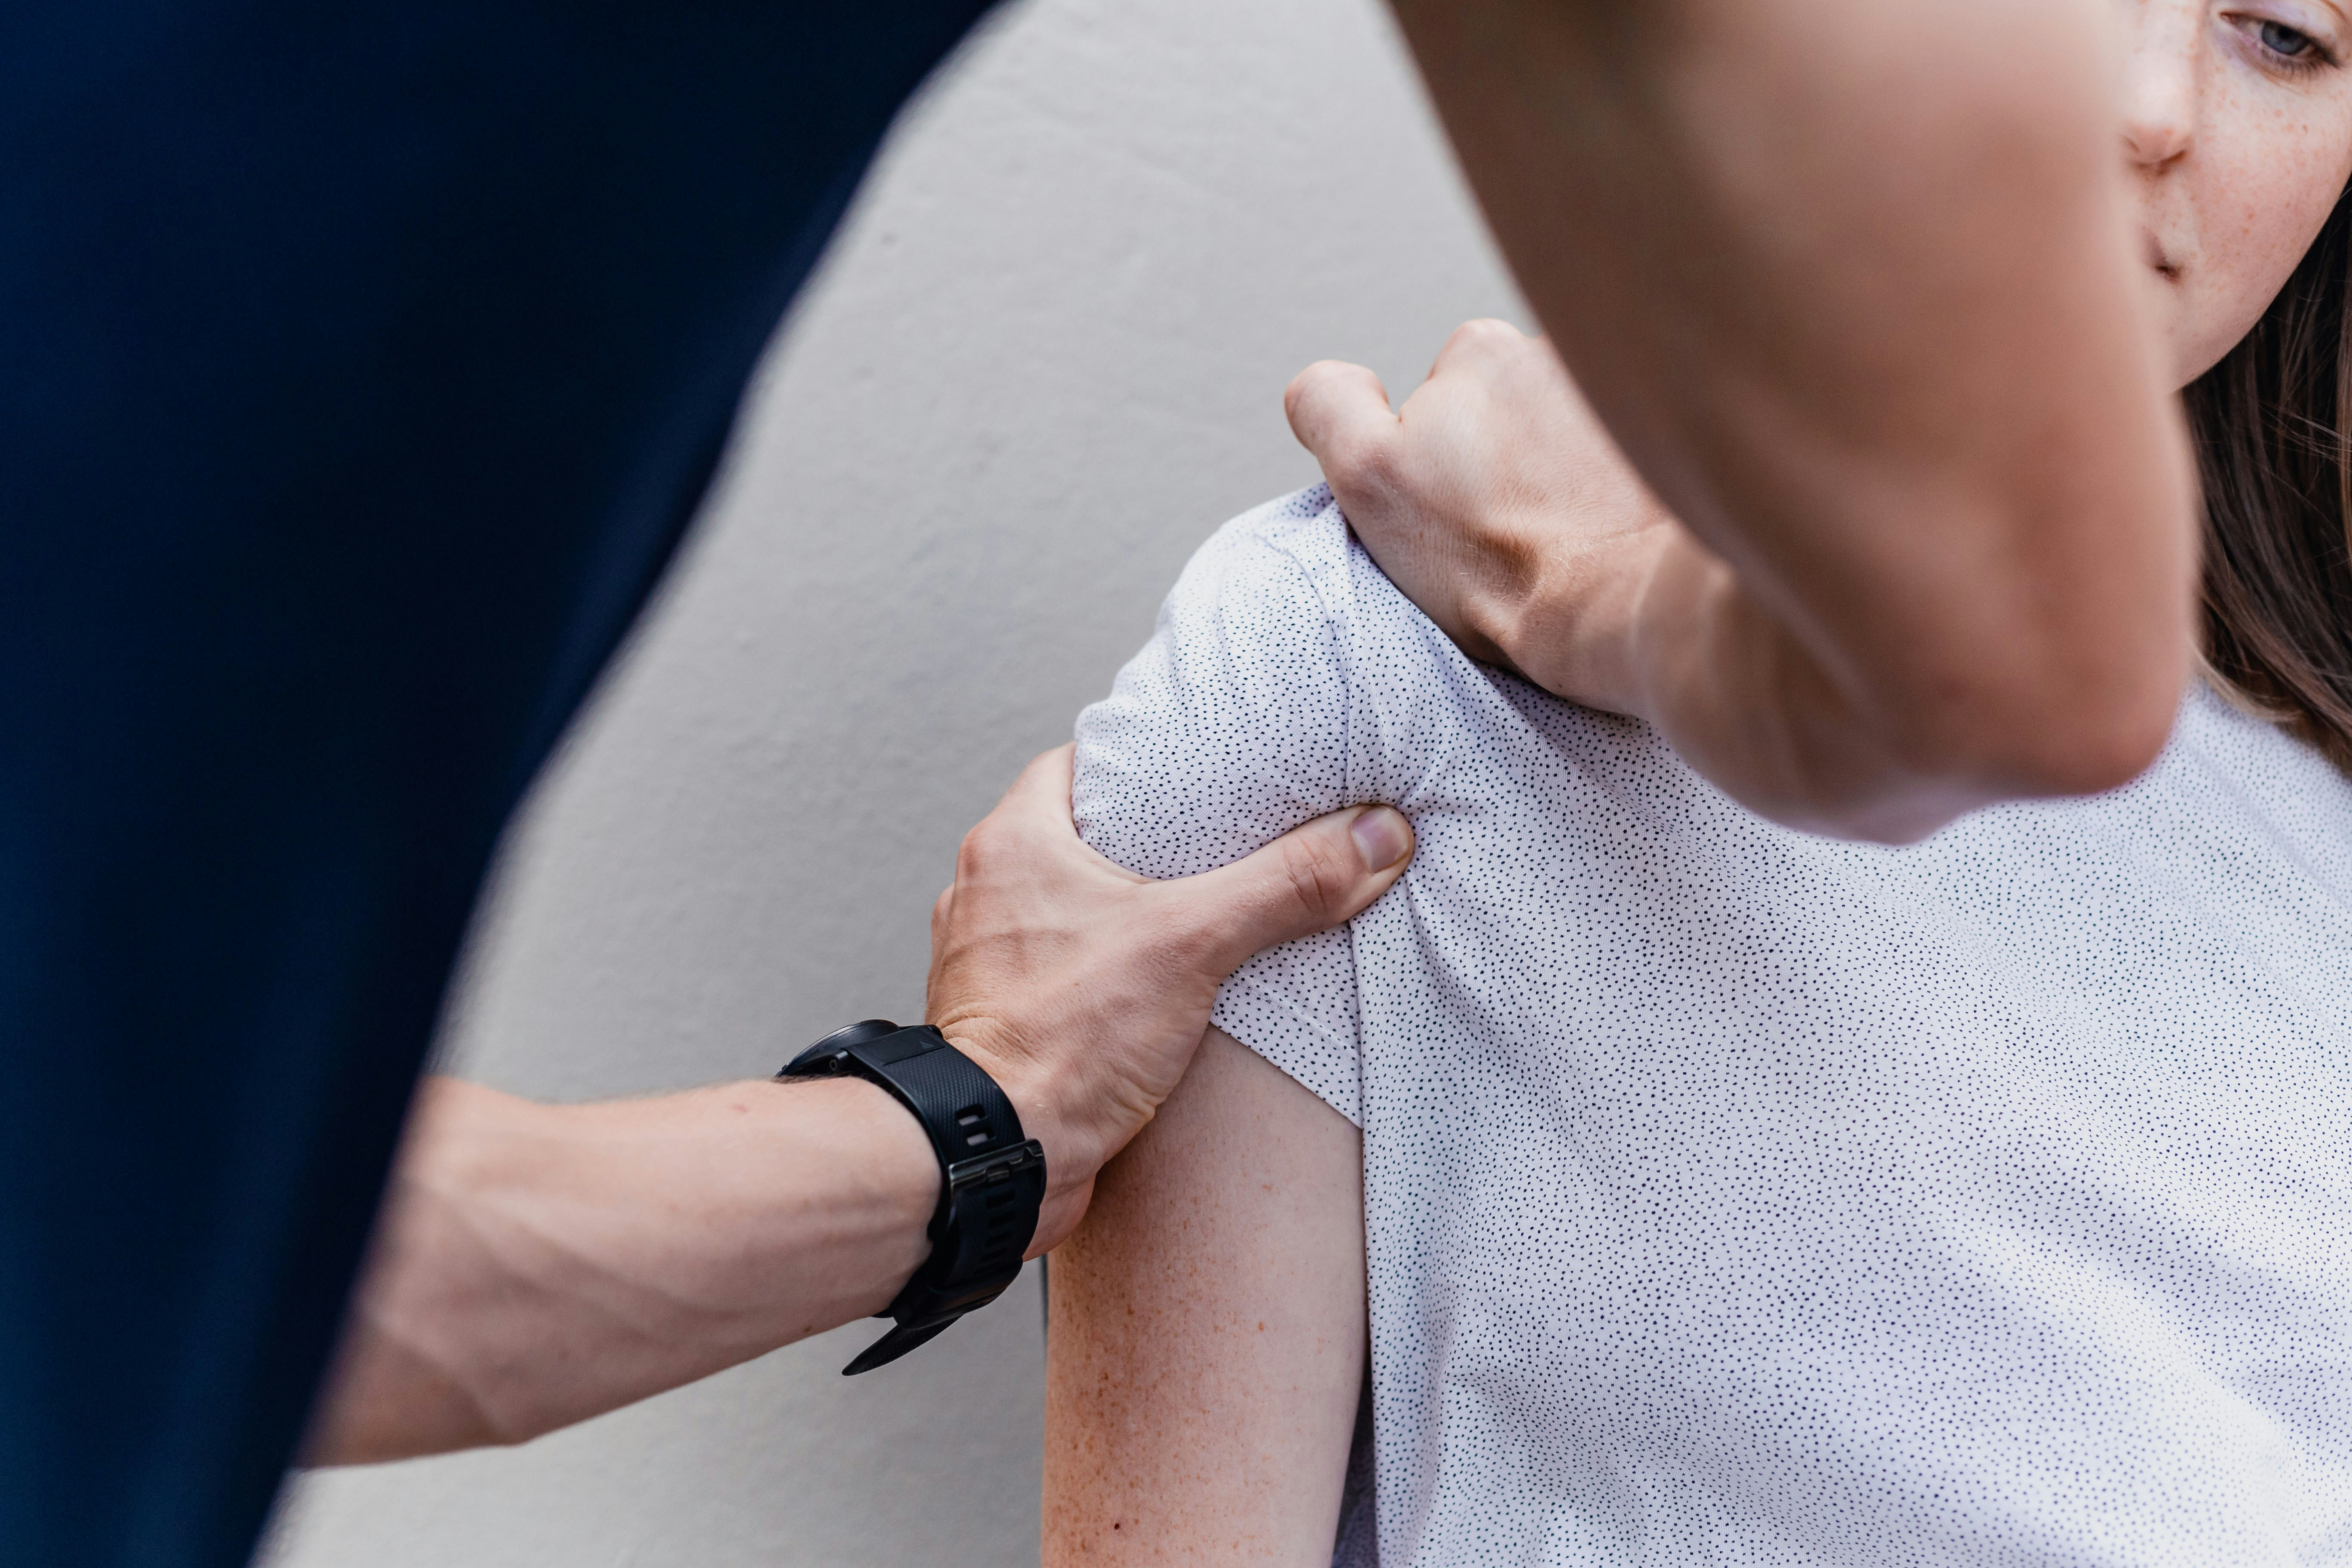
\includegraphics[keepaspectratio]{T02_Probabilidad_files/mediabag/photo-1645005512968-.jpg}}

}

\caption{Fisioterapeuta evaluando a un paciente}

\end{figure}%

\emph{Cada paciente es único. La probabilidad nos da el lenguaje para
cuantificar la incertidumbre clínica y tomar decisiones informadas.}

\begin{center}\rule{0.5\linewidth}{0.5pt}\end{center}

\section{De la Probabilidad a las Variables
Aleatorias}\label{de-la-probabilidad-a-las-variables-aleatorias-1}


\includegraphics[width=0.72917in,height=\textheight,keepaspectratio]{logo.png}

Hasta aquí hemos modelado \textbf{eventos} (A, B, intersecciones,
condicionales). Ahora damos el salto a modelar \textbf{variables}:
magnitudes clínicas que varían de paciente a paciente. Una variable
aleatoria asigna un número a cada resultado incierto.

{\def\LTcaptype{none} % do not increment counter
\begin{longtable}[]{@{}
  >{\raggedright\arraybackslash}p{(\linewidth - 2\tabcolsep) * \real{0.4909}}
  >{\raggedright\arraybackslash}p{(\linewidth - 2\tabcolsep) * \real{0.5091}}@{}}
\toprule\noalign{}
\begin{minipage}[b]{\linewidth}\raggedright
\textbf{En T01 (Descriptiva)}
\end{minipage} & \begin{minipage}[b]{\linewidth}\raggedright
\textbf{En T02 (Probabilidad)}
\end{minipage} \\
\midrule\noalign{}
\endhead
\bottomrule\noalign{}
\endlastfoot
\(\bar{x}\) --- media muestral & \(\mu = E(X)\) --- esperanza
poblacional \\
\(s^2\) --- varianza muestral & \(\sigma^2 = \Var(X)\) --- varianza
poblacional \\
\(s\) --- desviación típica muestral & \(\sigma = \SD(X)\) ---
desviación típica poblacional \\
\(\hat{p}\) --- proporción muestral & \(p = P(X \in A)\) ---
probabilidad poblacional \\
Describías \textbf{tu muestra} & Modelas \textbf{la población} \\
\end{longtable}
}

\subsection{Variable aleatoria ---
Definición}\label{variable-aleatoria-definicion}

\emph{Para modelar matemáticamente la incertidumbre clínica, necesitamos
asignar valores numéricos a los resultados inciertos: esto es una
variable aleatoria.}

\begin{tcolorbox}[enhanced jigsaw, arc=.35mm, bottomrule=.15mm, bottomtitle=1mm, breakable, colback=white, colbacktitle=quarto-callout-note-color!10!white, colframe=quarto-callout-note-color-frame, coltitle=black, left=2mm, leftrule=.75mm, opacityback=0, opacitybacktitle=0.6, rightrule=.15mm, title=\textcolor{quarto-callout-note-color}{\faInfo}\hspace{0.5em}{Note}, titlerule=0mm, toprule=.15mm, toptitle=1mm]

Una \textbf{variable aleatoria (VA)} es una función que asigna un valor
numérico a cada resultado de un experimento aleatorio.

\end{tcolorbox}

\textbf{Tipos de variables aleatorias:}

{\def\LTcaptype{none} % do not increment counter
\begin{longtable}[]{@{}
  >{\raggedright\arraybackslash}p{(\linewidth - 4\tabcolsep) * \real{0.1429}}
  >{\raggedright\arraybackslash}p{(\linewidth - 4\tabcolsep) * \real{0.2857}}
  >{\raggedright\arraybackslash}p{(\linewidth - 4\tabcolsep) * \real{0.5714}}@{}}
\toprule\noalign{}
\begin{minipage}[b]{\linewidth}\raggedright
Tipo
\end{minipage} & \begin{minipage}[b]{\linewidth}\raggedright
Descripción
\end{minipage} & \begin{minipage}[b]{\linewidth}\raggedright
Ejemplo en Fisioterapia
\end{minipage} \\
\midrule\noalign{}
\endhead
\bottomrule\noalign{}
\endlastfoot
\textbf{Discreta} & Toma valores aislados (contables) & Nº de sesiones
hasta mejoría \\
\textbf{Continua} & Toma cualquier valor en un intervalo & Rango de
movimiento (grados) \\
\end{longtable}
}

\textbf{Función de probabilidad / densidad:} Describe el comportamiento
probabilístico de la VA. Para discretas usamos la \textbf{función de
masa} \(P(X=x)\). Para continuas, la \textbf{función de densidad}
\(f(x)\) donde el área bajo la curva entre \(a\) y \(b\) es
\(P(a \leq X \leq b)\).

\subsection{Función de masa de probabilidad --- Va
discreta}\label{funcion-de-masa-de-probabilidad-va-discreta}

\begin{tcolorbox}[enhanced jigsaw, arc=.35mm, bottomrule=.15mm, bottomtitle=1mm, breakable, colback=white, colbacktitle=quarto-callout-note-color!10!white, colframe=quarto-callout-note-color-frame, coltitle=black, left=2mm, leftrule=.75mm, opacityback=0, opacitybacktitle=0.6, rightrule=.15mm, title=\textcolor{quarto-callout-note-color}{\faInfo}\hspace{0.5em}{Note}, titlerule=0mm, toprule=.15mm, toptitle=1mm]

\textbf{f.m.p.:} \(P(X = x) = f(x)\) asigna una probabilidad a cada
valor posible de una VA discreta.

\end{tcolorbox}

\textbf{Propiedades:} (1) \(P(X = x) \geq 0\) para todo \(x\); (2)
\(\sum_x P(X = x) = 1\)

\textbf{Ejemplo clínico:} \(X\) = nº de pacientes con mejoría en 3
tratados (\(p=0.5\))

{\def\LTcaptype{none} % do not increment counter
\begin{longtable}[]{@{}lllll@{}}
\toprule\noalign{}
\(x\) & 0 & 1 & 2 & 3 \\
\midrule\noalign{}
\endhead
\bottomrule\noalign{}
\endlastfoot
\(P(X=x)\) & 1/8 = 0.125 & 3/8 = 0.375 & 3/8 = 0.375 & 1/8 = 0.125 \\
\end{longtable}
}

\begin{Shaded}
\begin{Highlighting}[]
\NormalTok{x }\OtherTok{\textless{}{-}} \DecValTok{0}\SpecialCharTok{:}\DecValTok{3}\NormalTok{; px }\OtherTok{\textless{}{-}} \FunctionTok{dbinom}\NormalTok{(x, }\DecValTok{3}\NormalTok{, }\FloatTok{0.5}\NormalTok{)}
\NormalTok{bp }\OtherTok{\textless{}{-}} \FunctionTok{barplot}\NormalTok{(px, }\AttributeTok{names=}\NormalTok{x, }\AttributeTok{col=}\StringTok{"lightgreen"}\NormalTok{, }\AttributeTok{ylim=}\FunctionTok{c}\NormalTok{(}\DecValTok{0}\NormalTok{,}\FloatTok{0.45}\NormalTok{),}
        \AttributeTok{main=}\StringTok{"Función de Masa de Probabilidad — VA Discreta"}\NormalTok{,}
        \AttributeTok{xlab=}\StringTok{"x (nº pacientes con mejoría)"}\NormalTok{, }\AttributeTok{ylab=}\StringTok{"P(X = x)"}\NormalTok{)}
\FunctionTok{text}\NormalTok{(bp, px}\FloatTok{+0.02}\NormalTok{, }\FunctionTok{paste0}\NormalTok{(px}\SpecialCharTok{*}\DecValTok{8}\NormalTok{,}\StringTok{"/8 = "}\NormalTok{, px), }\AttributeTok{font=}\DecValTok{2}\NormalTok{, }\AttributeTok{cex=}\FloatTok{0.95}\NormalTok{)}
\FunctionTok{abline}\NormalTok{(}\AttributeTok{h=}\DecValTok{0}\NormalTok{, }\AttributeTok{col=}\StringTok{"grey"}\NormalTok{)}
\end{Highlighting}
\end{Shaded}

\pandocbounded{
\includegraphics[keepaspectratio]{T02_Probabilidad_files/figure-pdf/unnamed-chunk-13-1.pdf}}

\textbf{Verificación:} \(\sum P(X=x) = 0.125+0.375+0.375+0.125 = 1.00\)
✓

\subsection{Esperanza matemática --- Va
discreta}\label{esperanza-matematica-va-discreta}

\begin{tcolorbox}[enhanced jigsaw, arc=.35mm, bottomrule=.15mm, bottomtitle=1mm, breakable, colback=white, colbacktitle=quarto-callout-note-color!10!white, colframe=quarto-callout-note-color-frame, coltitle=black, left=2mm, leftrule=.75mm, opacityback=0, opacitybacktitle=0.6, rightrule=.15mm, title=\textcolor{quarto-callout-note-color}{\faInfo}\hspace{0.5em}{Note}, titlerule=0mm, toprule=.15mm, toptitle=1mm]

\[E(X) = \sum_i x_i \cdot P(X = x_i)\]

La esperanza es el \textbf{valor esperado} o \textbf{media poblacional}
de la VA.

\end{tcolorbox}

\textbf{Ejemplo (mejoría en 3 pacientes):}

{\def\LTcaptype{none} % do not increment counter
\begin{longtable}[]{@{}lll@{}}
\toprule\noalign{}
\(x_i\) & \(P(X=x_i)\) & \(x_i \cdot P(X=x_i)\) \\
\midrule\noalign{}
\endhead
\bottomrule\noalign{}
\endlastfoot
0 & 1/8 & \(0 \times 1/8 = 0\) \\
1 & 3/8 & \(1 \times 3/8 = 3/8\) \\
2 & 3/8 & \(2 \times 3/8 = 6/8\) \\
3 & 1/8 & \(3 \times 1/8 = 3/8\) \\
\end{longtable}
}

\[E(X) = 0 + \frac{3}{8} + \frac{6}{8} + \frac{3}{8} = \frac{12}{8} = 1.5\]

\textbf{Interpretación:} En promedio se espera que \textbf{1.5 de cada 3
pacientes} muestren mejoría.

\subsection{Varianza --- Va discreta}\label{varianza-va-discreta}

\begin{tcolorbox}[enhanced jigsaw, arc=.35mm, bottomrule=.15mm, bottomtitle=1mm, breakable, colback=white, colbacktitle=quarto-callout-note-color!10!white, colframe=quarto-callout-note-color-frame, coltitle=black, left=2mm, leftrule=.75mm, opacityback=0, opacitybacktitle=0.6, rightrule=.15mm, title=\textcolor{quarto-callout-note-color}{\faInfo}\hspace{0.5em}{Note}, titlerule=0mm, toprule=.15mm, toptitle=1mm]

\[\text{Var}(X) = E[(X - \mu)^2] = \sum_i (x_i - \mu)^2 \cdot P(X=x_i)\]

Fórmula alternativa: \(\text{Var}(X) = E(X^2) - [E(X)]^2\)

\end{tcolorbox}

\textbf{Ejemplo (mejoría, \(\mu = 1.5\)):}

{\def\LTcaptype{none} % do not increment counter
\begin{longtable}[]{@{}llll@{}}
\toprule\noalign{}
\(x_i\) & \(P(X=x_i)\) & \((x_i - 1.5)^2\) &
\((x_i-1.5)^2 \cdot P(X=x_i)\) \\
\midrule\noalign{}
\endhead
\bottomrule\noalign{}
\endlastfoot
0 & 1/8 & 2.25 & 2.25 × 1/8 = 0.281 \\
1 & 3/8 & 0.25 & 0.25 × 3/8 = 0.094 \\
2 & 3/8 & 0.25 & 0.25 × 3/8 = 0.094 \\
3 & 1/8 & 2.25 & 2.25 × 1/8 = 0.281 \\
\end{longtable}
}

\[\text{Var}(X) = 0.281+0.094+0.094+0.281 = 0.75\]

\begin{Shaded}
\begin{Highlighting}[]
\NormalTok{x }\OtherTok{\textless{}{-}} \DecValTok{0}\SpecialCharTok{:}\DecValTok{3}\NormalTok{; px }\OtherTok{\textless{}{-}} \FunctionTok{dbinom}\NormalTok{(x, }\DecValTok{3}\NormalTok{, }\FloatTok{0.5}\NormalTok{)}
\NormalTok{mu }\OtherTok{\textless{}{-}} \FunctionTok{sum}\NormalTok{(x}\SpecialCharTok{*}\NormalTok{px)}
\FunctionTok{cat}\NormalTok{(}\StringTok{"E(X) ="}\NormalTok{, mu, }\StringTok{"  Var(X) ="}\NormalTok{, }\FunctionTok{sum}\NormalTok{((x}\SpecialCharTok{{-}}\NormalTok{mu)}\SpecialCharTok{\^{}}\DecValTok{2}\SpecialCharTok{*}\NormalTok{px),}
    \StringTok{"}\SpecialCharTok{\textbackslash{}n}\StringTok{Verificación: n·p·(1{-}p) ="}\NormalTok{, }\DecValTok{3}\SpecialCharTok{*}\FloatTok{0.5}\SpecialCharTok{*}\FloatTok{0.5}\NormalTok{)}
\end{Highlighting}
\end{Shaded}

\begin{verbatim}
E(X) = 1.5   Var(X) = 0.75 
Verificación: n·p·(1-p) = 0.75
\end{verbatim}

\subsection{Función de distribución acumulativa
(f.d.a.)}\label{funcion-de-distribucion-acumulativa-f.d.a.}

\begin{tcolorbox}[enhanced jigsaw, arc=.35mm, bottomrule=.15mm, bottomtitle=1mm, breakable, colback=white, colbacktitle=quarto-callout-note-color!10!white, colframe=quarto-callout-note-color-frame, coltitle=black, left=2mm, leftrule=.75mm, opacityback=0, opacitybacktitle=0.6, rightrule=.15mm, title=\textcolor{quarto-callout-note-color}{\faInfo}\hspace{0.5em}{Note}, titlerule=0mm, toprule=.15mm, toptitle=1mm]

\[F(x) = P(X \leq x)\]

La f.d.a. acumula la probabilidad desde \(-\infty\) hasta \(x\). Es
\textbf{no decreciente}, \(\lim_{x\to-\infty}F(x)=0\),
\(\lim_{x\to\infty}F(x)=1\), y \(P(a < X \leq b) = F(b) - F(a)\).

\end{tcolorbox}

\subsection{f.d.a. de la Normal --- Cálculo de
Probabilidades}\label{f.d.a.-de-la-normal-calculo-de-probabilidades}

\begin{Shaded}
\begin{Highlighting}[]
\NormalTok{mu }\OtherTok{\textless{}{-}} \DecValTok{30}\NormalTok{; sigma }\OtherTok{\textless{}{-}} \DecValTok{8}
\FunctionTok{curve}\NormalTok{(}\FunctionTok{pnorm}\NormalTok{(x, mu, sigma), mu}\DecValTok{{-}24}\NormalTok{, mu}\SpecialCharTok{+}\DecValTok{24}\NormalTok{, }\AttributeTok{lwd=}\DecValTok{3}\NormalTok{, }\AttributeTok{col=}\StringTok{"steelblue"}\NormalTok{,}
      \AttributeTok{main=}\FunctionTok{expression}\NormalTok{(}\FunctionTok{paste}\NormalTok{(}\StringTok{"f.d.a. Normal: F(x) = P(X ≤ x),  N(30,"}\NormalTok{, }\DecValTok{8}\SpecialCharTok{\^{}}\DecValTok{2}\NormalTok{, }\StringTok{")"}\NormalTok{)),}
      \AttributeTok{xlab=}\StringTok{"Fuerza de prensión (kg)"}\NormalTok{, }\AttributeTok{ylab=}\StringTok{"F(x)"}\NormalTok{)}
\FunctionTok{abline}\NormalTok{(}\AttributeTok{h=}\FunctionTok{c}\NormalTok{(}\DecValTok{0}\NormalTok{,}\FloatTok{0.5}\NormalTok{,}\DecValTok{1}\NormalTok{), }\AttributeTok{lty=}\DecValTok{3}\NormalTok{, }\AttributeTok{col=}\StringTok{"grey"}\NormalTok{); }\FunctionTok{abline}\NormalTok{(}\AttributeTok{v=}\NormalTok{mu, }\AttributeTok{lty=}\DecValTok{2}\NormalTok{, }\AttributeTok{col=}\StringTok{"darkgreen"}\NormalTok{)}
\CommentTok{\# Marcar F(22)}
\FunctionTok{arrows}\NormalTok{(}\DecValTok{22}\NormalTok{, }\DecValTok{0}\NormalTok{, }\DecValTok{22}\NormalTok{, }\FunctionTok{pnorm}\NormalTok{(}\DecValTok{22}\NormalTok{, mu, sigma), }\AttributeTok{col=}\StringTok{"darkgreen"}\NormalTok{, }\AttributeTok{lwd=}\DecValTok{2}\NormalTok{, }\AttributeTok{length=}\FloatTok{0.1}\NormalTok{)}
\FunctionTok{points}\NormalTok{(}\DecValTok{22}\NormalTok{, }\FunctionTok{pnorm}\NormalTok{(}\DecValTok{22}\NormalTok{, mu, sigma), }\AttributeTok{pch=}\DecValTok{19}\NormalTok{, }\AttributeTok{col=}\StringTok{"darkgreen"}\NormalTok{, }\AttributeTok{cex=}\FloatTok{1.5}\NormalTok{)}
\FunctionTok{text}\NormalTok{(}\DecValTok{22}\NormalTok{, }\FunctionTok{pnorm}\NormalTok{(}\DecValTok{22}\NormalTok{,mu,sigma)}\SpecialCharTok{+}\FloatTok{0.05}\NormalTok{, }\FunctionTok{paste0}\NormalTok{(}\StringTok{"F(22) = "}\NormalTok{, }\FunctionTok{round}\NormalTok{(}\FunctionTok{pnorm}\NormalTok{(}\DecValTok{22}\NormalTok{,mu,sigma),}\DecValTok{3}\NormalTok{)), }\AttributeTok{col=}\StringTok{"darkgreen"}\NormalTok{, }\AttributeTok{font=}\DecValTok{2}\NormalTok{)}
\end{Highlighting}
\end{Shaded}

\pandocbounded{
\includegraphics[keepaspectratio]{T02_Probabilidad_files/figure-pdf/unnamed-chunk-15-1.pdf}}

\[F(22) = P(X \leq 22) = \Phi\left(\frac{22-30}{8}\right) = \Phi(-1) = 0.159\]

\subsection{f.d.a. --- VA Discreta vs VA
Continua}\label{f.d.a.-va-discreta-vs-va-continua}

\begin{Shaded}
\begin{Highlighting}[]
\FunctionTok{par}\NormalTok{(}\AttributeTok{mfrow=}\FunctionTok{c}\NormalTok{(}\DecValTok{1}\NormalTok{,}\DecValTok{2}\NormalTok{), }\AttributeTok{mar=}\FunctionTok{c}\NormalTok{(}\DecValTok{4}\NormalTok{,}\DecValTok{4}\NormalTok{,}\DecValTok{3}\NormalTok{,}\DecValTok{1}\NormalTok{))}

\CommentTok{\# DISCRETA: Binomial(10, 0.4) — funcion escalonada}
\NormalTok{x\_d }\OtherTok{\textless{}{-}} \DecValTok{0}\SpecialCharTok{:}\DecValTok{10}\NormalTok{; Fx\_d }\OtherTok{\textless{}{-}} \FunctionTok{pbinom}\NormalTok{(x\_d, }\DecValTok{10}\NormalTok{, }\FloatTok{0.4}\NormalTok{)}
\FunctionTok{plot}\NormalTok{(x\_d, Fx\_d, }\AttributeTok{type=}\StringTok{"s"}\NormalTok{, }\AttributeTok{lwd=}\DecValTok{3}\NormalTok{, }\AttributeTok{col=}\StringTok{"steelblue"}\NormalTok{,}
     \AttributeTok{main=}\StringTok{"f.d.a. Discreta — Binomial(10,0.4)"}\NormalTok{,}
     \AttributeTok{xlab=}\StringTok{"x"}\NormalTok{, }\AttributeTok{ylab=}\StringTok{"F(x)"}\NormalTok{, }\AttributeTok{ylim=}\FunctionTok{c}\NormalTok{(}\DecValTok{0}\NormalTok{,}\DecValTok{1}\NormalTok{), }\AttributeTok{xlim=}\FunctionTok{c}\NormalTok{(}\SpecialCharTok{{-}}\FloatTok{0.5}\NormalTok{,}\FloatTok{10.5}\NormalTok{))}
\FunctionTok{abline}\NormalTok{(}\AttributeTok{h=}\FunctionTok{c}\NormalTok{(}\DecValTok{0}\NormalTok{,}\FloatTok{0.5}\NormalTok{,}\DecValTok{1}\NormalTok{), }\AttributeTok{lty=}\DecValTok{3}\NormalTok{, }\AttributeTok{col=}\StringTok{"grey"}\NormalTok{); }\FunctionTok{points}\NormalTok{(x\_d, Fx\_d, }\AttributeTok{pch=}\DecValTok{19}\NormalTok{, }\AttributeTok{col=}\StringTok{"steelblue"}\NormalTok{, }\AttributeTok{cex=}\FloatTok{1.2}\NormalTok{)}

\CommentTok{\# CONTINUA: Normal(0,1) — función continua}
\FunctionTok{curve}\NormalTok{(}\FunctionTok{pnorm}\NormalTok{(x), }\SpecialCharTok{{-}}\DecValTok{4}\NormalTok{, }\DecValTok{4}\NormalTok{, }\AttributeTok{lwd=}\DecValTok{3}\NormalTok{, }\AttributeTok{col=}\StringTok{"seagreen"}\NormalTok{,}
      \AttributeTok{main=}\StringTok{"f.d.a. Continua — Normal(0,1)"}\NormalTok{,}
      \AttributeTok{xlab=}\StringTok{"x"}\NormalTok{, }\AttributeTok{ylab=}\StringTok{"F(x)"}\NormalTok{, }\AttributeTok{ylim=}\FunctionTok{c}\NormalTok{(}\DecValTok{0}\NormalTok{,}\DecValTok{1}\NormalTok{))}
\FunctionTok{abline}\NormalTok{(}\AttributeTok{h=}\FunctionTok{c}\NormalTok{(}\DecValTok{0}\NormalTok{,}\FloatTok{0.5}\NormalTok{,}\DecValTok{1}\NormalTok{), }\AttributeTok{lty=}\DecValTok{3}\NormalTok{, }\AttributeTok{col=}\StringTok{"grey"}\NormalTok{); }\FunctionTok{abline}\NormalTok{(}\AttributeTok{v=}\DecValTok{0}\NormalTok{, }\AttributeTok{lty=}\DecValTok{3}\NormalTok{, }\AttributeTok{col=}\StringTok{"grey"}\NormalTok{)}
\FunctionTok{points}\NormalTok{(}\DecValTok{0}\NormalTok{, }\FloatTok{0.5}\NormalTok{, }\AttributeTok{pch=}\DecValTok{19}\NormalTok{, }\AttributeTok{col=}\StringTok{"darkgreen"}\NormalTok{, }\AttributeTok{cex=}\FloatTok{1.5}\NormalTok{)}
\end{Highlighting}
\end{Shaded}

\pandocbounded{
\includegraphics[keepaspectratio]{T02_Probabilidad_files/figure-pdf/unnamed-chunk-16-1.pdf}}

\begin{Shaded}
\begin{Highlighting}[]
\FunctionTok{par}\NormalTok{(}\AttributeTok{mfrow=}\FunctionTok{c}\NormalTok{(}\DecValTok{1}\NormalTok{,}\DecValTok{1}\NormalTok{))}
\end{Highlighting}
\end{Shaded}

\textbf{VA Discreta:} \(F(x) = \sum_{x_i \leq x} P(X=x_i)\) →
\textbf{función escalonada}, salta en cada valor posible

\textbf{VA Continua:} \(F(x) = \int_{-\infty}^x f(t)dt\) →
\textbf{función continua suave}, sin saltos

\subsection{Función de densidad --- Va
continua}\label{funcion-de-densidad-va-continua}

\begin{tcolorbox}[enhanced jigsaw, arc=.35mm, bottomrule=.15mm, bottomtitle=1mm, breakable, colback=white, colbacktitle=quarto-callout-note-color!10!white, colframe=quarto-callout-note-color-frame, coltitle=black, left=2mm, leftrule=.75mm, opacityback=0, opacitybacktitle=0.6, rightrule=.15mm, title=\textcolor{quarto-callout-note-color}{\faInfo}\hspace{0.5em}{Note}, titlerule=0mm, toprule=.15mm, toptitle=1mm]

\[P(a \leq X \leq b) = \text{área bajo } f(x) \text{ entre } a \text{ y } b\]

La probabilidad es el \textbf{área bajo la curva} de la función de
densidad \(f(x)\).

\end{tcolorbox}

\textbf{Propiedades:} (1) \(f(x) \geq 0\); (2) área total bajo \(f(x)\)
= 1; (3) \(P(X=c) = 0\) para cualquier \(c\)

\begin{tcolorbox}[enhanced jigsaw, arc=.35mm, bottomrule=.15mm, bottomtitle=1mm, breakable, colback=white, colbacktitle=quarto-callout-tip-color!10!white, colframe=quarto-callout-tip-color-frame, coltitle=black, left=2mm, leftrule=.75mm, opacityback=0, opacitybacktitle=0.6, rightrule=.15mm, title=\textcolor{quarto-callout-tip-color}{\faLightbulb}\hspace{0.5em}{Tip}, titlerule=0mm, toprule=.15mm, toptitle=1mm]

\textbf{Notación:} El símbolo \(\int_a^b f(x)dx\) significa ``área bajo
la curva \(f(x)\) entre \(a\) y \(b\)''. En este curso \textbf{siempre
usaremos R} (\texttt{pnorm}, \texttt{dnorm}, \texttt{pt},
\texttt{pchisq}) en lugar de calcular integrales a mano.

\end{tcolorbox}

\begin{Shaded}
\begin{Highlighting}[]
\FunctionTok{set.seed}\NormalTok{(}\DecValTok{123}\NormalTok{)}
\NormalTok{ROM }\OtherTok{\textless{}{-}} \FunctionTok{rnorm}\NormalTok{(}\DecValTok{500}\NormalTok{, }\AttributeTok{mean=}\DecValTok{150}\NormalTok{, }\AttributeTok{sd=}\DecValTok{20}\NormalTok{)}
\FunctionTok{hist}\NormalTok{(ROM, }\AttributeTok{col=}\StringTok{"steelblue"}\NormalTok{, }\AttributeTok{border=}\StringTok{"white"}\NormalTok{, }\AttributeTok{breaks=}\DecValTok{25}\NormalTok{, }\AttributeTok{freq=}\ConstantTok{FALSE}\NormalTok{,}
     \AttributeTok{main=}\StringTok{"f.d.p. — ROM de Hombro (n=500)"}\NormalTok{,}
     \AttributeTok{xlab=}\StringTok{"Grados de flexión"}\NormalTok{, }\AttributeTok{ylab=}\StringTok{"Densidad de probabilidad f(x)"}\NormalTok{, }\AttributeTok{cex.lab=}\FloatTok{1.1}\NormalTok{)}
\FunctionTok{curve}\NormalTok{(}\FunctionTok{dnorm}\NormalTok{(x, }\DecValTok{150}\NormalTok{, }\DecValTok{20}\NormalTok{), }\AttributeTok{add=}\ConstantTok{TRUE}\NormalTok{, }\AttributeTok{col=}\StringTok{"darkgreen"}\NormalTok{, }\AttributeTok{lwd=}\DecValTok{3}\NormalTok{)}

\CommentTok{\# Sombrear P(130 ≤ X ≤ 170)}
\NormalTok{xr }\OtherTok{\textless{}{-}} \FunctionTok{seq}\NormalTok{(}\DecValTok{130}\NormalTok{, }\DecValTok{170}\NormalTok{, }\FloatTok{0.5}\NormalTok{); yr }\OtherTok{\textless{}{-}} \FunctionTok{dnorm}\NormalTok{(xr, }\DecValTok{150}\NormalTok{, }\DecValTok{20}\NormalTok{)}
\FunctionTok{polygon}\NormalTok{(}\FunctionTok{c}\NormalTok{(xr, }\FunctionTok{rev}\NormalTok{(xr)), }\FunctionTok{c}\NormalTok{(yr, }\FunctionTok{rep}\NormalTok{(}\DecValTok{0}\NormalTok{,}\FunctionTok{length}\NormalTok{(yr))), }\AttributeTok{col=}\FunctionTok{rgb}\NormalTok{(}\DecValTok{0}\NormalTok{,}\FloatTok{0.5}\NormalTok{,}\FloatTok{0.3}\NormalTok{,}\FloatTok{0.25}\NormalTok{), }\AttributeTok{border=}\ConstantTok{NA}\NormalTok{)}
\FunctionTok{text}\NormalTok{(}\DecValTok{150}\NormalTok{, }\FloatTok{0.003}\NormalTok{, }\FunctionTok{paste}\NormalTok{(}\StringTok{"P(130≤X≤170) ="}\NormalTok{,}
    \FunctionTok{round}\NormalTok{(}\FunctionTok{pnorm}\NormalTok{(}\DecValTok{170}\NormalTok{,}\DecValTok{150}\NormalTok{,}\DecValTok{20}\NormalTok{)}\SpecialCharTok{{-}}\FunctionTok{pnorm}\NormalTok{(}\DecValTok{130}\NormalTok{,}\DecValTok{150}\NormalTok{,}\DecValTok{20}\NormalTok{),}\DecValTok{3}\NormalTok{)), }\AttributeTok{font=}\DecValTok{2}\NormalTok{, }\AttributeTok{cex=}\FloatTok{1.1}\NormalTok{, }\AttributeTok{col=}\StringTok{"darkgreen"}\NormalTok{)}
\end{Highlighting}
\end{Shaded}

\pandocbounded{
\includegraphics[keepaspectratio]{T02_Probabilidad_files/figure-pdf/unnamed-chunk-17-1.pdf}}

\subsection{Esperanza y varianza --- Va
continua}\label{esperanza-y-varianza-va-continua}

\begin{tcolorbox}[enhanced jigsaw, arc=.35mm, bottomrule=.15mm, bottomtitle=1mm, breakable, colback=white, colbacktitle=quarto-callout-note-color!10!white, colframe=quarto-callout-note-color-frame, coltitle=black, left=2mm, leftrule=.75mm, opacityback=0, opacitybacktitle=0.6, rightrule=.15mm, title=\textcolor{quarto-callout-note-color}{\faInfo}\hspace{0.5em}{Note}, titlerule=0mm, toprule=.15mm, toptitle=1mm]

\[E(X) = \int_{-\infty}^{\infty} x \cdot f(x)\,dx \qquad \text{Var}(X) = \int_{-\infty}^{\infty} (x-\mu)^2 \cdot f(x)\,dx\]

\end{tcolorbox}

\textbf{Ejemplo --- ROM de hombro (\(\mu=150\), \(\sigma=20\)):}

\begin{Shaded}
\begin{Highlighting}[]
\FunctionTok{set.seed}\NormalTok{(}\DecValTok{123}\NormalTok{)}
\NormalTok{ROM }\OtherTok{\textless{}{-}} \FunctionTok{rnorm}\NormalTok{(}\DecValTok{10000}\NormalTok{, }\DecValTok{150}\NormalTok{, }\DecValTok{20}\NormalTok{)}
\FunctionTok{cat}\NormalTok{(}\StringTok{"E(X) teórica = 150°   E(X) simulada ="}\NormalTok{, }\FunctionTok{round}\NormalTok{(}\FunctionTok{mean}\NormalTok{(ROM),}\DecValTok{1}\NormalTok{), }\StringTok{"°"}\NormalTok{,}
    \StringTok{"}\SpecialCharTok{\textbackslash{}n}\StringTok{Var(X) teórica = 400   Var(X) simulada ="}\NormalTok{, }\FunctionTok{round}\NormalTok{(}\FunctionTok{var}\NormalTok{(ROM),}\DecValTok{1}\NormalTok{),}
    \StringTok{"}\SpecialCharTok{\textbackslash{}n}\StringTok{σ teórica = 20°   σ simulada ="}\NormalTok{, }\FunctionTok{round}\NormalTok{(}\FunctionTok{sd}\NormalTok{(ROM),}\DecValTok{1}\NormalTok{), }\StringTok{"°"}\NormalTok{)}
\end{Highlighting}
\end{Shaded}

\begin{verbatim}
E(X) teórica = 150°   E(X) simulada = 150 ° 
Var(X) teórica = 400   Var(X) simulada = 398.9 
σ teórica = 20°   σ simulada = 20 °
\end{verbatim}

\begin{Shaded}
\begin{Highlighting}[]
\CommentTok{\# Comparación de dos VA continuas con distinta dispersión}
\FunctionTok{curve}\NormalTok{(}\FunctionTok{dnorm}\NormalTok{(x, }\DecValTok{150}\NormalTok{, }\DecValTok{10}\NormalTok{), }\DecValTok{110}\NormalTok{, }\DecValTok{190}\NormalTok{, }\AttributeTok{col=}\StringTok{"steelblue"}\NormalTok{, }\AttributeTok{lwd=}\DecValTok{3}\NormalTok{,}
      \AttributeTok{main=}\FunctionTok{expression}\NormalTok{(}\FunctionTok{paste}\NormalTok{(}\StringTok{"Dos VA Normales: misma "}\NormalTok{, mu, }\StringTok{", distinta "}\NormalTok{, sigma)),}
      \AttributeTok{xlab=}\StringTok{"Grados ROM"}\NormalTok{, }\AttributeTok{ylab=}\StringTok{"f(x)"}\NormalTok{, }\AttributeTok{cex.lab=}\FloatTok{1.1}\NormalTok{)}
\FunctionTok{curve}\NormalTok{(}\FunctionTok{dnorm}\NormalTok{(x, }\DecValTok{150}\NormalTok{, }\DecValTok{25}\NormalTok{), }\DecValTok{110}\NormalTok{, }\DecValTok{190}\NormalTok{, }\AttributeTok{col=}\StringTok{"seagreen"}\NormalTok{, }\AttributeTok{lwd=}\DecValTok{3}\NormalTok{, }\AttributeTok{add=}\ConstantTok{TRUE}\NormalTok{)}
\FunctionTok{abline}\NormalTok{(}\AttributeTok{v=}\DecValTok{150}\NormalTok{, }\AttributeTok{lty=}\DecValTok{2}\NormalTok{, }\AttributeTok{col=}\StringTok{"grey"}\NormalTok{)}
\FunctionTok{legend}\NormalTok{(}\StringTok{"topright"}\NormalTok{, }\FunctionTok{c}\NormalTok{(}\FunctionTok{expression}\NormalTok{(sigma}\SpecialCharTok{==}\DecValTok{10}\NormalTok{), }\FunctionTok{expression}\NormalTok{(sigma}\SpecialCharTok{==}\DecValTok{25}\NormalTok{)),}
       \AttributeTok{col=}\FunctionTok{c}\NormalTok{(}\StringTok{"steelblue"}\NormalTok{,}\StringTok{"coral"}\NormalTok{), }\AttributeTok{lwd=}\DecValTok{3}\NormalTok{, }\AttributeTok{bty=}\StringTok{"n"}\NormalTok{, }\AttributeTok{cex=}\FloatTok{1.2}\NormalTok{)}
\FunctionTok{text}\NormalTok{(}\DecValTok{150}\NormalTok{, }\FloatTok{0.04}\NormalTok{, }\FunctionTok{expression}\NormalTok{(mu}\SpecialCharTok{==}\DecValTok{150}\NormalTok{), }\AttributeTok{pos=}\DecValTok{1}\NormalTok{, }\AttributeTok{cex=}\FloatTok{1.1}\NormalTok{)}
\end{Highlighting}
\end{Shaded}

\pandocbounded{
\includegraphics[keepaspectratio]{T02_Probabilidad_files/figure-pdf/unnamed-chunk-19-1.pdf}}

\textbf{Interpretación:} Ambas tienen la misma esperanza (\(\mu=150°\)),
pero la distribución naranja (\(\sigma=25\)) tiene \textbf{mayor
dispersión} que la azul (\(\sigma=10\)).

\subsection{Comparativa: Discreta vs continua --- Conceptos
análogos}\label{comparativa-discreta-vs-continua-conceptos-analogos}

{\def\LTcaptype{none} % do not increment counter
\begin{longtable}[]{@{}
  >{\raggedright\arraybackslash}p{(\linewidth - 4\tabcolsep) * \real{0.3125}}
  >{\raggedright\arraybackslash}p{(\linewidth - 4\tabcolsep) * \real{0.3438}}
  >{\raggedright\arraybackslash}p{(\linewidth - 4\tabcolsep) * \real{0.3438}}@{}}
\toprule\noalign{}
\begin{minipage}[b]{\linewidth}\raggedright
Concepto
\end{minipage} & \begin{minipage}[b]{\linewidth}\raggedright
VA Discreta
\end{minipage} & \begin{minipage}[b]{\linewidth}\raggedright
VA Continua
\end{minipage} \\
\midrule\noalign{}
\endhead
\bottomrule\noalign{}
\endlastfoot
\textbf{Función de probabilidad} & f.m.p.: \(P(X=x)\) & f.d.p.:
\(f(x)\) \\
\textbf{Probabilidad en intervalo} & \(\sum_{x \in [a,b]} P(X=x)\) &
\(\int_a^b f(x)\,dx\) \\
\textbf{Probabilidad puntual} & \(P(X=x) \geq 0\) & \(P(X=x) = 0\) \\
\textbf{f.d.a.} & \(F(x) = \sum_{x_i \leq x} P(X=x_i)\) &
\(F(x) = \int_{-\infty}^x f(t)\,dt\) \\
\textbf{Normalización} & \(\sum_x P(X=x) = 1\) &
\(\int_{-\infty}^{\infty} f(x)\,dx = 1\) \\
\textbf{Esperanza \(E(X)\)} & \(\sum x_i \cdot P(X=x_i)\) &
\(\int x \cdot f(x)\,dx\) \\
\textbf{Varianza \(\text{Var}(X)\)} &
\(\sum (x_i-\mu)^2 \cdot P(X=x_i)\) &
\(\int (x-\mu)^2 \cdot f(x)\,dx\) \\
\end{longtable}
}

\begin{Shaded}
\begin{Highlighting}[]
\FunctionTok{par}\NormalTok{(}\AttributeTok{mfrow=}\FunctionTok{c}\NormalTok{(}\DecValTok{1}\NormalTok{,}\DecValTok{2}\NormalTok{), }\AttributeTok{mar=}\FunctionTok{c}\NormalTok{(}\DecValTok{4}\NormalTok{,}\DecValTok{4}\NormalTok{,}\DecValTok{3}\NormalTok{,}\DecValTok{1}\NormalTok{))}
\CommentTok{\# Discreta: Binomial}
\NormalTok{x }\OtherTok{\textless{}{-}} \DecValTok{0}\SpecialCharTok{:}\DecValTok{10}
\FunctionTok{plot}\NormalTok{(x, }\FunctionTok{dbinom}\NormalTok{(x,}\DecValTok{10}\NormalTok{,}\FloatTok{0.5}\NormalTok{), }\AttributeTok{type=}\StringTok{"h"}\NormalTok{, }\AttributeTok{lwd=}\DecValTok{4}\NormalTok{, }\AttributeTok{col=}\StringTok{"steelblue"}\NormalTok{,}
     \AttributeTok{main=}\StringTok{"VA Discreta: Binomial(10,0.5)"}\NormalTok{, }\AttributeTok{xlab=}\StringTok{"x"}\NormalTok{, }\AttributeTok{ylab=}\StringTok{"P(X=x)"}\NormalTok{)}
\CommentTok{\# Continua: Normal}
\FunctionTok{curve}\NormalTok{(}\FunctionTok{dnorm}\NormalTok{(x), }\SpecialCharTok{{-}}\DecValTok{4}\NormalTok{, }\DecValTok{4}\NormalTok{, }\AttributeTok{lwd=}\DecValTok{3}\NormalTok{, }\AttributeTok{col=}\StringTok{"seagreen"}\NormalTok{,}
      \AttributeTok{main=}\StringTok{"VA Continua: Normal(0,1)"}\NormalTok{, }\AttributeTok{xlab=}\StringTok{"x"}\NormalTok{, }\AttributeTok{ylab=}\StringTok{"f(x)"}\NormalTok{)}
\end{Highlighting}
\end{Shaded}

\pandocbounded{
\includegraphics[keepaspectratio]{T02_Probabilidad_files/figure-pdf/unnamed-chunk-20-1.pdf}}

\begin{Shaded}
\begin{Highlighting}[]
\FunctionTok{par}\NormalTok{(}\AttributeTok{mfrow=}\FunctionTok{c}\NormalTok{(}\DecValTok{1}\NormalTok{,}\DecValTok{1}\NormalTok{))}
\end{Highlighting}
\end{Shaded}

\subsection{Las cuatro funciones de R para
distribuciones}\label{las-cuatro-funciones-de-r-para-distribuciones}

{\def\LTcaptype{none} % do not increment counter
\begin{longtable}[]{@{}
  >{\raggedright\arraybackslash}p{(\linewidth - 6\tabcolsep) * \real{0.2045}}
  >{\raggedright\arraybackslash}p{(\linewidth - 6\tabcolsep) * \real{0.2045}}
  >{\raggedright\arraybackslash}p{(\linewidth - 6\tabcolsep) * \real{0.2045}}
  >{\raggedright\arraybackslash}p{(\linewidth - 6\tabcolsep) * \real{0.3864}}@{}}
\toprule\noalign{}
\begin{minipage}[b]{\linewidth}\raggedright
Prefijo
\end{minipage} & \begin{minipage}[b]{\linewidth}\raggedright
Función
\end{minipage} & \begin{minipage}[b]{\linewidth}\raggedright
Fórmula
\end{minipage} & \begin{minipage}[b]{\linewidth}\raggedright
Ejemplo (Normal)
\end{minipage} \\
\midrule\noalign{}
\endhead
\bottomrule\noalign{}
\endlastfoot
\texttt{d} & Densidad/Masa & \(f(x)\) & \texttt{dnorm(x,\ mean,\ sd)} \\
\texttt{p} & Distribución acumulada & \(F(x) = P(X \leq x)\) &
\texttt{pnorm(q,\ mean,\ sd)} \\
\texttt{q} & Cuantil (percentil) & \(F^{-1}(p)\) &
\texttt{qnorm(p,\ mean,\ sd)} \\
\texttt{r} & Aleatorio & Genera \(n\) valores &
\texttt{rnorm(n,\ mean,\ sd)} \\
\end{longtable}
}

\begin{tcolorbox}[enhanced jigsaw, arc=.35mm, bottomrule=.15mm, bottomtitle=1mm, breakable, colback=white, colbacktitle=quarto-callout-tip-color!10!white, colframe=quarto-callout-tip-color-frame, coltitle=black, left=2mm, leftrule=.75mm, opacityback=0, opacitybacktitle=0.6, rightrule=.15mm, title=\textcolor{quarto-callout-tip-color}{\faLightbulb}\hspace{0.5em}{Tip}, titlerule=0mm, toprule=.15mm, toptitle=1mm]

Este patrón se repite para todas las distribuciones: \texttt{dbinom},
\texttt{pbinom}, \texttt{qbinom}, \texttt{rbinom}; \texttt{dpois},
\texttt{ppois}, \texttt{qpois}, \texttt{rpois}, etc.

\end{tcolorbox}

\begin{center}\rule{0.5\linewidth}{0.5pt}\end{center}

\section{Herramientas Computacionales para
Distribuciones}\label{herramientas-computacionales-para-distribuciones}

\textbf{Conexión:} R dispone de funciones específicas para cada
distribución de probabilidad. Aprender a usarlas correctamente es tan
importante como entender la teoría.

\subsection{\texorpdfstring{\texttt{lower.tail} --- La Opción Más Útil
de las Funciones
\texttt{p}}{lower.tail --- La Opción Más Útil de las Funciones p}}\label{lower.tail-la-opcion-mas-util-de-las-funciones-p}

Todas las funciones \texttt{p} (acumuladas) tienen el argumento
\texttt{lower.tail}:

\textbf{\texttt{lower.tail\ =\ TRUE} (por defecto):}\\
- \texttt{pnorm(k)} = \(P(X \leq k)\)\\
- \texttt{pbinom(k,\ n,\ p)} = \(P(X \leq k)\)\\
- \texttt{ppois(k,\ lambda)} = \(P(X \leq k)\)

Calcula el área \textbf{desde \(-\infty\) hasta \(k\)}

\textbf{\texttt{lower.tail\ =\ FALSE}:}\\
- \texttt{pnorm(k,\ lower.tail=FALSE)} = \(P(X > k)\)\\
- \texttt{pbinom(k,\ n,\ p,\ lower.tail=FALSE)} = \(P(X > k)\)\\
- \texttt{ppois(k,\ lambda,\ lower.tail=FALSE)} = \(P(X > k)\)

Calcula el área \textbf{desde \(k\) hasta \(+\infty\)}

\textbf{Equivalencia fundamental:}

\begin{Shaded}
\begin{Highlighting}[]
\NormalTok{n}\OtherTok{\textless{}{-}}\DecValTok{10}\NormalTok{; p}\OtherTok{\textless{}{-}}\FloatTok{0.5}\NormalTok{; k}\OtherTok{\textless{}{-}}\DecValTok{3}
\CommentTok{\# Estas dos expresiones son EXACTAMENTE IGUALES:}
\FunctionTok{pbinom}\NormalTok{(k, n, p, }\AttributeTok{lower.tail=}\ConstantTok{FALSE}\NormalTok{)  }\CommentTok{\# P(X \textgreater{} 3)}
\end{Highlighting}
\end{Shaded}

\begin{verbatim}
[1] 0.828125
\end{verbatim}

\begin{Shaded}
\begin{Highlighting}[]
\DecValTok{1} \SpecialCharTok{{-}} \FunctionTok{pbinom}\NormalTok{(k, n, p)                }\CommentTok{\# 1 {-} P(X ≤ 3)}
\end{Highlighting}
\end{Shaded}

\begin{verbatim}
[1] 0.828125
\end{verbatim}

\begin{center}\rule{0.5\linewidth}{0.5pt}\end{center}

\subsection{\texorpdfstring{\texttt{lower.tail} --- Equivalencias y
Precauciones}{lower.tail --- Equivalencias y Precauciones}}\label{lower.tail-equivalencias-y-precauciones}

\textbf{Variables continuas (Normal, t, χ², F):}

\begin{Shaded}
\begin{Highlighting}[]
\CommentTok{\# P(X \textgreater{} 1.96) es IDÉNTICO a:}
\FunctionTok{pnorm}\NormalTok{(}\FloatTok{1.96}\NormalTok{, }\AttributeTok{lower.tail=}\ConstantTok{FALSE}\NormalTok{)}
\end{Highlighting}
\end{Shaded}

\begin{verbatim}
[1] 0.0249979
\end{verbatim}

\begin{Shaded}
\begin{Highlighting}[]
\DecValTok{1} \SpecialCharTok{{-}} \FunctionTok{pnorm}\NormalTok{(}\FloatTok{1.96}\NormalTok{)}
\end{Highlighting}
\end{Shaded}

\begin{verbatim}
[1] 0.0249979
\end{verbatim}

\textbf{Variables discretas (Binomial, Poisson):}

\begin{Shaded}
\begin{Highlighting}[]
\CommentTok{\# ¡CUIDADO! P(X \textgreater{} 3) ≠ P(X ≥ 3)}
\FunctionTok{pbinom}\NormalTok{(}\DecValTok{3}\NormalTok{, }\DecValTok{10}\NormalTok{, }\FloatTok{0.5}\NormalTok{, }\AttributeTok{lower.tail=}\ConstantTok{FALSE}\NormalTok{)  }\CommentTok{\# P(X \textgreater{} 3) = P(X ≥ 4)}
\end{Highlighting}
\end{Shaded}

\begin{verbatim}
[1] 0.828125
\end{verbatim}

\begin{Shaded}
\begin{Highlighting}[]
\DecValTok{1} \SpecialCharTok{{-}} \FunctionTok{pbinom}\NormalTok{(}\DecValTok{4{-}1}\NormalTok{, }\DecValTok{10}\NormalTok{, }\FloatTok{0.5}\NormalTok{)              }\CommentTok{\# P(X ≥ 4) = 1 {-} P(X ≤ 3)}
\end{Highlighting}
\end{Shaded}

\begin{verbatim}
[1] 0.828125
\end{verbatim}

{\def\LTcaptype{none} % do not increment counter
\begin{longtable}[]{@{}
  >{\raggedright\arraybackslash}p{(\linewidth - 4\tabcolsep) * \real{0.2969}}
  >{\raggedright\arraybackslash}p{(\linewidth - 4\tabcolsep) * \real{0.2812}}
  >{\raggedright\arraybackslash}p{(\linewidth - 4\tabcolsep) * \real{0.4219}}@{}}
\toprule\noalign{}
\begin{minipage}[b]{\linewidth}\raggedright
Quiero calcular\ldots{}
\end{minipage} & \begin{minipage}[b]{\linewidth}\raggedright
Normal (continua)
\end{minipage} & \begin{minipage}[b]{\linewidth}\raggedright
Binomial/Poisson (discreta)
\end{minipage} \\
\midrule\noalign{}
\endhead
\bottomrule\noalign{}
\endlastfoot
\(P(X \leq k)\) & \texttt{pnorm(k)} & \texttt{pbinom(k,\ n,\ p)} /
\texttt{ppois(k,\ λ)} \\
\(P(X < k)\) & \texttt{pnorm(k)} (= \(P(X \leq k)\)) &
\texttt{pbinom(k-1,\ n,\ p)} ⚠️ \\
\(P(X > k)\) & \texttt{pnorm(k,\ lower.tail=FALSE)} &
\texttt{pbinom(k,\ n,\ p,\ lower.tail=FALSE)} \\
\(P(X \geq k)\) & \texttt{pnorm(k,\ lower.tail=FALSE)} (= \(P(X > k)\))
& \texttt{1\ -\ pbinom(k-1,\ n,\ p)} ⚠️ \\
\end{longtable}
}

\begin{tcolorbox}[enhanced jigsaw, arc=.35mm, bottomrule=.15mm, bottomtitle=1mm, breakable, colback=white, colbacktitle=quarto-callout-warning-color!10!white, colframe=quarto-callout-warning-color-frame, coltitle=black, left=2mm, leftrule=.75mm, opacityback=0, opacitybacktitle=0.6, rightrule=.15mm, title=\textcolor{quarto-callout-warning-color}{\faExclamationTriangle}\hspace{0.5em}{Warning}, titlerule=0mm, toprule=.15mm, toptitle=1mm]

\textbf{Truco para estudiantes:} En variables \textbf{discretas}
(Binomial, Poisson), \(P(X < k) \neq P(X \leq k)\). La diferencia es
\(P(X=k)\). Usad \texttt{lower.tail=FALSE} para colas derechas y
recordad restar 1 al límite para desigualdades estrictas.

\end{tcolorbox}

\begin{center}\rule{0.5\linewidth}{0.5pt}\end{center}

\section{La Distribución Normal y sus
Aproximaciones}\label{la-distribucion-normal-y-sus-aproximaciones}

\textbf{Puente con T03 --- Estimación:} La distribución Normal es la
base del Teorema Central del Límite, que veremos en el Tema 3. Todo lo
que aprendas aquí sobre \texttt{pnorm()}, \texttt{qnorm()} y Z-scores se
usará para construir intervalos de confianza y contrastes de hipótesis.

\subsection{Distribución Normal --- Historia y
contexto}\label{distribucion-normal-historia-y-contexto}

\textbf{Carl Friedrich Gauss (1777--1855)} introdujo esta distribución
estudiando errores de medición astronómica. Originalmente llamada
\textbf{``campana de Gauss''}, hoy es la distribución más importante en
estadística.

\textbf{¿Por qué es tan ubicua?} Por el \textbf{Teorema Central del
Límite}: la suma de muchas variables independientes tiende a una Normal,
sin importar su distribución original. Por eso aparece en biología,
medicina, economía, física\ldots{}

\begin{Shaded}
\begin{Highlighting}[]
\FunctionTok{curve}\NormalTok{(}\FunctionTok{dnorm}\NormalTok{(x, }\DecValTok{0}\NormalTok{, }\DecValTok{1}\NormalTok{), }\SpecialCharTok{{-}}\DecValTok{4}\NormalTok{, }\DecValTok{4}\NormalTok{, }\AttributeTok{lwd=}\DecValTok{3}\NormalTok{, }\AttributeTok{col=}\StringTok{"steelblue"}\NormalTok{,}
      \AttributeTok{main=}\FunctionTok{expression}\NormalTok{(}\FunctionTok{paste}\NormalTok{(}\StringTok{"Distribución Normal "}\NormalTok{, }\FunctionTok{N}\NormalTok{(mu, sigma}\SpecialCharTok{\^{}}\DecValTok{2}\NormalTok{))),}
      \AttributeTok{xlab=}\StringTok{"x"}\NormalTok{, }\AttributeTok{ylab=}\FunctionTok{expression}\NormalTok{(}\FunctionTok{f}\NormalTok{(x)))}
\CommentTok{\# μ ± σ (68\%)}
\NormalTok{x1}\OtherTok{\textless{}{-}}\FunctionTok{seq}\NormalTok{(}\SpecialCharTok{{-}}\DecValTok{1}\NormalTok{,}\DecValTok{1}\NormalTok{,}\FloatTok{0.01}\NormalTok{); }\FunctionTok{polygon}\NormalTok{(}\FunctionTok{c}\NormalTok{(x1,}\FunctionTok{rev}\NormalTok{(x1)),}\FunctionTok{c}\NormalTok{(}\FunctionTok{dnorm}\NormalTok{(x1),}\FunctionTok{rep}\NormalTok{(}\DecValTok{0}\NormalTok{,}\FunctionTok{length}\NormalTok{(x1))),}\AttributeTok{col=}\FunctionTok{rgb}\NormalTok{(}\DecValTok{0}\NormalTok{,}\DecValTok{0}\NormalTok{,}\DecValTok{1}\NormalTok{,}\FloatTok{0.2}\NormalTok{),}\AttributeTok{border=}\ConstantTok{NA}\NormalTok{)}
\CommentTok{\# μ ± 2σ (95\%)}
\NormalTok{x2}\OtherTok{\textless{}{-}}\FunctionTok{seq}\NormalTok{(}\SpecialCharTok{{-}}\DecValTok{2}\NormalTok{,}\DecValTok{2}\NormalTok{,}\FloatTok{0.01}\NormalTok{); }\FunctionTok{polygon}\NormalTok{(}\FunctionTok{c}\NormalTok{(x2,}\FunctionTok{rev}\NormalTok{(x2)),}\FunctionTok{c}\NormalTok{(}\FunctionTok{dnorm}\NormalTok{(x2),}\FunctionTok{rep}\NormalTok{(}\DecValTok{0}\NormalTok{,}\FunctionTok{length}\NormalTok{(x2))),}\AttributeTok{col=}\FunctionTok{rgb}\NormalTok{(}\DecValTok{0}\NormalTok{,}\DecValTok{0}\NormalTok{,}\DecValTok{1}\NormalTok{,}\FloatTok{0.1}\NormalTok{),}\AttributeTok{border=}\ConstantTok{NA}\NormalTok{)}
\FunctionTok{abline}\NormalTok{(}\AttributeTok{v=}\FunctionTok{c}\NormalTok{(}\SpecialCharTok{{-}}\DecValTok{2}\NormalTok{,}\SpecialCharTok{{-}}\DecValTok{1}\NormalTok{,}\DecValTok{0}\NormalTok{,}\DecValTok{1}\NormalTok{,}\DecValTok{2}\NormalTok{), }\AttributeTok{lty=}\FunctionTok{c}\NormalTok{(}\DecValTok{3}\NormalTok{,}\DecValTok{2}\NormalTok{,}\DecValTok{1}\NormalTok{,}\DecValTok{2}\NormalTok{,}\DecValTok{3}\NormalTok{), }\AttributeTok{col=}\FunctionTok{c}\NormalTok{(}\StringTok{"grey"}\NormalTok{,}\StringTok{"grey"}\NormalTok{,}\StringTok{"red"}\NormalTok{,}\StringTok{"grey"}\NormalTok{,}\StringTok{"grey"}\NormalTok{))}
\FunctionTok{text}\NormalTok{(}\DecValTok{0}\NormalTok{, }\FloatTok{0.25}\NormalTok{, }\StringTok{"68\%"}\NormalTok{, }\AttributeTok{cex=}\FloatTok{1.2}\NormalTok{); }\FunctionTok{text}\NormalTok{(}\DecValTok{0}\NormalTok{, }\FloatTok{0.05}\NormalTok{, }\StringTok{"95\%"}\NormalTok{, }\AttributeTok{cex=}\FloatTok{1.2}\NormalTok{)}
\end{Highlighting}
\end{Shaded}

\pandocbounded{
\includegraphics[keepaspectratio]{T02_Probabilidad_files/figure-pdf/unnamed-chunk-24-1.pdf}}

\textbf{La curva normal describe la distribución de errores y de
fenómenos naturales donde muchas causas pequeñas se suman.} Hoy, en
fisioterapia, modela: fuerza muscular, ROM articular, presión arterial,
y prácticamente cualquier variable biológica continua.

\subsection{Distribución Normal --- Fórmula y
propiedades}\label{distribucion-normal-formula-y-propiedades}

\begin{tcolorbox}[enhanced jigsaw, arc=.35mm, bottomrule=.15mm, bottomtitle=1mm, breakable, colback=white, colbacktitle=quarto-callout-note-color!10!white, colframe=quarto-callout-note-color-frame, coltitle=black, left=2mm, leftrule=.75mm, opacityback=0, opacitybacktitle=0.6, rightrule=.15mm, title=\textcolor{quarto-callout-note-color}{\faInfo}\hspace{0.5em}{Note}, titlerule=0mm, toprule=.15mm, toptitle=1mm]

\[f(x) = \frac{1}{\sigma\sqrt{2\pi}} \exp\left\{-\frac{(x-\mu)^2}{2\sigma^2}\right\}, \quad -\infty < x < \infty\]

\begin{itemize}
\tightlist
\item
  \(\mu\) = media (centro de la campana), \(\sigma\) = desviación típica
  (dispersión)
\item
  \(E(X) = \mu\), \(\text{Var}(X) = \sigma^2\)
\item
  \textbf{Simetrica:} media = mediana = moda
\item
  \(\mu \pm \sigma\) contiene ≈ 68\%, \(\mu \pm 2\sigma\) contiene ≈
  95\%, \(\mu \pm 3\sigma\) contiene ≈ 99.7\%
\end{itemize}

\end{tcolorbox}

\textbf{Ejemplo clínico:} Fuerza de prensión manual:
\(X \sim N(30, 8^2)\) kg

\subsection{Visualización de la distribución
Normal}\label{visualizacion-de-la-distribucion-normal}

\textbf{Efecto de cambiar \(\mu\) y \(\sigma\) en la forma de la
campana:}

\begin{Shaded}
\begin{Highlighting}[]
\FunctionTok{par}\NormalTok{(}\AttributeTok{mfrow=}\FunctionTok{c}\NormalTok{(}\DecValTok{1}\NormalTok{,}\DecValTok{2}\NormalTok{), }\AttributeTok{mar=}\FunctionTok{c}\NormalTok{(}\DecValTok{4}\NormalTok{,}\DecValTok{4}\NormalTok{,}\DecValTok{3}\NormalTok{,}\DecValTok{1}\NormalTok{))}
\CommentTok{\# Cambiar μ}
\FunctionTok{curve}\NormalTok{(}\FunctionTok{dnorm}\NormalTok{(x, }\DecValTok{0}\NormalTok{, }\DecValTok{1}\NormalTok{), }\SpecialCharTok{{-}}\DecValTok{5}\NormalTok{, }\DecValTok{8}\NormalTok{, }\AttributeTok{lwd=}\DecValTok{3}\NormalTok{, }\AttributeTok{col=}\StringTok{"steelblue"}\NormalTok{, }\AttributeTok{ylab=}\StringTok{"Densidad"}\NormalTok{,}
      \AttributeTok{main=}\FunctionTok{expression}\NormalTok{(}\FunctionTok{paste}\NormalTok{(}\StringTok{"Cambiando "}\NormalTok{, mu, }\StringTok{" ("}\NormalTok{, sigma, }\StringTok{"=1)"}\NormalTok{)), }\AttributeTok{xlab=}\StringTok{"x"}\NormalTok{)}
\FunctionTok{curve}\NormalTok{(}\FunctionTok{dnorm}\NormalTok{(x, }\DecValTok{2}\NormalTok{, }\DecValTok{1}\NormalTok{), }\SpecialCharTok{{-}}\DecValTok{5}\NormalTok{, }\DecValTok{8}\NormalTok{, }\AttributeTok{lwd=}\DecValTok{3}\NormalTok{, }\AttributeTok{col=}\StringTok{"seagreen"}\NormalTok{, }\AttributeTok{add=}\ConstantTok{TRUE}\NormalTok{)}
\FunctionTok{curve}\NormalTok{(}\FunctionTok{dnorm}\NormalTok{(x, }\DecValTok{4}\NormalTok{, }\DecValTok{1}\NormalTok{), }\SpecialCharTok{{-}}\DecValTok{5}\NormalTok{, }\DecValTok{8}\NormalTok{, }\AttributeTok{lwd=}\DecValTok{3}\NormalTok{, }\AttributeTok{col=}\StringTok{"darkgreen"}\NormalTok{, }\AttributeTok{add=}\ConstantTok{TRUE}\NormalTok{)}
\FunctionTok{abline}\NormalTok{(}\AttributeTok{v=}\FunctionTok{c}\NormalTok{(}\DecValTok{0}\NormalTok{,}\DecValTok{2}\NormalTok{,}\DecValTok{4}\NormalTok{), }\AttributeTok{lty=}\DecValTok{2}\NormalTok{, }\AttributeTok{col=}\FunctionTok{c}\NormalTok{(}\StringTok{"steelblue"}\NormalTok{,}\StringTok{"coral"}\NormalTok{,}\StringTok{"darkgreen"}\NormalTok{))}
\FunctionTok{legend}\NormalTok{(}\StringTok{"topright"}\NormalTok{, }\FunctionTok{c}\NormalTok{(}\FunctionTok{expression}\NormalTok{(mu}\SpecialCharTok{==}\DecValTok{0}\NormalTok{),}\FunctionTok{expression}\NormalTok{(mu}\SpecialCharTok{==}\DecValTok{2}\NormalTok{),}\FunctionTok{expression}\NormalTok{(mu}\SpecialCharTok{==}\DecValTok{4}\NormalTok{)),}
       \AttributeTok{col=}\FunctionTok{c}\NormalTok{(}\StringTok{"steelblue"}\NormalTok{,}\StringTok{"coral"}\NormalTok{,}\StringTok{"darkgreen"}\NormalTok{), }\AttributeTok{lwd=}\DecValTok{3}\NormalTok{, }\AttributeTok{bty=}\StringTok{"n"}\NormalTok{)}
\CommentTok{\# Cambiar σ}
\FunctionTok{curve}\NormalTok{(}\FunctionTok{dnorm}\NormalTok{(x, }\DecValTok{0}\NormalTok{, }\FloatTok{0.5}\NormalTok{), }\SpecialCharTok{{-}}\DecValTok{5}\NormalTok{, }\DecValTok{5}\NormalTok{, }\AttributeTok{lwd=}\DecValTok{3}\NormalTok{, }\AttributeTok{col=}\StringTok{"steelblue"}\NormalTok{, }\AttributeTok{ylab=}\StringTok{""}\NormalTok{,}
      \AttributeTok{main=}\FunctionTok{expression}\NormalTok{(}\FunctionTok{paste}\NormalTok{(}\StringTok{"Cambiando "}\NormalTok{, sigma, }\StringTok{" ("}\NormalTok{, mu, }\StringTok{"=0)"}\NormalTok{)), }\AttributeTok{xlab=}\StringTok{"x"}\NormalTok{)}
\FunctionTok{curve}\NormalTok{(}\FunctionTok{dnorm}\NormalTok{(x, }\DecValTok{0}\NormalTok{, }\DecValTok{1}\NormalTok{), }\SpecialCharTok{{-}}\DecValTok{5}\NormalTok{, }\DecValTok{5}\NormalTok{, }\AttributeTok{lwd=}\DecValTok{3}\NormalTok{, }\AttributeTok{col=}\StringTok{"seagreen"}\NormalTok{, }\AttributeTok{add=}\ConstantTok{TRUE}\NormalTok{)}
\FunctionTok{curve}\NormalTok{(}\FunctionTok{dnorm}\NormalTok{(x, }\DecValTok{0}\NormalTok{, }\DecValTok{2}\NormalTok{), }\SpecialCharTok{{-}}\DecValTok{5}\NormalTok{, }\DecValTok{5}\NormalTok{, }\AttributeTok{lwd=}\DecValTok{3}\NormalTok{, }\AttributeTok{col=}\StringTok{"darkgreen"}\NormalTok{, }\AttributeTok{add=}\ConstantTok{TRUE}\NormalTok{)}
\FunctionTok{legend}\NormalTok{(}\StringTok{"topright"}\NormalTok{, }\FunctionTok{c}\NormalTok{(}\FunctionTok{expression}\NormalTok{(sigma}\SpecialCharTok{==}\FloatTok{0.5}\NormalTok{),}\FunctionTok{expression}\NormalTok{(sigma}\SpecialCharTok{==}\DecValTok{1}\NormalTok{),}\FunctionTok{expression}\NormalTok{(sigma}\SpecialCharTok{==}\DecValTok{2}\NormalTok{)),}
       \AttributeTok{col=}\FunctionTok{c}\NormalTok{(}\StringTok{"steelblue"}\NormalTok{,}\StringTok{"coral"}\NormalTok{,}\StringTok{"darkgreen"}\NormalTok{), }\AttributeTok{lwd=}\DecValTok{3}\NormalTok{, }\AttributeTok{bty=}\StringTok{"n"}\NormalTok{)}
\end{Highlighting}
\end{Shaded}

\pandocbounded{
\includegraphics[keepaspectratio]{T02_Probabilidad_files/figure-pdf/unnamed-chunk-25-1.pdf}}

\begin{Shaded}
\begin{Highlighting}[]
\FunctionTok{par}\NormalTok{(}\AttributeTok{mfrow=}\FunctionTok{c}\NormalTok{(}\DecValTok{1}\NormalTok{,}\DecValTok{1}\NormalTok{))}
\end{Highlighting}
\end{Shaded}

\textbf{\(\mu\) desplaza, \(\sigma\) ensancha. La Normal es simétrica:
media = mediana = moda.}

\subsection{Estandarización --- El concepto más
importante}\label{estandarizacion-el-concepto-mas-importante}

\emph{La visualización comparativa de escalas originales
vs.~estandarizadas se muestra en la siguiente diapositiva.}

\begin{tcolorbox}[enhanced jigsaw, arc=.35mm, bottomrule=.15mm, bottomtitle=1mm, breakable, colback=white, colbacktitle=quarto-callout-important-color!10!white, colframe=quarto-callout-important-color-frame, coltitle=black, left=2mm, leftrule=.75mm, opacityback=0, opacitybacktitle=0.6, rightrule=.15mm, title=\textcolor{quarto-callout-important-color}{\faExclamation}\hspace{0.5em}{Important}, titlerule=0mm, toprule=.15mm, toptitle=1mm]

\textbf{Definición general:} La estandarización transforma cualquier
variable para que tenga media 0 y varianza 1:

\[Z = \frac{X - E(X)}{\sqrt{\text{Var}(X)}} = \frac{X - \mu_X}{\sigma_X}\]

Si \(X \sim N(\mu, \sigma^2)\), entonces \(Z \sim N(0,1)\). La
distribución \(N(0,1)\) se llama \textbf{Normal estándar}.

\end{tcolorbox}

\textbf{Propiedades fundamentales de Z:} - \(E(Z) = 0\) y
\(\text{Var}(Z) = 1\) (siempre, para cualquier distribución) -
\textbf{Adimensional:} Z no tiene unidades → permite \textbf{comparar}
variables completamente diferentes - \(Z = 2\) siempre significa ``2
desviaciones estándar por encima de la media'', sea cual sea la variable
original

\subsection{¿Por Qué es Fundamental la
Estandarización?}\label{por-que-es-fundamental-la-estandarizacion}

\begin{enumerate}
\def\labelenumi{\arabic{enumi}.}
\item
  \textbf{Permite usar una única tabla de probabilidades:} Sin
  estandarización, necesitaríamos infinitas tablas (una para cada
  combinación de \(\mu\) y \(\sigma\)). Con Z, solo necesitamos la tabla
  de la \(N(0,1)\).
\item
  \textbf{Hace comparables mediciones distintas:} ¿Qué es más extremo:
  una presión arterial de 150 mmHg o un IMC de 32 kg/m²? Los Z-scores
  responden: \(z_{PA} = (150-120)/15 = 2.0\) vs
  \(z_{IMC} = (32-25)/4 = 1.75\) → la PA es más extrema.
\item
  \textbf{Base de toda la inferencia:} Los intervalos de confianza y
  tests de hipótesis usan valores estandarizados
  (\(z_{\alpha/2} = 1.96\), \(t_{\alpha/2}\)).
\end{enumerate}

\subsection{Z-scores en la práctica
clínica}\label{z-scores-en-la-practica-clinica}

\textbf{Tensión Arterial Sistólica:} \(X \sim N(120, 15^2)\) mmHg

{\def\LTcaptype{none} % do not increment counter
\begin{longtable}[]{@{}
  >{\raggedright\arraybackslash}p{(\linewidth - 6\tabcolsep) * \real{0.1471}}
  >{\centering\arraybackslash}p{(\linewidth - 6\tabcolsep) * \real{0.1618}}
  >{\centering\arraybackslash}p{(\linewidth - 6\tabcolsep) * \real{0.3382}}
  >{\raggedright\arraybackslash}p{(\linewidth - 6\tabcolsep) * \real{0.3529}}@{}}
\toprule\noalign{}
\begin{minipage}[b]{\linewidth}\raggedright
Paciente
\end{minipage} & \begin{minipage}[b]{\linewidth}\centering
TA (mmHg)
\end{minipage} & \begin{minipage}[b]{\linewidth}\centering
\(Z = \frac{X-120}{15}\)
\end{minipage} & \begin{minipage}[b]{\linewidth}\raggedright
Interpretación clínica
\end{minipage} \\
\midrule\noalign{}
\endhead
\bottomrule\noalign{}
\endlastfoot
A & 120 & 0.0 & En la media poblacional \\
B & 135 & 1.0 & 1 DE por encima \\
C & 105 & −1.0 & 1 DE por debajo \\
D & 150 & \textbf{2.0} & 2 DE por encima → \textbf{HTA} \\
E & 90 & −2.0 & 2 DE por debajo → Hipotensión \\
\end{longtable}
}

\begin{Shaded}
\begin{Highlighting}[]
\FunctionTok{cat}\NormalTok{(}\StringTok{"Paciente D: z ="}\NormalTok{, }\FunctionTok{round}\NormalTok{((}\DecValTok{150{-}120}\NormalTok{)}\SpecialCharTok{/}\DecValTok{15}\NormalTok{,}\DecValTok{1}\NormalTok{),}
    \StringTok{"→ P(Z \textgreater{} 2) ="}\NormalTok{, }\FunctionTok{round}\NormalTok{(}\FunctionTok{pnorm}\NormalTok{(}\DecValTok{2}\NormalTok{, }\AttributeTok{lower.tail=}\ConstantTok{FALSE}\NormalTok{),}\DecValTok{4}\NormalTok{),}
    \StringTok{"}\SpecialCharTok{\textbackslash{}n}\StringTok{Paciente E: z ="}\NormalTok{, }\FunctionTok{round}\NormalTok{((}\DecValTok{90{-}120}\NormalTok{)}\SpecialCharTok{/}\DecValTok{15}\NormalTok{,}\DecValTok{1}\NormalTok{),}
    \StringTok{"→ P(Z \textless{} {-}2) ="}\NormalTok{, }\FunctionTok{round}\NormalTok{(}\FunctionTok{pnorm}\NormalTok{(}\SpecialCharTok{{-}}\DecValTok{2}\NormalTok{),}\DecValTok{4}\NormalTok{))}
\end{Highlighting}
\end{Shaded}

\begin{verbatim}
Paciente D: z = 2 → P(Z > 2) = 0.0228 
Paciente E: z = -2 → P(Z < -2) = 0.0228
\end{verbatim}

\subsection{Estandarización --- Más ejemplos
clínicos}\label{estandarizacion-mas-ejemplos-clinicos}

\textbf{LDL-Colesterol:} \(X \sim N(130, \sigma^2=40)\) mg/dL →
\(\sigma = \sqrt{40} \approx 6.32\)

{\def\LTcaptype{none} % do not increment counter
\begin{longtable}[]{@{}
  >{\raggedright\arraybackslash}p{(\linewidth - 4\tabcolsep) * \real{0.3103}}
  >{\raggedright\arraybackslash}p{(\linewidth - 4\tabcolsep) * \real{0.3103}}
  >{\raggedright\arraybackslash}p{(\linewidth - 4\tabcolsep) * \real{0.3793}}@{}}
\toprule\noalign{}
\begin{minipage}[b]{\linewidth}\raggedright
Cálculo
\end{minipage} & \begin{minipage}[b]{\linewidth}\raggedright
Fórmula
\end{minipage} & \begin{minipage}[b]{\linewidth}\raggedright
Resultado
\end{minipage} \\
\midrule\noalign{}
\endhead
\bottomrule\noalign{}
\endlastfoot
Paciente con LDL = 140 & \(z = \frac{140-130}{6.32}\) &
\(z \approx 1.58\) \\
Percentil 90 & \(x = 130 + z_{0.90} \times 6.32\) &
\(x \approx 130 + 1.28 \times 6.32 = 138.1\) \\
\(P(LDL > 140)\) & \(P(Z > 1.58)\) & \(\approx 0.057\) (5.7\%) \\
\end{longtable}
}

\textbf{Glucemia en ayunas:} \(X \sim N(100, 10^2)\) mg/dL

{\def\LTcaptype{none} % do not increment counter
\begin{longtable}[]{@{}lccl@{}}
\toprule\noalign{}
Paciente & Glucemia & Z-score & Interpretación \\
\midrule\noalign{}
\endhead
\bottomrule\noalign{}
\endlastfoot
Normal & 90 & \(z = -1.0\) & 1 DE bajo la media \\
Límite & 100 & \(z = 0.0\) & En la media \\
Prediabetes & 120 & \(z = 2.0\) & 2 DE arriba \\
Diabetes & 140 & \(z = 4.0\) & Muy extremo (\(P < 0.001\)) \\
\end{longtable}
}

\begin{Shaded}
\begin{Highlighting}[]
\NormalTok{glucemias }\OtherTok{\textless{}{-}} \FunctionTok{c}\NormalTok{(}\DecValTok{90}\NormalTok{, }\DecValTok{100}\NormalTok{, }\DecValTok{120}\NormalTok{, }\DecValTok{140}\NormalTok{)}
\NormalTok{z\_gluc }\OtherTok{\textless{}{-}}\NormalTok{ (glucemias }\SpecialCharTok{{-}} \DecValTok{100}\NormalTok{) }\SpecialCharTok{/} \DecValTok{10}
\FunctionTok{cat}\NormalTok{(}\StringTok{"Z{-}scores glucemia:"}\NormalTok{, }\FunctionTok{round}\NormalTok{(z\_gluc, }\DecValTok{2}\NormalTok{),}
    \StringTok{"}\SpecialCharTok{\textbackslash{}n}\StringTok{P(Z \textgreater{} 4) ="}\NormalTok{, }\FunctionTok{round}\NormalTok{(}\FunctionTok{pnorm}\NormalTok{(}\DecValTok{4}\NormalTok{, }\AttributeTok{lower.tail=}\ConstantTok{FALSE}\NormalTok{), }\DecValTok{6}\NormalTok{))}
\end{Highlighting}
\end{Shaded}

\begin{verbatim}
Z-scores glucemia: -1 0 2 4 
P(Z > 4) = 3.2e-05
\end{verbatim}

\subsection{Estandarización y cálculo de
probabilidades}\label{estandarizacion-y-calculo-de-probabilidades}

\textbf{La clave práctica:} Para calcular cualquier probabilidad Normal,
convertimos a Z y usamos \(N(0,1)\):

\[P(X \leq x) = P\left(Z \leq \frac{x - \mu}{\sigma}\right) = \Phi\left(\frac{x - \mu}{\sigma}\right)\]

\begin{Shaded}
\begin{Highlighting}[]
\NormalTok{mu }\OtherTok{\textless{}{-}} \DecValTok{30}\NormalTok{; sigma }\OtherTok{\textless{}{-}} \DecValTok{8}\NormalTok{; x\_obs }\OtherTok{\textless{}{-}} \DecValTok{22}
\NormalTok{z\_obs }\OtherTok{\textless{}{-}}\NormalTok{ (x\_obs }\SpecialCharTok{{-}}\NormalTok{ mu) }\SpecialCharTok{/}\NormalTok{ sigma}

\FunctionTok{par}\NormalTok{(}\AttributeTok{mfrow=}\FunctionTok{c}\NormalTok{(}\DecValTok{1}\NormalTok{,}\DecValTok{2}\NormalTok{), }\AttributeTok{mar=}\FunctionTok{c}\NormalTok{(}\DecValTok{4}\NormalTok{,}\DecValTok{4}\NormalTok{,}\DecValTok{3}\NormalTok{,}\DecValTok{1}\NormalTok{))}
\CommentTok{\# Escala original X \textasciitilde{} N(30, 8²)}
\FunctionTok{curve}\NormalTok{(}\FunctionTok{dnorm}\NormalTok{(x, mu, sigma), mu}\DecValTok{{-}24}\NormalTok{, mu}\SpecialCharTok{+}\DecValTok{24}\NormalTok{, }\AttributeTok{lwd=}\DecValTok{3}\NormalTok{, }\AttributeTok{col=}\StringTok{"steelblue"}\NormalTok{,}
      \AttributeTok{main=}\FunctionTok{expression}\NormalTok{(}\FunctionTok{paste}\NormalTok{(}\StringTok{"Original: X \textasciitilde{} N(30, "}\NormalTok{, }\DecValTok{8}\SpecialCharTok{\^{}}\DecValTok{2}\NormalTok{, }\StringTok{")"}\NormalTok{)),}
      \AttributeTok{xlab=}\StringTok{"Fuerza (kg)"}\NormalTok{, }\AttributeTok{ylab=}\StringTok{"f(x)"}\NormalTok{)}
\FunctionTok{abline}\NormalTok{(}\AttributeTok{v=}\NormalTok{x\_obs, }\AttributeTok{col=}\StringTok{"darkgreen"}\NormalTok{, }\AttributeTok{lwd=}\DecValTok{2}\NormalTok{); }\FunctionTok{text}\NormalTok{(x\_obs, }\FloatTok{0.04}\NormalTok{, }\StringTok{"x=22"}\NormalTok{, }\AttributeTok{col=}\StringTok{"darkgreen"}\NormalTok{, }\AttributeTok{pos=}\DecValTok{4}\NormalTok{)}

\CommentTok{\# Escala estandarizada Z \textasciitilde{} N(0,1)}
\FunctionTok{curve}\NormalTok{(}\FunctionTok{dnorm}\NormalTok{(x), }\SpecialCharTok{{-}}\DecValTok{4}\NormalTok{, }\DecValTok{4}\NormalTok{, }\AttributeTok{lwd=}\DecValTok{3}\NormalTok{, }\AttributeTok{col=}\StringTok{"seagreen"}\NormalTok{,}
      \AttributeTok{main=}\StringTok{"Estandarizada: Z \textasciitilde{} N(0,1)"}\NormalTok{,}
      \AttributeTok{xlab=}\StringTok{"Z"}\NormalTok{, }\AttributeTok{ylab=}\FunctionTok{expression}\NormalTok{(}\FunctionTok{phi}\NormalTok{(z)))}
\FunctionTok{abline}\NormalTok{(}\AttributeTok{v=}\NormalTok{z\_obs, }\AttributeTok{col=}\StringTok{"darkgreen"}\NormalTok{, }\AttributeTok{lwd=}\DecValTok{2}\NormalTok{); }\FunctionTok{text}\NormalTok{(z\_obs, }\FloatTok{0.3}\NormalTok{, }\FunctionTok{paste0}\NormalTok{(}\StringTok{"z="}\NormalTok{,z\_obs), }\AttributeTok{col=}\StringTok{"darkgreen"}\NormalTok{, }\AttributeTok{pos=}\DecValTok{4}\NormalTok{)}
\end{Highlighting}
\end{Shaded}

\pandocbounded{
\includegraphics[keepaspectratio]{T02_Probabilidad_files/figure-pdf/unnamed-chunk-28-1.pdf}}

\begin{Shaded}
\begin{Highlighting}[]
\FunctionTok{par}\NormalTok{(}\AttributeTok{mfrow=}\FunctionTok{c}\NormalTok{(}\DecValTok{1}\NormalTok{,}\DecValTok{1}\NormalTok{))}

\FunctionTok{cat}\NormalTok{(}\StringTok{"X ="}\NormalTok{, x\_obs, }\StringTok{"kg → Z ="}\NormalTok{, }\FunctionTok{round}\NormalTok{(z\_obs,}\DecValTok{2}\NormalTok{),}
    \StringTok{" P(X \textless{}"}\NormalTok{, x\_obs,}\StringTok{") = P(Z \textless{}"}\NormalTok{, }\FunctionTok{round}\NormalTok{(z\_obs,}\DecValTok{2}\NormalTok{),}\StringTok{") ="}\NormalTok{,}
    \FunctionTok{round}\NormalTok{(}\FunctionTok{pnorm}\NormalTok{(x\_obs, mu, sigma), }\DecValTok{4}\NormalTok{))}
\end{Highlighting}
\end{Shaded}

\begin{verbatim}
X = 22 kg → Z = -1  P(X < 22 ) = P(Z < -1 ) = 0.1587
\end{verbatim}

\textbf{El área a la izquierda de \(x=22\) en la escala original es
EXACTAMENTE igual al área a la izquierda de \(z=-1\) en la escala
estandarizada.}

\subsection{Normal --- Fuerza de prensión
manual}\label{normal-fuerza-de-prension-manual}

\begin{Shaded}
\begin{Highlighting}[]
\NormalTok{mu }\OtherTok{\textless{}{-}} \DecValTok{30}\NormalTok{; sigma }\OtherTok{\textless{}{-}} \DecValTok{8}
\FunctionTok{curve}\NormalTok{(}\FunctionTok{dnorm}\NormalTok{(x, mu, sigma), mu}\DecValTok{{-}24}\NormalTok{, mu}\SpecialCharTok{+}\DecValTok{24}\NormalTok{, }\AttributeTok{col=}\StringTok{"steelblue"}\NormalTok{, }\AttributeTok{lwd=}\DecValTok{3}\NormalTok{,}
      \AttributeTok{main=}\StringTok{"Fuerza de Prensión Manual — N(30, 8²) kg"}\NormalTok{,}
      \AttributeTok{xlab=}\StringTok{"Kilogramos"}\NormalTok{, }\AttributeTok{ylab=}\StringTok{"Densidad"}\NormalTok{, }\AttributeTok{cex.lab=}\FloatTok{1.2}\NormalTok{)}
\FunctionTok{abline}\NormalTok{(}\AttributeTok{v=}\FunctionTok{c}\NormalTok{(mu}\DecValTok{{-}2}\SpecialCharTok{*}\NormalTok{sigma, mu}\SpecialCharTok{{-}}\NormalTok{sigma, mu, mu}\SpecialCharTok{+}\NormalTok{sigma, mu}\SpecialCharTok{+}\DecValTok{2}\SpecialCharTok{*}\NormalTok{sigma),}
       \AttributeTok{lty=}\FunctionTok{c}\NormalTok{(}\DecValTok{3}\NormalTok{,}\DecValTok{3}\NormalTok{,}\DecValTok{2}\NormalTok{,}\DecValTok{3}\NormalTok{,}\DecValTok{3}\NormalTok{), }\AttributeTok{lwd=}\FunctionTok{c}\NormalTok{(}\DecValTok{1}\NormalTok{,}\DecValTok{1}\NormalTok{,}\DecValTok{2}\NormalTok{,}\DecValTok{1}\NormalTok{,}\DecValTok{1}\NormalTok{), }\AttributeTok{col=}\FunctionTok{c}\NormalTok{(}\StringTok{"grey"}\NormalTok{,}\StringTok{"grey"}\NormalTok{,}\StringTok{"red"}\NormalTok{,}\StringTok{"grey"}\NormalTok{,}\StringTok{"grey"}\NormalTok{))}
\FunctionTok{text}\NormalTok{(mu, }\FloatTok{0.052}\NormalTok{, }\StringTok{"μ=30"}\NormalTok{, }\AttributeTok{col=}\StringTok{"darkgreen"}\NormalTok{, }\AttributeTok{font=}\DecValTok{2}\NormalTok{)}
\end{Highlighting}
\end{Shaded}

\pandocbounded{
\includegraphics[keepaspectratio]{T02_Probabilidad_files/figure-pdf/unnamed-chunk-29-1.pdf}}

\[P(X < 22) = P\left(Z < \frac{22-30}{8}\right) = P(Z < -1) = 0.159\]
\[P(22 < X < 38) = P(-1 < Z < 1) = 0.683\]

\begin{Shaded}
\begin{Highlighting}[]
\FunctionTok{cat}\NormalTok{(}\StringTok{"P(X\textless{}22) ="}\NormalTok{, }\FunctionTok{round}\NormalTok{(}\FunctionTok{pnorm}\NormalTok{(}\DecValTok{22}\NormalTok{, mu, sigma),}\DecValTok{3}\NormalTok{),}
    \StringTok{"}\SpecialCharTok{\textbackslash{}n}\StringTok{P(22\textless{}X\textless{}38) ="}\NormalTok{, }\FunctionTok{round}\NormalTok{(}\FunctionTok{pnorm}\NormalTok{(}\DecValTok{38}\NormalTok{,mu,sigma)}\SpecialCharTok{{-}}\FunctionTok{pnorm}\NormalTok{(}\DecValTok{22}\NormalTok{,mu,sigma),}\DecValTok{3}\NormalTok{))}
\end{Highlighting}
\end{Shaded}

\begin{verbatim}
P(X<22) = 0.159 
P(22<X<38) = 0.683
\end{verbatim}

\subsection{Normal --- Percentiles
clave}\label{normal-percentiles-clave}

\textbf{Los más usados en inferencia estadistica:}

{\def\LTcaptype{none} % do not increment counter
\begin{longtable}[]{@{}lll@{}}
\toprule\noalign{}
Percentil & Z & Uso \\
\midrule\noalign{}
\endhead
\bottomrule\noalign{}
\endlastfoot
90\% & 1.282 & IC 80\% \\
95\% & 1.645 & Test unilateral \\
\textbf{97.5\%} & \textbf{1.960} & \textbf{IC 95\% bilateral} \\
99\% & 2.326 & IC 98\% \\
99.5\% & 2.576 & IC 99\% \\
\end{longtable}
}

\begin{Shaded}
\begin{Highlighting}[]
\FunctionTok{curve}\NormalTok{(}\FunctionTok{dnorm}\NormalTok{(x), }\SpecialCharTok{{-}}\DecValTok{4}\NormalTok{, }\DecValTok{4}\NormalTok{, }\AttributeTok{col=}\StringTok{"steelblue"}\NormalTok{, }\AttributeTok{lwd=}\DecValTok{2}\NormalTok{,}
      \AttributeTok{main=}\StringTok{"Z = ±1.96 deja 95\% central"}\NormalTok{,}
      \AttributeTok{xlab=}\StringTok{"z"}\NormalTok{, }\AttributeTok{ylab=}\FunctionTok{expression}\NormalTok{(}\FunctionTok{varphi}\NormalTok{(z)))}
\FunctionTok{abline}\NormalTok{(}\AttributeTok{v=}\FunctionTok{c}\NormalTok{(}\SpecialCharTok{{-}}\FloatTok{1.96}\NormalTok{, }\FloatTok{1.96}\NormalTok{), }\AttributeTok{col=}\StringTok{"darkgreen"}\NormalTok{, }\AttributeTok{lty=}\DecValTok{2}\NormalTok{, }\AttributeTok{lwd=}\DecValTok{2}\NormalTok{)}
\NormalTok{xr }\OtherTok{\textless{}{-}} \FunctionTok{seq}\NormalTok{(}\FloatTok{1.96}\NormalTok{, }\DecValTok{4}\NormalTok{, }\FloatTok{0.01}\NormalTok{); yr }\OtherTok{\textless{}{-}} \FunctionTok{dnorm}\NormalTok{(xr)}
\FunctionTok{polygon}\NormalTok{(}\FunctionTok{c}\NormalTok{(xr, }\FunctionTok{rev}\NormalTok{(xr)), }\FunctionTok{c}\NormalTok{(yr, }\FunctionTok{rep}\NormalTok{(}\DecValTok{0}\NormalTok{,}\FunctionTok{length}\NormalTok{(yr))), }\AttributeTok{col=}\FunctionTok{rgb}\NormalTok{(}\DecValTok{0}\NormalTok{,}\FloatTok{0.5}\NormalTok{,}\FloatTok{0.3}\NormalTok{,}\FloatTok{0.2}\NormalTok{), }\AttributeTok{border=}\ConstantTok{NA}\NormalTok{)}
\NormalTok{xl }\OtherTok{\textless{}{-}} \FunctionTok{seq}\NormalTok{(}\SpecialCharTok{{-}}\DecValTok{4}\NormalTok{, }\SpecialCharTok{{-}}\FloatTok{1.96}\NormalTok{, }\FloatTok{0.01}\NormalTok{); yl }\OtherTok{\textless{}{-}} \FunctionTok{dnorm}\NormalTok{(xl)}
\FunctionTok{polygon}\NormalTok{(}\FunctionTok{c}\NormalTok{(xl, }\FunctionTok{rev}\NormalTok{(xl)), }\FunctionTok{c}\NormalTok{(yl, }\FunctionTok{rep}\NormalTok{(}\DecValTok{0}\NormalTok{,}\FunctionTok{length}\NormalTok{(yl))), }\AttributeTok{col=}\FunctionTok{rgb}\NormalTok{(}\DecValTok{0}\NormalTok{,}\FloatTok{0.5}\NormalTok{,}\FloatTok{0.3}\NormalTok{,}\FloatTok{0.2}\NormalTok{), }\AttributeTok{border=}\ConstantTok{NA}\NormalTok{)}
\FunctionTok{text}\NormalTok{(}\FunctionTok{c}\NormalTok{(}\SpecialCharTok{{-}}\FloatTok{2.5}\NormalTok{, }\DecValTok{0}\NormalTok{, }\FloatTok{2.5}\NormalTok{), }\FunctionTok{c}\NormalTok{(}\FloatTok{0.03}\NormalTok{, }\FloatTok{0.25}\NormalTok{, }\FloatTok{0.03}\NormalTok{), }\FunctionTok{c}\NormalTok{(}\StringTok{"2.5\%"}\NormalTok{,}\StringTok{"95\%"}\NormalTok{,}\StringTok{"2.5\%"}\NormalTok{), }\AttributeTok{font=}\DecValTok{2}\NormalTok{)}
\end{Highlighting}
\end{Shaded}

\pandocbounded{
\includegraphics[keepaspectratio]{T02_Probabilidad_files/figure-pdf/unnamed-chunk-31-1.pdf}}

\begin{Shaded}
\begin{Highlighting}[]
\FunctionTok{cat}\NormalTok{(}\StringTok{"Z para IC 95\%:"}\NormalTok{, }\FunctionTok{round}\NormalTok{(}\FunctionTok{qnorm}\NormalTok{(}\FloatTok{0.975}\NormalTok{), }\DecValTok{3}\NormalTok{),}
    \StringTok{"}\SpecialCharTok{\textbackslash{}n}\StringTok{Z para IC 99\%:"}\NormalTok{, }\FunctionTok{round}\NormalTok{(}\FunctionTok{qnorm}\NormalTok{(}\FloatTok{0.995}\NormalTok{), }\DecValTok{3}\NormalTok{))}
\end{Highlighting}
\end{Shaded}

\begin{verbatim}
Z para IC 95%: 1.96 
Z para IC 99%: 2.576
\end{verbatim}

\emph{Un paciente tiene Z = −1.5 en fuerza de prensión y Z = +2.1 en
IMC. ¿Cuál de las dos mediciones es más preocupante? ¿Por qué?}

\begin{center}\rule{0.5\linewidth}{0.5pt}\end{center}

\section{Modelos para Datos Discretos en
Fisioterapia}\label{modelos-para-datos-discretos-en-fisioterapia}

\textbf{Conexión:} Muchos fenómenos en fisioterapia son conteos: número
de pacientes que responden a un tratamiento, número de sesiones
necesarias para alcanzar un objetivo funcional. Las distribuciones
Binomial y Poisson modelan estos eventos discretos.

\subsection{Distribución Binomial --- Contexto
histórico}\label{distribucion-binomial-contexto-historico}

\textbf{Jacob Bernoulli} (1654--1705) en su obra póstuma \emph{Ars
Conjectandi} (1713) estudió experimentos con dos resultados posibles
(éxito/fracaso). Su sobrino \textbf{Daniel Bernoulli} aplicó estos
modelos a la medicina.

\textbf{¿Por qué ``Binomial''?} La fórmula usa el \textbf{coeficiente
binomial} \(\binom{n}{k} = \frac{n!}{k!(n-k)!}\), que cuenta el número
de formas de elegir \(k\) éxitos entre \(n\) ensayos.

\textbf{En Fisioterapia:} La Binomial modela todo lo que consiste en
contar \textbf{éxitos} en un número fijo de pacientes: ¿cuántos de 10
pacientes mejoran con una terapia? ¿cuántos de 20 tratamientos tienen
éxito?

\begin{tcolorbox}[enhanced jigsaw, arc=.35mm, bottomrule=.15mm, bottomtitle=1mm, breakable, colback=white, colbacktitle=quarto-callout-tip-color!10!white, colframe=quarto-callout-tip-color-frame, coltitle=black, left=2mm, leftrule=.75mm, opacityback=0, opacitybacktitle=0.6, rightrule=.15mm, title=\textcolor{quarto-callout-tip-color}{\faLightbulb}\hspace{0.5em}{Tip}, titlerule=0mm, toprule=.15mm, toptitle=1mm]

\textbf{Para recordar:} Binomial = \textbf{nº fijo de ensayos} (\(n\)) +
\textbf{probabilidad constante} (\(p\)) + \textbf{independencia} entre
ensayos. Si tratamos 10 pacientes con la misma terapia y cada uno mejora
o no independientemente → Binomial.

\end{tcolorbox}

\subsection{Distribución Binomial}\label{distribucion-binomial}

\begin{tcolorbox}[enhanced jigsaw, arc=.35mm, bottomrule=.15mm, bottomtitle=1mm, breakable, colback=white, colbacktitle=quarto-callout-note-color!10!white, colframe=quarto-callout-note-color-frame, coltitle=black, left=2mm, leftrule=.75mm, opacityback=0, opacitybacktitle=0.6, rightrule=.15mm, title=\textcolor{quarto-callout-note-color}{\faInfo}\hspace{0.5em}{Note}, titlerule=0mm, toprule=.15mm, toptitle=1mm]

\[P(X = k) = \binom{n}{k} p^k (1-p)^{n-k}, \quad k = 0,1,\ldots,n\]

donde \(\binom{n}{k} = \frac{n!}{k!(n-k)!}\) es el coeficiente binomial.

\end{tcolorbox}

\begin{itemize}
\tightlist
\item
  \textbf{Significado:} Número de éxitos en \(n\) ensayos independientes
  con probabilidad \(p\)
\item
  \(E(X) = n \cdot p\), \(\text{Var}(X) = n \cdot p \cdot (1-p)\)
\item
  Forma simétrica si \(p = 0.5\), asimétrica si \(p \neq 0.5\)
\end{itemize}

\textbf{Ejemplo clínico:} Fármaco cura al 70\% de pacientes (\(p=0.7\)),
\(n=10\) tratados.

\subsection{Binomial --- Ejemplo clínico con
R}\label{binomial-ejemplo-clinico-con-r}

\begin{Shaded}
\begin{Highlighting}[]
\NormalTok{n }\OtherTok{\textless{}{-}} \DecValTok{10}\NormalTok{; p }\OtherTok{\textless{}{-}} \FloatTok{0.7}\NormalTok{; k }\OtherTok{\textless{}{-}} \DecValTok{0}\SpecialCharTok{:}\NormalTok{n}
\NormalTok{bp }\OtherTok{\textless{}{-}} \FunctionTok{barplot}\NormalTok{(}\FunctionTok{dbinom}\NormalTok{(k, n, p), }\AttributeTok{names.arg=}\NormalTok{k, }\AttributeTok{col=}\StringTok{"lightblue"}\NormalTok{,}
        \AttributeTok{main=}\StringTok{"Binomial(10, 0.7): Nº de curaciones en 10 pacientes"}\NormalTok{,}
        \AttributeTok{xlab=}\StringTok{"Nº de pacientes curados"}\NormalTok{, }\AttributeTok{ylab=}\StringTok{"P(X=k)"}\NormalTok{, }\AttributeTok{ylim=}\FunctionTok{c}\NormalTok{(}\DecValTok{0}\NormalTok{,}\FloatTok{0.3}\NormalTok{))}
\FunctionTok{text}\NormalTok{(bp, }\FunctionTok{dbinom}\NormalTok{(k,n,p)}\SpecialCharTok{+}\FloatTok{0.012}\NormalTok{, }\FunctionTok{round}\NormalTok{(}\FunctionTok{dbinom}\NormalTok{(k,n,p),}\DecValTok{3}\NormalTok{), }\AttributeTok{cex=}\FloatTok{0.7}\NormalTok{, }\AttributeTok{font=}\DecValTok{2}\NormalTok{)}
\end{Highlighting}
\end{Shaded}

\pandocbounded{
\includegraphics[keepaspectratio]{T02_Probabilidad_files/figure-pdf/unnamed-chunk-33-1.pdf}}

\textbf{Cálculo a mano --- \(P(X=7)\):}

\(\binom{10}{7} = \frac{10 \cdot 9 \cdot 8}{3 \cdot 2 \cdot 1} = 120\)

\(P(X=7) = 120 \cdot (0.7)^7 \cdot (0.3)^3 = 120 \cdot 0.0824 \cdot 0.027 = 0.267\)

\begin{Shaded}
\begin{Highlighting}[]
\FunctionTok{cat}\NormalTok{(}\StringTok{"Manual:"}\NormalTok{, }\FunctionTok{round}\NormalTok{(}\DecValTok{120}\SpecialCharTok{*}\FloatTok{0.7}\SpecialCharTok{\^{}}\DecValTok{7}\SpecialCharTok{*}\FloatTok{0.3}\SpecialCharTok{\^{}}\DecValTok{3}\NormalTok{,}\DecValTok{3}\NormalTok{),}
    \StringTok{"}\SpecialCharTok{\textbackslash{}n}\StringTok{dbinom:"}\NormalTok{, }\FunctionTok{round}\NormalTok{(}\FunctionTok{dbinom}\NormalTok{(}\DecValTok{7}\NormalTok{,}\DecValTok{10}\NormalTok{,}\FloatTok{0.7}\NormalTok{),}\DecValTok{3}\NormalTok{))}
\end{Highlighting}
\end{Shaded}

\begin{verbatim}
Manual: 0.267 
dbinom: 0.267
\end{verbatim}

\subsection{f.d.a. de la Binomial --- Cálculo de Probabilidades
Acumuladas}\label{f.d.a.-de-la-binomial-calculo-de-probabilidades-acumuladas}

\begin{Shaded}
\begin{Highlighting}[]
\NormalTok{n }\OtherTok{\textless{}{-}} \DecValTok{10}\NormalTok{; p }\OtherTok{\textless{}{-}} \FloatTok{0.7}\NormalTok{; k }\OtherTok{\textless{}{-}} \DecValTok{0}\SpecialCharTok{:}\NormalTok{n}
\NormalTok{Fx }\OtherTok{\textless{}{-}} \FunctionTok{pbinom}\NormalTok{(k, n, p)}
\FunctionTok{plot}\NormalTok{(k, Fx, }\AttributeTok{type=}\StringTok{"s"}\NormalTok{, }\AttributeTok{lwd=}\DecValTok{3}\NormalTok{, }\AttributeTok{col=}\StringTok{"seagreen"}\NormalTok{,}
     \AttributeTok{main=}\FunctionTok{expression}\NormalTok{(}\FunctionTok{paste}\NormalTok{(}\StringTok{"f.d.a. Binomial(10, 0.7): F(k) = P(X ≤ k)"}\NormalTok{)),}
     \AttributeTok{xlab=}\StringTok{"Nº de pacientes curados (k)"}\NormalTok{, }\AttributeTok{ylab=}\StringTok{"F(k)"}\NormalTok{, }\AttributeTok{ylim=}\FunctionTok{c}\NormalTok{(}\DecValTok{0}\NormalTok{,}\DecValTok{1}\NormalTok{))}
\FunctionTok{abline}\NormalTok{(}\AttributeTok{h=}\FunctionTok{c}\NormalTok{(}\DecValTok{0}\NormalTok{,}\FloatTok{0.5}\NormalTok{,}\DecValTok{1}\NormalTok{), }\AttributeTok{lty=}\DecValTok{3}\NormalTok{, }\AttributeTok{col=}\StringTok{"grey"}\NormalTok{); }\FunctionTok{points}\NormalTok{(k, Fx, }\AttributeTok{pch=}\DecValTok{19}\NormalTok{, }\AttributeTok{col=}\StringTok{"seagreen"}\NormalTok{, }\AttributeTok{cex=}\FloatTok{1.3}\NormalTok{)}
\CommentTok{\# Marcar F(7)}
\FunctionTok{points}\NormalTok{(}\DecValTok{7}\NormalTok{, Fx[}\DecValTok{8}\NormalTok{], }\AttributeTok{pch=}\DecValTok{19}\NormalTok{, }\AttributeTok{col=}\StringTok{"darkgreen"}\NormalTok{, }\AttributeTok{cex=}\FloatTok{1.8}\NormalTok{)}
\FunctionTok{text}\NormalTok{(}\DecValTok{7}\NormalTok{, Fx[}\DecValTok{8}\NormalTok{]}\SpecialCharTok{{-}}\FloatTok{0.05}\NormalTok{, }\FunctionTok{paste0}\NormalTok{(}\StringTok{"F(7) = "}\NormalTok{, }\FunctionTok{round}\NormalTok{(Fx[}\DecValTok{8}\NormalTok{],}\DecValTok{3}\NormalTok{)), }\AttributeTok{col=}\StringTok{"darkgreen"}\NormalTok{, }\AttributeTok{font=}\DecValTok{2}\NormalTok{)}
\end{Highlighting}
\end{Shaded}

\pandocbounded{
\includegraphics[keepaspectratio]{T02_Probabilidad_files/figure-pdf/unnamed-chunk-35-1.pdf}}

\[F(7) = P(X \leq 7) = \sum_{k=0}^{7} \binom{10}{k} 0.7^k \cdot 0.3^{10-k}\]

\subsection{Binomial --- Regla de oro (Variables
discretas)}\label{binomial-regla-de-oro-variables-discretas}

\begin{tcolorbox}[enhanced jigsaw, arc=.35mm, bottomrule=.15mm, bottomtitle=1mm, breakable, colback=white, colbacktitle=quarto-callout-warning-color!10!white, colframe=quarto-callout-warning-color-frame, coltitle=black, left=2mm, leftrule=.75mm, opacityback=0, opacitybacktitle=0.6, rightrule=.15mm, title=\textcolor{quarto-callout-warning-color}{\faExclamationTriangle}\hspace{0.5em}{Warning}, titlerule=0mm, toprule=.15mm, toptitle=1mm]

En VA discretas, los límites de los intervalos \textbf{importan}:

\begin{itemize}
\tightlist
\item
  \(P(X \leq k)\) = \texttt{pbinom(k,\ n,\ p)}
\item
  \(P(X < k)\) = \texttt{pbinom(k-1,\ n,\ p)} ← ¡no es lo mismo!
\item
  \(P(X \geq k)\) = \texttt{1\ -\ pbinom(k-1,\ n,\ p)}
\item
  \(P(X > k)\) = \texttt{1\ -\ pbinom(k,\ n,\ p)}
\end{itemize}

\end{tcolorbox}

\begin{Shaded}
\begin{Highlighting}[]
\NormalTok{n }\OtherTok{\textless{}{-}} \DecValTok{10}\NormalTok{; p }\OtherTok{\textless{}{-}} \FloatTok{0.7}
\FunctionTok{cat}\NormalTok{(}\StringTok{"P(X ≤ 7) ="}\NormalTok{, }\FunctionTok{round}\NormalTok{(}\FunctionTok{pbinom}\NormalTok{(}\DecValTok{7}\NormalTok{,n,p), }\DecValTok{4}\NormalTok{),}
    \StringTok{"}\SpecialCharTok{\textbackslash{}n}\StringTok{P(X \textless{} 7)  = P(X ≤ 6) ="}\NormalTok{, }\FunctionTok{round}\NormalTok{(}\FunctionTok{pbinom}\NormalTok{(}\DecValTok{6}\NormalTok{,n,p), }\DecValTok{4}\NormalTok{), }\StringTok{"  ← ¡diferente!"}\NormalTok{,}
    \StringTok{"}\SpecialCharTok{\textbackslash{}n}\StringTok{P(X ≥ 7)  ="}\NormalTok{, }\FunctionTok{round}\NormalTok{(}\DecValTok{1}\SpecialCharTok{{-}}\FunctionTok{pbinom}\NormalTok{(}\DecValTok{6}\NormalTok{,n,p), }\DecValTok{4}\NormalTok{),}
    \StringTok{"}\SpecialCharTok{\textbackslash{}n}\StringTok{P(X \textgreater{} 7)  ="}\NormalTok{, }\FunctionTok{round}\NormalTok{(}\DecValTok{1}\SpecialCharTok{{-}}\FunctionTok{pbinom}\NormalTok{(}\DecValTok{7}\NormalTok{,n,p), }\DecValTok{4}\NormalTok{))}
\end{Highlighting}
\end{Shaded}

\begin{verbatim}
P(X ≤ 7) = 0.6172 
P(X < 7)  = P(X ≤ 6) = 0.3504   ← ¡diferente! 
P(X ≥ 7)  = 0.6496 
P(X > 7)  = 0.3828
\end{verbatim}

\subsection{Distribución de Poisson --- Contexto
histórico}\label{distribucion-de-poisson-contexto-historico}

\textbf{Siméon Denis Poisson} (1781--1840) publicó esta distribución en
1837 en su obra \emph{Recherches sur la probabilité des jugements}.
Originalmente modelaba el número de condenas erróneas en juicios.

\textbf{¿Cuándo surge?} La Poisson es el límite de la Binomial cuando
\(n \to \infty\) y \(p \to 0\) manteniendo \(\lambda = n \cdot p\)
constante. Esto la hace ideal para \textbf{eventos raros} en grandes
poblaciones.

\textbf{En Fisioterapia:} La Poisson modela eventos que ocurren con tasa
constante: nº de pacientes que llegan a urgencias por esguince en un
turno, nº de caídas por mes en una residencia, nº de reacciones adversas
por año en una clínica.

\begin{tcolorbox}[enhanced jigsaw, arc=.35mm, bottomrule=.15mm, bottomtitle=1mm, breakable, colback=white, colbacktitle=quarto-callout-tip-color!10!white, colframe=quarto-callout-tip-color-frame, coltitle=black, left=2mm, leftrule=.75mm, opacityback=0, opacitybacktitle=0.6, rightrule=.15mm, title=\textcolor{quarto-callout-tip-color}{\faLightbulb}\hspace{0.5em}{Tip}, titlerule=0mm, toprule=.15mm, toptitle=1mm]

\textbf{Para recordar:} Poisson = \textbf{tasa constante} (\(\lambda\))
+ eventos \textbf{independientes} en el tiempo. Si registramos cuántos
pacientes llegan con lumbalgia aguda cada semana → Poisson.

\end{tcolorbox}

\subsection{Distribución de Poisson}\label{distribucion-de-poisson}

\begin{tcolorbox}[enhanced jigsaw, arc=.35mm, bottomrule=.15mm, bottomtitle=1mm, breakable, colback=white, colbacktitle=quarto-callout-note-color!10!white, colframe=quarto-callout-note-color-frame, coltitle=black, left=2mm, leftrule=.75mm, opacityback=0, opacitybacktitle=0.6, rightrule=.15mm, title=\textcolor{quarto-callout-note-color}{\faInfo}\hspace{0.5em}{Note}, titlerule=0mm, toprule=.15mm, toptitle=1mm]

\[P(X = k) = \frac{\lambda^k e^{-\lambda}}{k!}, \quad k = 0, 1, 2, \ldots\]

\end{tcolorbox}

\begin{itemize}
\tightlist
\item
  \textbf{Significado:} Número de eventos raros en un intervalo fijo
  (tiempo/espacio)
\item
  \(E(X) = \lambda\), \(\text{Var}(X) = \lambda\) (¡media = varianza!)
\item
  Propiedad aditiva: \(X \sim Po(\lambda_1), Y \sim Po(\lambda_2)\)
  indep. → \(X+Y \sim Po(\lambda_1+\lambda_2)\)
\end{itemize}

\textbf{Ejemplo clínico:} Reacciones adversas en clínica de
fisioterapia: \(\lambda = 3\)/día

\subsection{Poisson --- Ejemplo clínico con
R}\label{poisson-ejemplo-clinico-con-r}

\begin{Shaded}
\begin{Highlighting}[]
\NormalTok{lambda }\OtherTok{\textless{}{-}} \DecValTok{3}\NormalTok{; k }\OtherTok{\textless{}{-}} \DecValTok{0}\SpecialCharTok{:}\DecValTok{12}
\NormalTok{bp }\OtherTok{\textless{}{-}} \FunctionTok{barplot}\NormalTok{(}\FunctionTok{dpois}\NormalTok{(k, lambda), }\AttributeTok{names.arg=}\NormalTok{k, }\AttributeTok{col=}\StringTok{"lightcoral"}\NormalTok{,}
        \AttributeTok{main=}\StringTok{"Poisson(3): Reacciones adversas por día"}\NormalTok{,}
        \AttributeTok{xlab=}\StringTok{"Nº de reacciones"}\NormalTok{, }\AttributeTok{ylab=}\StringTok{"P(X=k)"}\NormalTok{)}
\end{Highlighting}
\end{Shaded}

\pandocbounded{
\includegraphics[keepaspectratio]{T02_Probabilidad_files/figure-pdf/unnamed-chunk-37-1.pdf}}

\textbf{Cálculo a mano --- \(P(X=5)\):}

\(P(X=5) = \frac{3^5 e^{-3}}{5!} = \frac{243 \cdot 0.0498}{120} \approx 0.101\)

\begin{Shaded}
\begin{Highlighting}[]
\FunctionTok{cat}\NormalTok{(}\StringTok{"Manual:"}\NormalTok{, }\FunctionTok{round}\NormalTok{(}\DecValTok{3}\SpecialCharTok{\^{}}\DecValTok{5}\SpecialCharTok{*}\FunctionTok{exp}\NormalTok{(}\SpecialCharTok{{-}}\DecValTok{3}\NormalTok{)}\SpecialCharTok{/}\FunctionTok{factorial}\NormalTok{(}\DecValTok{5}\NormalTok{),}\DecValTok{3}\NormalTok{),}
    \StringTok{"}\SpecialCharTok{\textbackslash{}n}\StringTok{dpois:"}\NormalTok{, }\FunctionTok{round}\NormalTok{(}\FunctionTok{dpois}\NormalTok{(}\DecValTok{5}\NormalTok{, lambda),}\DecValTok{3}\NormalTok{),}
    \StringTok{"}\SpecialCharTok{\textbackslash{}n}\StringTok{P(X≤2) ="}\NormalTok{, }\FunctionTok{round}\NormalTok{(}\FunctionTok{ppois}\NormalTok{(}\DecValTok{2}\NormalTok{, lambda),}\DecValTok{3}\NormalTok{))}
\end{Highlighting}
\end{Shaded}

\begin{verbatim}
Manual: 0.101 
dpois: 0.101 
P(X≤2) = 0.423
\end{verbatim}

\subsection{f.d.a. de la Poisson --- Cálculo de Probabilidades
Acumuladas}\label{f.d.a.-de-la-poisson-calculo-de-probabilidades-acumuladas}

\begin{Shaded}
\begin{Highlighting}[]
\NormalTok{lambda }\OtherTok{\textless{}{-}} \DecValTok{3}\NormalTok{; k }\OtherTok{\textless{}{-}} \DecValTok{0}\SpecialCharTok{:}\DecValTok{12}
\NormalTok{Fx }\OtherTok{\textless{}{-}} \FunctionTok{ppois}\NormalTok{(k, lambda)}
\FunctionTok{plot}\NormalTok{(k, Fx, }\AttributeTok{type=}\StringTok{"s"}\NormalTok{, }\AttributeTok{lwd=}\DecValTok{3}\NormalTok{, }\AttributeTok{col=}\StringTok{"seagreen"}\NormalTok{,}
     \AttributeTok{main=}\FunctionTok{expression}\NormalTok{(}\FunctionTok{paste}\NormalTok{(}\StringTok{"f.d.a. Poisson(λ=3): F(k) = P(X ≤ k)"}\NormalTok{)),}
     \AttributeTok{xlab=}\StringTok{"Nº de reacciones adversas (k)"}\NormalTok{, }\AttributeTok{ylab=}\StringTok{"F(k)"}\NormalTok{, }\AttributeTok{ylim=}\FunctionTok{c}\NormalTok{(}\DecValTok{0}\NormalTok{,}\DecValTok{1}\NormalTok{))}
\FunctionTok{abline}\NormalTok{(}\AttributeTok{h=}\FunctionTok{c}\NormalTok{(}\DecValTok{0}\NormalTok{,}\FloatTok{0.5}\NormalTok{,}\DecValTok{1}\NormalTok{), }\AttributeTok{lty=}\DecValTok{3}\NormalTok{, }\AttributeTok{col=}\StringTok{"grey"}\NormalTok{); }\FunctionTok{points}\NormalTok{(k, Fx, }\AttributeTok{pch=}\DecValTok{19}\NormalTok{, }\AttributeTok{col=}\StringTok{"seagreen"}\NormalTok{, }\AttributeTok{cex=}\FloatTok{1.3}\NormalTok{)}
\CommentTok{\# Marcar F(2) y F(5)}
\FunctionTok{points}\NormalTok{(}\FunctionTok{c}\NormalTok{(}\DecValTok{2}\NormalTok{,}\DecValTok{5}\NormalTok{), Fx[}\FunctionTok{c}\NormalTok{(}\DecValTok{3}\NormalTok{,}\DecValTok{6}\NormalTok{)], }\AttributeTok{pch=}\DecValTok{19}\NormalTok{, }\AttributeTok{col=}\FunctionTok{c}\NormalTok{(}\StringTok{"darkred"}\NormalTok{,}\StringTok{"darkblue"}\NormalTok{), }\AttributeTok{cex=}\FloatTok{1.8}\NormalTok{)}
\FunctionTok{text}\NormalTok{(}\DecValTok{3}\NormalTok{, Fx[}\DecValTok{3}\NormalTok{]}\SpecialCharTok{+}\FloatTok{0.05}\NormalTok{, }\FunctionTok{paste0}\NormalTok{(}\StringTok{"F(2) = "}\NormalTok{, }\FunctionTok{round}\NormalTok{(Fx[}\DecValTok{3}\NormalTok{],}\DecValTok{3}\NormalTok{)), }\AttributeTok{col=}\StringTok{"darkgreen"}\NormalTok{, }\AttributeTok{font=}\DecValTok{2}\NormalTok{)}
\FunctionTok{text}\NormalTok{(}\DecValTok{6}\NormalTok{, Fx[}\DecValTok{6}\NormalTok{]}\SpecialCharTok{+}\FloatTok{0.05}\NormalTok{, }\FunctionTok{paste0}\NormalTok{(}\StringTok{"F(5) = "}\NormalTok{, }\FunctionTok{round}\NormalTok{(Fx[}\DecValTok{6}\NormalTok{],}\DecValTok{3}\NormalTok{)), }\AttributeTok{col=}\StringTok{"darkblue"}\NormalTok{, }\AttributeTok{font=}\DecValTok{2}\NormalTok{)}
\end{Highlighting}
\end{Shaded}

\pandocbounded{
\includegraphics[keepaspectratio]{T02_Probabilidad_files/figure-pdf/unnamed-chunk-39-1.pdf}}

\[P(X \leq 2) = \sum_{k=0}^{2} \frac{3^k e^{-3}}{k!} \quad P(2 < X \leq 5) = F(5) - F(2)\]

\begin{Shaded}
\begin{Highlighting}[]
\FunctionTok{cat}\NormalTok{(}\StringTok{"F(2) ="}\NormalTok{, }\FunctionTok{round}\NormalTok{(}\FunctionTok{ppois}\NormalTok{(}\DecValTok{2}\NormalTok{,}\DecValTok{3}\NormalTok{),}\DecValTok{3}\NormalTok{), }\StringTok{"| F(5) ="}\NormalTok{, }\FunctionTok{round}\NormalTok{(}\FunctionTok{ppois}\NormalTok{(}\DecValTok{5}\NormalTok{,}\DecValTok{3}\NormalTok{),}\DecValTok{3}\NormalTok{),}
    \StringTok{"| P(2\textless{}X≤5) ="}\NormalTok{, }\FunctionTok{round}\NormalTok{(}\FunctionTok{ppois}\NormalTok{(}\DecValTok{5}\NormalTok{,}\DecValTok{3}\NormalTok{)}\SpecialCharTok{{-}}\FunctionTok{ppois}\NormalTok{(}\DecValTok{2}\NormalTok{,}\DecValTok{3}\NormalTok{),}\DecValTok{3}\NormalTok{))}
\end{Highlighting}
\end{Shaded}

\begin{verbatim}
F(2) = 0.423 | F(5) = 0.916 | P(2<X≤5) = 0.493
\end{verbatim}

\subsection{Distribución t-student --- Origen y
propiedades}\label{distribucion-t-student-origen-y-propiedades}

\emph{La distribución t-Student la usaremos en el Tema 4 para comparar
medias de dos grupos de tratamiento en fisioterapia.}

\textbf{William S. Gosset} (1908), químico de Guinness, publicó bajo el
seudónimo \textbf{``Student''}. Descubrió que al estimar \(\sigma\) con
\(s\), el cociente \(\frac{\bar{x}-\mu}{s/\sqrt{n}}\) NO sigue una
Normal, sino una distribución con \textbf{colas más pesadas}.

\[T = \frac{\bar{X} - \mu}{S/\sqrt{n}} \sim t_{n-1}\]

\textbf{Propiedades:} - \textbf{Simétrica} alrededor de 0 (como la
Normal) - Colas \textbf{más pesadas} que la Normal → valores extremos
más probables - Cuando \(n \to \infty\), \(t_{n-1} \to N(0,1)\) - Un
solo parámetro: grados de libertad (\(gl = n-1\))

\begin{Shaded}
\begin{Highlighting}[]
\FunctionTok{curve}\NormalTok{(}\FunctionTok{dnorm}\NormalTok{(x), }\SpecialCharTok{{-}}\DecValTok{4}\NormalTok{, }\DecValTok{4}\NormalTok{, }\AttributeTok{lwd=}\DecValTok{3}\NormalTok{, }\AttributeTok{col=}\StringTok{"steelblue"}\NormalTok{, }\AttributeTok{ylab=}\StringTok{"Densidad"}\NormalTok{,}
      \AttributeTok{main=}\StringTok{"Normal vs t{-}Student (simétrica, colas pesadas)"}\NormalTok{)}
\FunctionTok{curve}\NormalTok{(}\FunctionTok{dt}\NormalTok{(x, }\DecValTok{3}\NormalTok{), }\SpecialCharTok{{-}}\DecValTok{4}\NormalTok{, }\DecValTok{4}\NormalTok{, }\AttributeTok{lwd=}\DecValTok{3}\NormalTok{, }\AttributeTok{col=}\StringTok{"seagreen"}\NormalTok{, }\AttributeTok{add=}\ConstantTok{TRUE}\NormalTok{)}
\FunctionTok{curve}\NormalTok{(}\FunctionTok{dt}\NormalTok{(x, }\DecValTok{10}\NormalTok{), }\SpecialCharTok{{-}}\DecValTok{4}\NormalTok{, }\DecValTok{4}\NormalTok{, }\AttributeTok{lwd=}\DecValTok{3}\NormalTok{, }\AttributeTok{col=}\StringTok{"darkgreen"}\NormalTok{, }\AttributeTok{add=}\ConstantTok{TRUE}\NormalTok{)}
\FunctionTok{legend}\NormalTok{(}\StringTok{"topright"}\NormalTok{, }\FunctionTok{c}\NormalTok{(}\StringTok{"N(0,1)"}\NormalTok{,}\StringTok{"t(3)"}\NormalTok{,}\StringTok{"t(10)"}\NormalTok{), }\AttributeTok{col=}\FunctionTok{c}\NormalTok{(}\StringTok{"steelblue"}\NormalTok{,}\StringTok{"coral"}\NormalTok{,}\StringTok{"darkgreen"}\NormalTok{), }\AttributeTok{lwd=}\DecValTok{3}\NormalTok{, }\AttributeTok{bty=}\StringTok{"n"}\NormalTok{)}
\end{Highlighting}
\end{Shaded}

\pandocbounded{
\includegraphics[keepaspectratio]{T02_Probabilidad_files/figure-pdf/unnamed-chunk-41-1.pdf}}

\textbf{Uso principal:} IC para la media con \(\sigma\) desconocida,
tests t para una y dos muestras.

\subsection{\texorpdfstring{Distribución \(\chi^2\) (Chi-Cuadrado) ---
Pearson}{Distribución \textbackslash chi\^{}2 (Chi-Cuadrado) --- Pearson}}\label{distribucion-chi2-chi-cuadrado-pearson}

\emph{La distribución χ² la usaremos en el Tema 5 para analizar tablas
de contingencia y estudiar la asociación entre tratamientos de
fisioterapia y resultados clínicos.}

\textbf{Karl Pearson} (1900). Surge como suma de \(k\) normales estándar
independientes al cuadrado:

\[\chi^2_k = Z_1^2 + Z_2^2 + \cdots + Z_k^2 \sim \chi^2_k\]

\textbf{Propiedades:} - \textbf{NO es simétrica} (asimétrica positiva,
cola a la derecha) - Solo toma valores \(\geq 0\) - \(E(\chi^2_k) = k\),
\(\text{Var}(\chi^2_k) = 2k\) - Cuando \(k \to \infty\), tiende a Normal

\begin{Shaded}
\begin{Highlighting}[]
\FunctionTok{curve}\NormalTok{(}\FunctionTok{dchisq}\NormalTok{(x, }\DecValTok{1}\NormalTok{), }\DecValTok{0}\NormalTok{, }\DecValTok{15}\NormalTok{, }\AttributeTok{lwd=}\DecValTok{3}\NormalTok{, }\AttributeTok{col=}\StringTok{"seagreen"}\NormalTok{, }\AttributeTok{ylab=}\StringTok{"Densidad"}\NormalTok{,}
      \AttributeTok{main=}\FunctionTok{expression}\NormalTok{(}\FunctionTok{paste}\NormalTok{(chi}\SpecialCharTok{\^{}}\DecValTok{2}\NormalTok{, }\StringTok{" — Asimétrica, solo valores ≥ 0"}\NormalTok{)))}
\FunctionTok{curve}\NormalTok{(}\FunctionTok{dchisq}\NormalTok{(x, }\DecValTok{3}\NormalTok{), }\DecValTok{0}\NormalTok{, }\DecValTok{15}\NormalTok{, }\AttributeTok{lwd=}\DecValTok{3}\NormalTok{, }\AttributeTok{col=}\StringTok{"darkgreen"}\NormalTok{, }\AttributeTok{add=}\ConstantTok{TRUE}\NormalTok{)}
\FunctionTok{curve}\NormalTok{(}\FunctionTok{dchisq}\NormalTok{(x, }\DecValTok{6}\NormalTok{), }\DecValTok{0}\NormalTok{, }\DecValTok{15}\NormalTok{, }\AttributeTok{lwd=}\DecValTok{3}\NormalTok{, }\AttributeTok{col=}\StringTok{"steelblue"}\NormalTok{, }\AttributeTok{add=}\ConstantTok{TRUE}\NormalTok{)}
\FunctionTok{legend}\NormalTok{(}\StringTok{"topright"}\NormalTok{, }\FunctionTok{c}\NormalTok{(}\FunctionTok{expression}\NormalTok{(chi[}\DecValTok{1}\NormalTok{]}\SpecialCharTok{\^{}}\DecValTok{2}\NormalTok{),}\FunctionTok{expression}\NormalTok{(chi[}\DecValTok{3}\NormalTok{]}\SpecialCharTok{\^{}}\DecValTok{2}\NormalTok{),}\FunctionTok{expression}\NormalTok{(chi[}\DecValTok{6}\NormalTok{]}\SpecialCharTok{\^{}}\DecValTok{2}\NormalTok{)),}
       \AttributeTok{col=}\FunctionTok{c}\NormalTok{(}\StringTok{"coral"}\NormalTok{,}\StringTok{"darkgreen"}\NormalTok{,}\StringTok{"steelblue"}\NormalTok{), }\AttributeTok{lwd=}\DecValTok{3}\NormalTok{, }\AttributeTok{bty=}\StringTok{"n"}\NormalTok{)}
\end{Highlighting}
\end{Shaded}

\pandocbounded{
\includegraphics[keepaspectratio]{T02_Probabilidad_files/figure-pdf/unnamed-chunk-42-1.pdf}}

\textbf{Uso principal:} Test \(\chi^2\) para tablas de contingencia,
test de bondad de ajuste.

\subsection{Distribución F de
snedecor}\label{distribucion-f-de-snedecor}

\emph{La distribución F la usaremos en el Tema 6 al evaluar modelos de
regresión y comparar la variabilidad explicada por distintas variables
clínicas.}

\textbf{George W. Snedecor} (1934), nombrada en honor a \textbf{R.A.
Fisher}. Surge como cociente de dos \(\chi^2\) independientes divididas
por sus grados de libertad:

\[F_{k_1, k_2} = \frac{\chi^2_{k_1} / k_1}{\chi^2_{k_2} / k_2}\]

\textbf{Propiedades:} - \textbf{NO es simétrica} (asimétrica positiva,
como \(\chi^2\)) - Solo toma valores \(\geq 0\) - Dos parámetros:
\(gl_1\) (numerador) y \(gl_2\) (denominador)

\begin{Shaded}
\begin{Highlighting}[]
\FunctionTok{curve}\NormalTok{(}\FunctionTok{df}\NormalTok{(x, }\DecValTok{5}\NormalTok{, }\DecValTok{5}\NormalTok{), }\DecValTok{0}\NormalTok{, }\DecValTok{5}\NormalTok{, }\AttributeTok{lwd=}\DecValTok{3}\NormalTok{, }\AttributeTok{col=}\StringTok{"steelblue"}\NormalTok{, }\AttributeTok{ylab=}\StringTok{"Densidad"}\NormalTok{,}
      \AttributeTok{main=}\StringTok{"Distribución F — Asimétrica, dos parámetros"}\NormalTok{)}
\FunctionTok{curve}\NormalTok{(}\FunctionTok{df}\NormalTok{(x, }\DecValTok{10}\NormalTok{, }\DecValTok{5}\NormalTok{), }\DecValTok{0}\NormalTok{, }\DecValTok{5}\NormalTok{, }\AttributeTok{lwd=}\DecValTok{3}\NormalTok{, }\AttributeTok{col=}\StringTok{"seagreen"}\NormalTok{, }\AttributeTok{add=}\ConstantTok{TRUE}\NormalTok{)}
\FunctionTok{curve}\NormalTok{(}\FunctionTok{df}\NormalTok{(x, }\DecValTok{5}\NormalTok{, }\DecValTok{20}\NormalTok{), }\DecValTok{0}\NormalTok{, }\DecValTok{5}\NormalTok{, }\AttributeTok{lwd=}\DecValTok{3}\NormalTok{, }\AttributeTok{col=}\StringTok{"darkgreen"}\NormalTok{, }\AttributeTok{add=}\ConstantTok{TRUE}\NormalTok{)}
\FunctionTok{legend}\NormalTok{(}\StringTok{"topright"}\NormalTok{, }\FunctionTok{c}\NormalTok{(}\StringTok{"F(5,5)"}\NormalTok{,}\StringTok{"F(10,5)"}\NormalTok{,}\StringTok{"F(5,20)"}\NormalTok{), }\AttributeTok{col=}\FunctionTok{c}\NormalTok{(}\StringTok{"steelblue"}\NormalTok{,}\StringTok{"coral"}\NormalTok{,}\StringTok{"darkgreen"}\NormalTok{), }\AttributeTok{lwd=}\DecValTok{3}\NormalTok{, }\AttributeTok{bty=}\StringTok{"n"}\NormalTok{)}
\end{Highlighting}
\end{Shaded}

\pandocbounded{
\includegraphics[keepaspectratio]{T02_Probabilidad_files/figure-pdf/unnamed-chunk-43-1.pdf}}

\textbf{Uso principal:} Test F para igualdad de varianzas, ANOVA,
regresión (test F global).

\subsection{Cálculo de p-valores --- ¡cuidado con la
asimetría!}\label{calculo-de-p-valores-cuidado-con-la-asimetria}

{\def\LTcaptype{none} % do not increment counter
\begin{longtable}[]{@{}
  >{\raggedright\arraybackslash}p{(\linewidth - 6\tabcolsep) * \real{0.2453}}
  >{\centering\arraybackslash}p{(\linewidth - 6\tabcolsep) * \real{0.2264}}
  >{\raggedright\arraybackslash}p{(\linewidth - 6\tabcolsep) * \real{0.3396}}
  >{\raggedright\arraybackslash}p{(\linewidth - 6\tabcolsep) * \real{0.1887}}@{}}
\toprule\noalign{}
\begin{minipage}[b]{\linewidth}\raggedright
Distribución
\end{minipage} & \begin{minipage}[b]{\linewidth}\centering
¿Simétrica?
\end{minipage} & \begin{minipage}[b]{\linewidth}\raggedright
P-valor bilateral
\end{minipage} & \begin{minipage}[b]{\linewidth}\raggedright
Función R
\end{minipage} \\
\midrule\noalign{}
\endhead
\bottomrule\noalign{}
\endlastfoot
\textbf{Normal} & ✓ Sí & \texttt{2\ *\ pnorm(-abs(z))} &
\texttt{pnorm()} \\
\textbf{t-Student} & ✓ Sí & \texttt{2\ *\ pt(-abs(t),\ df)} &
\texttt{pt()} \\
\textbf{\(\chi^2\)} & ✗ \textbf{No} & \textbf{No tiene sentido
bilateral} (test de una cola) & \texttt{pchisq()} \\
\textbf{F} & ✗ \textbf{No} & Usar cola adecuada según \(F_{obs}\) &
\texttt{pf()} \\
\end{longtable}
}

\textbf{Para \(\chi^2\) y F (asimétricas), el test es inherentemente
unilateral} porque solo nos preocupan valores grandes del estadístico
(discrepancias grandes de \(H_0\)).

\begin{Shaded}
\begin{Highlighting}[]
\CommentTok{\# P{-}valor para χ² (siempre cola derecha)}
\NormalTok{chi\_obs }\OtherTok{\textless{}{-}} \FloatTok{13.87}\NormalTok{; gl }\OtherTok{\textless{}{-}} \DecValTok{6}
\NormalTok{p\_chi }\OtherTok{\textless{}{-}} \FunctionTok{pchisq}\NormalTok{(chi\_obs, gl, }\AttributeTok{lower.tail=}\ConstantTok{FALSE}\NormalTok{)}
\FunctionTok{cat}\NormalTok{(}\StringTok{"χ² ="}\NormalTok{, chi\_obs, }\StringTok{"gl ="}\NormalTok{, gl, }\StringTok{"→ P ="}\NormalTok{, }\FunctionTok{round}\NormalTok{(p\_chi, }\DecValTok{4}\NormalTok{))}
\end{Highlighting}
\end{Shaded}

\begin{verbatim}
χ² = 13.87 gl = 6 → P = 0.0311
\end{verbatim}

\begin{Shaded}
\begin{Highlighting}[]
\CommentTok{\# P{-}valor para F (cola derecha si F \textgreater{} 1)}
\NormalTok{F\_obs }\OtherTok{\textless{}{-}} \FloatTok{3.5}\NormalTok{; gl1 }\OtherTok{\textless{}{-}} \DecValTok{5}\NormalTok{; gl2 }\OtherTok{\textless{}{-}} \DecValTok{20}
\NormalTok{p\_F }\OtherTok{\textless{}{-}} \FunctionTok{pf}\NormalTok{(F\_obs, gl1, gl2, }\AttributeTok{lower.tail=}\ConstantTok{FALSE}\NormalTok{)}
\FunctionTok{cat}\NormalTok{(}\StringTok{"}\SpecialCharTok{\textbackslash{}n}\StringTok{F ="}\NormalTok{, F\_obs, }\StringTok{"gl ="}\NormalTok{, gl1, }\StringTok{","}\NormalTok{, gl2, }\StringTok{"→ P ="}\NormalTok{, }\FunctionTok{round}\NormalTok{(p\_F, }\DecValTok{4}\NormalTok{))}
\end{Highlighting}
\end{Shaded}

\begin{verbatim}

F = 3.5 gl = 5 , 20 → P = 0.0196
\end{verbatim}

\begin{tcolorbox}[enhanced jigsaw, arc=.35mm, bottomrule=.15mm, bottomtitle=1mm, breakable, colback=white, colbacktitle=quarto-callout-warning-color!10!white, colframe=quarto-callout-warning-color-frame, coltitle=black, left=2mm, leftrule=.75mm, opacityback=0, opacitybacktitle=0.6, rightrule=.15mm, title=\textcolor{quarto-callout-warning-color}{\faExclamationTriangle}\hspace{0.5em}{Warning}, titlerule=0mm, toprule=.15mm, toptitle=1mm]

\textbf{Para estudiantes:} t es simétrica → P-valor bilateral se calcula
como \(2 \times P(T > |t|)\). \(\chi^2\) y F \textbf{no} son simétricas
→ el P-valor se calcula solo en la cola correspondiente. \textbf{Nunca}
multipliques por 2 para \(\chi^2\) o F.

\end{tcolorbox}

\subsection{Guía rápida: ¿qué distribución uso en
fisioterapia?}\label{guia-rapida-que-distribucion-uso-en-fisioterapia}

{\def\LTcaptype{none} % do not increment counter
\begin{longtable}[]{@{}
  >{\raggedright\arraybackslash}p{(\linewidth - 6\tabcolsep) * \real{0.3519}}
  >{\raggedright\arraybackslash}p{(\linewidth - 6\tabcolsep) * \real{0.2407}}
  >{\raggedright\arraybackslash}p{(\linewidth - 6\tabcolsep) * \real{0.2222}}
  >{\raggedright\arraybackslash}p{(\linewidth - 6\tabcolsep) * \real{0.1852}}@{}}
\toprule\noalign{}
\begin{minipage}[b]{\linewidth}\raggedright
Situación clínica
\end{minipage} & \begin{minipage}[b]{\linewidth}\raggedright
Distribución
\end{minipage} & \begin{minipage}[b]{\linewidth}\raggedright
Parámetros
\end{minipage} & \begin{minipage}[b]{\linewidth}\raggedright
Función R
\end{minipage} \\
\midrule\noalign{}
\endhead
\bottomrule\noalign{}
\endlastfoot
ROM, fuerza, PA (variables continuas) & \textbf{Normal} &
\(\mu, \sigma\) & \texttt{dnorm()}, \texttt{pnorm()} \\
Éxitos en n pacientes (curación, mejoría) & \textbf{Binomial} & \(n, p\)
& \texttt{dbinom()}, \texttt{pbinom()} \\
Eventos raros por unidad de tiempo & \textbf{Poisson} & \(\lambda\) &
\texttt{dpois()}, \texttt{ppois()} \\
Inferencia sobre medias & \textbf{t-Student} & \(gl\) & \texttt{dt()},
\texttt{pt()} \\
Comparación de varianzas & \textbf{F de Snedecor} & \(gl_1, gl_2\) &
\texttt{df()}, \texttt{pf()} \\
Tablas de contingencia & \textbf{\(\chi^2\)} & \(gl\) &
\texttt{dchisq()}, \texttt{pchisq()} \\
\end{longtable}
}

\begin{tcolorbox}[enhanced jigsaw, arc=.35mm, bottomrule=.15mm, bottomtitle=1mm, breakable, colback=white, colbacktitle=quarto-callout-tip-color!10!white, colframe=quarto-callout-tip-color-frame, coltitle=black, left=2mm, leftrule=.75mm, opacityback=0, opacitybacktitle=0.6, rightrule=.15mm, title=\textcolor{quarto-callout-tip-color}{\faLightbulb}\hspace{0.5em}{Tip}, titlerule=0mm, toprule=.15mm, toptitle=1mm]

\textbf{Regla nemotécnica:} \texttt{d} = densidad/probabilidad puntual,
\texttt{p} = probabilidad acumulada (CDF), \texttt{q} = cuantil
(percentil), \texttt{r} = aleatorio.

\end{tcolorbox}

\subsection{Comparativa de las tres
distribuciones}\label{comparativa-de-las-tres-distribuciones}

{\def\LTcaptype{none} % do not increment counter
\begin{longtable}[]{@{}
  >{\raggedright\arraybackslash}p{(\linewidth - 6\tabcolsep) * \real{0.2500}}
  >{\raggedright\arraybackslash}p{(\linewidth - 6\tabcolsep) * \real{0.2500}}
  >{\raggedright\arraybackslash}p{(\linewidth - 6\tabcolsep) * \real{0.2500}}
  >{\raggedright\arraybackslash}p{(\linewidth - 6\tabcolsep) * \real{0.2500}}@{}}
\toprule\noalign{}
\begin{minipage}[b]{\linewidth}\raggedright
\end{minipage} & \begin{minipage}[b]{\linewidth}\raggedright
Normal
\end{minipage} & \begin{minipage}[b]{\linewidth}\raggedright
Binomial
\end{minipage} & \begin{minipage}[b]{\linewidth}\raggedright
Poisson
\end{minipage} \\
\midrule\noalign{}
\endhead
\bottomrule\noalign{}
\endlastfoot
\textbf{Tipo} & Continua & Discreta & Discreta \\
\textbf{Parámetros} & \(\mu, \sigma\) & \(n, p\) & \(\lambda\) \\
\textbf{Soporte} & \(\mathbb{R}\) & \(\{0,\ldots,n\}\) &
\(\{0,1,2,\ldots\}\) \\
\textbf{\(E(X)\)} & \(\mu\) & \(np\) & \(\lambda\) \\
\textbf{\(\text{Var}(X)\)} & \(\sigma^2\) & \(np(1-p)\) & \(\lambda\) \\
\textbf{Ejemplo clínico} & ROM, fuerza & Éxitos terapéuticos & Eventos
adversos \\
\end{longtable}
}

\begin{Shaded}
\begin{Highlighting}[]
\FunctionTok{par}\NormalTok{(}\AttributeTok{mfrow=}\FunctionTok{c}\NormalTok{(}\DecValTok{1}\NormalTok{,}\DecValTok{3}\NormalTok{), }\AttributeTok{mar=}\FunctionTok{c}\NormalTok{(}\DecValTok{4}\NormalTok{,}\DecValTok{4}\NormalTok{,}\DecValTok{3}\NormalTok{,}\DecValTok{1}\NormalTok{))}
\FunctionTok{curve}\NormalTok{(}\FunctionTok{dnorm}\NormalTok{(x), }\SpecialCharTok{{-}}\DecValTok{4}\NormalTok{,}\DecValTok{4}\NormalTok{, }\AttributeTok{col=}\StringTok{"steelblue"}\NormalTok{, }\AttributeTok{lwd=}\DecValTok{2}\NormalTok{, }\AttributeTok{main=}\StringTok{"N(0,1)"}\NormalTok{, }\AttributeTok{xlab=}\StringTok{"x"}\NormalTok{)}
\FunctionTok{barplot}\NormalTok{(}\FunctionTok{dbinom}\NormalTok{(}\DecValTok{0}\SpecialCharTok{:}\DecValTok{10}\NormalTok{,}\DecValTok{10}\NormalTok{,}\FloatTok{0.5}\NormalTok{), }\AttributeTok{names=}\DecValTok{0}\SpecialCharTok{:}\DecValTok{10}\NormalTok{, }\AttributeTok{col=}\StringTok{"seagreen"}\NormalTok{,}
        \AttributeTok{main=}\StringTok{"Bin(10,0.5)"}\NormalTok{, }\AttributeTok{xlab=}\StringTok{"x"}\NormalTok{, }\AttributeTok{ylab=}\StringTok{"P(X=x)"}\NormalTok{)}
\FunctionTok{barplot}\NormalTok{(}\FunctionTok{dpois}\NormalTok{(}\DecValTok{0}\SpecialCharTok{:}\DecValTok{10}\NormalTok{,}\DecValTok{3}\NormalTok{), }\AttributeTok{names=}\DecValTok{0}\SpecialCharTok{:}\DecValTok{10}\NormalTok{, }\AttributeTok{col=}\StringTok{"seagreen"}\NormalTok{,}
        \AttributeTok{main=}\StringTok{"Pois(λ=3)"}\NormalTok{, }\AttributeTok{xlab=}\StringTok{"x"}\NormalTok{, }\AttributeTok{ylab=}\StringTok{"P(X=x)"}\NormalTok{)}
\end{Highlighting}
\end{Shaded}

\pandocbounded{
\includegraphics[keepaspectratio]{T02_Probabilidad_files/figure-pdf/unnamed-chunk-45-1.pdf}}

\begin{Shaded}
\begin{Highlighting}[]
\FunctionTok{par}\NormalTok{(}\AttributeTok{mfrow=}\FunctionTok{c}\NormalTok{(}\DecValTok{1}\NormalTok{,}\DecValTok{1}\NormalTok{))}
\end{Highlighting}
\end{Shaded}

\begin{center}\rule{0.5\linewidth}{0.5pt}\end{center}

\section{Aproximaciones y Teorema Central del
Límite}\label{aproximaciones-y-teorema-central-del-limite}

\textbf{Conexión T02→T03:} Las aproximaciones entre distribuciones son
la base del Teorema Central del Límite, que en el Tema 3 nos permitirá
construir intervalos de confianza para cualquier parámetro.

\subsection{¿Por Qué Aproximamos? ---
Motivación}\label{por-que-aproximamos-motivacion}

Calcular probabilidades exactas con la Binomial requiere evaluar
factores combinatorios \(\binom{n}{k}\) que se vuelven
\textbf{imposibles de calcular a mano} cuando \(n\) es grande. Las
aproximaciones nos permiten usar la \textbf{Normal} (mucho más
manejable) en su lugar.

\textbf{Idea clave:} Bajo ciertas condiciones, las distribuciones
discretas ``se parecen'' a la Normal cuando el tamaño muestral es
grande. Esto es consecuencia del \textbf{Teorema Central del Límite}.

{\def\LTcaptype{none} % do not increment counter
\begin{longtable}[]{@{}
  >{\raggedright\arraybackslash}p{(\linewidth - 4\tabcolsep) * \real{0.4062}}
  >{\raggedright\arraybackslash}p{(\linewidth - 4\tabcolsep) * \real{0.3125}}
  >{\raggedright\arraybackslash}p{(\linewidth - 4\tabcolsep) * \real{0.2812}}@{}}
\toprule\noalign{}
\begin{minipage}[b]{\linewidth}\raggedright
Aproximación
\end{minipage} & \begin{minipage}[b]{\linewidth}\raggedright
Condición
\end{minipage} & \begin{minipage}[b]{\linewidth}\raggedright
Fórmula
\end{minipage} \\
\midrule\noalign{}
\endhead
\bottomrule\noalign{}
\endlastfoot
Binomial → Normal & \(np \geq 5\) y \(n(1-p) \geq 5\) &
\(B(n,p) \approx N(np,\; np(1-p))\) \\
Poisson → Normal & \(\lambda \geq 10\) &
\(Po(\lambda) \approx N(\lambda,\; \lambda)\) \\
\end{longtable}
}

\subsection{Binomial → Normal --- Condiciones y
visualización}\label{binomial-normal-condiciones-y-visualizacion}

\textbf{¿Cuándo funciona?} Cuando \(np \geq 5\) y \(n(1-p) \geq 5\), el
histograma binomial adopta forma de campana.

\begin{Shaded}
\begin{Highlighting}[]
\FunctionTok{par}\NormalTok{(}\AttributeTok{mfrow=}\FunctionTok{c}\NormalTok{(}\DecValTok{2}\NormalTok{,}\DecValTok{2}\NormalTok{), }\AttributeTok{mar=}\FunctionTok{c}\NormalTok{(}\DecValTok{4}\NormalTok{,}\DecValTok{4}\NormalTok{,}\DecValTok{3}\NormalTok{,}\DecValTok{1}\NormalTok{))}

\CommentTok{\# Caso 1: NO se cumple (n=10, p=0.1 → np=1 \textless{} 5)}
\NormalTok{n}\OtherTok{\textless{}{-}}\DecValTok{10}\NormalTok{; p}\OtherTok{\textless{}{-}}\FloatTok{0.1}\NormalTok{; x}\OtherTok{\textless{}{-}}\DecValTok{0}\SpecialCharTok{:}\NormalTok{n}
\FunctionTok{barplot}\NormalTok{(}\FunctionTok{dbinom}\NormalTok{(x,n,p), }\AttributeTok{names=}\NormalTok{x, }\AttributeTok{col=}\StringTok{"seagreen"}\NormalTok{, }\AttributeTok{main=}\FunctionTok{paste0}\NormalTok{(}\StringTok{"NO aprox: n="}\NormalTok{,n,}\StringTok{", p="}\NormalTok{,p,}\StringTok{" (np="}\NormalTok{,n}\SpecialCharTok{*}\NormalTok{p,}\StringTok{"\textless{}5)"}\NormalTok{))}

\CommentTok{\# Caso 2: NO se cumple (n=10, p=0.9 → n(1{-}p)=1 \textless{} 5)}
\NormalTok{p}\OtherTok{\textless{}{-}}\FloatTok{0.9}
\FunctionTok{barplot}\NormalTok{(}\FunctionTok{dbinom}\NormalTok{(x,n,p), }\AttributeTok{names=}\NormalTok{x, }\AttributeTok{col=}\StringTok{"seagreen"}\NormalTok{, }\AttributeTok{main=}\FunctionTok{paste0}\NormalTok{(}\StringTok{"NO aprox: n="}\NormalTok{,n,}\StringTok{", p="}\NormalTok{,p,}\StringTok{" (n(1{-}p)="}\NormalTok{,n}\SpecialCharTok{*}\NormalTok{(}\DecValTok{1}\SpecialCharTok{{-}}\NormalTok{p),}\StringTok{"\textless{}5)"}\NormalTok{))}

\CommentTok{\# Caso 3: SÍ se cumple (n=50, p=0.3 → np=155, n(1{-}p)=35≥5)}
\NormalTok{n}\OtherTok{\textless{}{-}}\DecValTok{50}\NormalTok{; p}\OtherTok{\textless{}{-}}\FloatTok{0.3}\NormalTok{; x}\OtherTok{\textless{}{-}}\DecValTok{0}\SpecialCharTok{:}\NormalTok{n}
\NormalTok{bp }\OtherTok{\textless{}{-}} \FunctionTok{barplot}\NormalTok{(}\FunctionTok{dbinom}\NormalTok{(x,n,p), }\AttributeTok{names=}\FunctionTok{ifelse}\NormalTok{(x}\SpecialCharTok{\%\%}\DecValTok{5}\SpecialCharTok{==}\DecValTok{0}\NormalTok{,x,}\StringTok{""}\NormalTok{), }\AttributeTok{col=}\StringTok{"lightblue"}\NormalTok{,}
        \AttributeTok{main=}\FunctionTok{paste0}\NormalTok{(}\StringTok{"SÍ aprox: n="}\NormalTok{,n,}\StringTok{", p="}\NormalTok{,p,}\StringTok{" (np="}\NormalTok{,n}\SpecialCharTok{*}\NormalTok{p,}\StringTok{"≥5, n(1{-}p)="}\NormalTok{,n}\SpecialCharTok{*}\NormalTok{(}\DecValTok{1}\SpecialCharTok{{-}}\NormalTok{p),}\StringTok{"≥5)"}\NormalTok{))}
\FunctionTok{curve}\NormalTok{(}\FunctionTok{dnorm}\NormalTok{(x,n}\SpecialCharTok{*}\NormalTok{p,}\FunctionTok{sqrt}\NormalTok{(n}\SpecialCharTok{*}\NormalTok{p}\SpecialCharTok{*}\NormalTok{(}\DecValTok{1}\SpecialCharTok{{-}}\NormalTok{p)))}\SpecialCharTok{*}\DecValTok{1}\NormalTok{, }\AttributeTok{add=}\NormalTok{T, }\AttributeTok{col=}\StringTok{"darkgreen"}\NormalTok{, }\AttributeTok{lwd=}\DecValTok{2}\NormalTok{, }\AttributeTok{n=}\DecValTok{200}\NormalTok{)}

\CommentTok{\# Caso 4: SÍ se cumple (n=100, p=0.5 → ambos ≥5)}
\NormalTok{n}\OtherTok{\textless{}{-}}\DecValTok{100}\NormalTok{; p}\OtherTok{\textless{}{-}}\FloatTok{0.5}\NormalTok{; x}\OtherTok{\textless{}{-}}\DecValTok{0}\SpecialCharTok{:}\NormalTok{n}
\NormalTok{bp }\OtherTok{\textless{}{-}} \FunctionTok{barplot}\NormalTok{(}\FunctionTok{dbinom}\NormalTok{(x,n,p), }\AttributeTok{names=}\FunctionTok{ifelse}\NormalTok{(x}\SpecialCharTok{\%\%}\DecValTok{25}\SpecialCharTok{==}\DecValTok{0}\NormalTok{,x,}\StringTok{""}\NormalTok{), }\AttributeTok{col=}\StringTok{"lightblue"}\NormalTok{,}
        \AttributeTok{main=}\FunctionTok{paste0}\NormalTok{(}\StringTok{"SÍ aprox: n="}\NormalTok{,n,}\StringTok{", p="}\NormalTok{,p,}\StringTok{" → forma campana perfecta"}\NormalTok{))}
\FunctionTok{curve}\NormalTok{(}\FunctionTok{dnorm}\NormalTok{(x,n}\SpecialCharTok{*}\NormalTok{p,}\FunctionTok{sqrt}\NormalTok{(n}\SpecialCharTok{*}\NormalTok{p}\SpecialCharTok{*}\NormalTok{(}\DecValTok{1}\SpecialCharTok{{-}}\NormalTok{p)))}\SpecialCharTok{*}\DecValTok{1}\NormalTok{, }\AttributeTok{add=}\NormalTok{T, }\AttributeTok{col=}\StringTok{"darkgreen"}\NormalTok{, }\AttributeTok{lwd=}\DecValTok{2}\NormalTok{, }\AttributeTok{n=}\DecValTok{200}\NormalTok{)}
\end{Highlighting}
\end{Shaded}

\pandocbounded{
\includegraphics[keepaspectratio]{T02_Probabilidad_files/figure-pdf/unnamed-chunk-46-1.pdf}}

\begin{Shaded}
\begin{Highlighting}[]
\FunctionTok{par}\NormalTok{(}\AttributeTok{mfrow=}\FunctionTok{c}\NormalTok{(}\DecValTok{1}\NormalTok{,}\DecValTok{1}\NormalTok{))}
\end{Highlighting}
\end{Shaded}

\subsection{Binomial → Normal --- Corrección de
continuidad}\label{binomial-normal-correccion-de-continuidad}

La Binomial es \textbf{discreta} (barras) y la Normal es
\textbf{continua} (curva). Para aproximar \(P(X \leq k)\),
sumamos/restamos 0.5:

{\def\LTcaptype{none} % do not increment counter
\begin{longtable}[]{@{}
  >{\raggedright\arraybackslash}p{(\linewidth - 4\tabcolsep) * \real{0.2549}}
  >{\centering\arraybackslash}p{(\linewidth - 4\tabcolsep) * \real{0.2941}}
  >{\centering\arraybackslash}p{(\linewidth - 4\tabcolsep) * \real{0.4510}}@{}}
\toprule\noalign{}
\begin{minipage}[b]{\linewidth}\raggedright
Probabilidad
\end{minipage} & \begin{minipage}[b]{\linewidth}\centering
Sin corrección
\end{minipage} & \begin{minipage}[b]{\linewidth}\centering
Con corrección (±0.5)
\end{minipage} \\
\midrule\noalign{}
\endhead
\bottomrule\noalign{}
\endlastfoot
\(P(X \leq k)\) & \(\Phi\left(\frac{k-np}{\sqrt{np(1-p)}}\right)\) &
\(\Phi\left(\frac{k+0.5-np}{\sqrt{np(1-p)}}\right)\) \\
\(P(X \geq k)\) & \(1-\Phi\left(\frac{k-np}{\sqrt{np(1-p)}}\right)\) &
\(1-\Phi\left(\frac{k-0.5-np}{\sqrt{np(1-p)}}\right)\) \\
\end{longtable}
}

\textbf{Ejemplo clínico:} Fármaco 40\% efectivo, \(n=20\) pacientes.
\(P(X \leq 10)\):

\begin{Shaded}
\begin{Highlighting}[]
\NormalTok{n}\OtherTok{\textless{}{-}}\DecValTok{20}\NormalTok{; p}\OtherTok{\textless{}{-}}\FloatTok{0.4}\NormalTok{; k}\OtherTok{\textless{}{-}}\DecValTok{10}
\NormalTok{exacto }\OtherTok{\textless{}{-}} \FunctionTok{pbinom}\NormalTok{(k, n, p)}
\NormalTok{sin\_corr }\OtherTok{\textless{}{-}} \FunctionTok{pnorm}\NormalTok{(k, n}\SpecialCharTok{*}\NormalTok{p, }\FunctionTok{sqrt}\NormalTok{(n}\SpecialCharTok{*}\NormalTok{p}\SpecialCharTok{*}\NormalTok{(}\DecValTok{1}\SpecialCharTok{{-}}\NormalTok{p)))}
\NormalTok{con\_corr }\OtherTok{\textless{}{-}} \FunctionTok{pnorm}\NormalTok{(k}\FloatTok{+0.5}\NormalTok{, n}\SpecialCharTok{*}\NormalTok{p, }\FunctionTok{sqrt}\NormalTok{(n}\SpecialCharTok{*}\NormalTok{p}\SpecialCharTok{*}\NormalTok{(}\DecValTok{1}\SpecialCharTok{{-}}\NormalTok{p)))}
\FunctionTok{cat}\NormalTok{(}\StringTok{"Exacto (Binomial):     "}\NormalTok{, }\FunctionTok{round}\NormalTok{(exacto, }\DecValTok{4}\NormalTok{),}
    \StringTok{"}\SpecialCharTok{\textbackslash{}n}\StringTok{Normal sin corrección: "}\NormalTok{, }\FunctionTok{round}\NormalTok{(sin\_corr, }\DecValTok{4}\NormalTok{),}
    \StringTok{"}\SpecialCharTok{\textbackslash{}n}\StringTok{Normal con corrección:  "}\NormalTok{, }\FunctionTok{round}\NormalTok{(con\_corr, }\DecValTok{4}\NormalTok{))}
\end{Highlighting}
\end{Shaded}

\begin{verbatim}
Exacto (Binomial):      0.8725 
Normal sin corrección:  0.8193 
Normal con corrección:   0.8731
\end{verbatim}

\begin{tcolorbox}[enhanced jigsaw, arc=.35mm, bottomrule=.15mm, bottomtitle=1mm, breakable, colback=white, colbacktitle=quarto-callout-tip-color!10!white, colframe=quarto-callout-tip-color-frame, coltitle=black, left=2mm, leftrule=.75mm, opacityback=0, opacitybacktitle=0.6, rightrule=.15mm, title=\textcolor{quarto-callout-tip-color}{\faLightbulb}\hspace{0.5em}{Tip}, titlerule=0mm, toprule=.15mm, toptitle=1mm]

\textbf{La corrección de continuidad (+0.5) reduce el error de
aproximación drásticamente.} En el ejemplo, el error pasa de
\textasciitilde5pp a \textless0.1pp.

\end{tcolorbox}

\subsection{Poisson → Normal ---
Condiciones}\label{poisson-normal-condiciones}

\textbf{¿Cuándo funciona?} Cuando \(\lambda \geq 10\), el histograma de
Poisson adopta forma simétrica.

\begin{Shaded}
\begin{Highlighting}[]
\FunctionTok{par}\NormalTok{(}\AttributeTok{mfrow=}\FunctionTok{c}\NormalTok{(}\DecValTok{2}\NormalTok{,}\DecValTok{2}\NormalTok{), }\AttributeTok{mar=}\FunctionTok{c}\NormalTok{(}\DecValTok{4}\NormalTok{,}\DecValTok{4}\NormalTok{,}\DecValTok{3}\NormalTok{,}\DecValTok{1}\NormalTok{))}

\CommentTok{\# Caso 1: λ=2 → NO se cumple (muy asimétrica)}
\NormalTok{lambda}\OtherTok{\textless{}{-}}\DecValTok{2}\NormalTok{; x}\OtherTok{\textless{}{-}}\DecValTok{0}\SpecialCharTok{:}\NormalTok{(lambda}\SpecialCharTok{*}\DecValTok{3}\NormalTok{)}
\FunctionTok{barplot}\NormalTok{(}\FunctionTok{dpois}\NormalTok{(x,lambda), }\AttributeTok{names=}\NormalTok{x, }\AttributeTok{col=}\StringTok{"seagreen"}\NormalTok{,}
        \AttributeTok{main=}\FunctionTok{paste0}\NormalTok{(}\StringTok{"NO aprox: λ="}\NormalTok{,lambda,}\StringTok{" \textless{} 10 (asimétrica)"}\NormalTok{))}

\CommentTok{\# Caso 2: λ=5 → NO se cumple (todavía asimétrica)}
\NormalTok{lambda}\OtherTok{\textless{}{-}}\DecValTok{5}\NormalTok{; x}\OtherTok{\textless{}{-}}\DecValTok{0}\SpecialCharTok{:}\NormalTok{(lambda}\SpecialCharTok{*}\DecValTok{3}\NormalTok{)}
\FunctionTok{barplot}\NormalTok{(}\FunctionTok{dpois}\NormalTok{(x,lambda), }\AttributeTok{names=}\NormalTok{x, }\AttributeTok{col=}\StringTok{"mediumseagreen"}\NormalTok{,}
        \AttributeTok{main=}\FunctionTok{paste0}\NormalTok{(}\StringTok{"NO aprox: λ="}\NormalTok{,lambda,}\StringTok{" \textless{} 10"}\NormalTok{))}

\CommentTok{\# Caso 3: λ=10 → SÍ se cumple (empieza a ser simétrica)}
\NormalTok{lambda}\OtherTok{\textless{}{-}}\DecValTok{10}\NormalTok{; x}\OtherTok{\textless{}{-}}\DecValTok{0}\SpecialCharTok{:}\NormalTok{(lambda}\SpecialCharTok{*}\DecValTok{2}\NormalTok{)}
\NormalTok{bp }\OtherTok{\textless{}{-}} \FunctionTok{barplot}\NormalTok{(}\FunctionTok{dpois}\NormalTok{(x,lambda), }\AttributeTok{names=}\FunctionTok{ifelse}\NormalTok{(x}\SpecialCharTok{\%\%}\DecValTok{5}\SpecialCharTok{==}\DecValTok{0}\NormalTok{,x,}\StringTok{""}\NormalTok{), }\AttributeTok{col=}\StringTok{"lightblue"}\NormalTok{,}
        \AttributeTok{main=}\FunctionTok{paste0}\NormalTok{(}\StringTok{"SÍ aprox: λ="}\NormalTok{,lambda,}\StringTok{" ≥ 10"}\NormalTok{))}
\FunctionTok{curve}\NormalTok{(}\FunctionTok{dnorm}\NormalTok{(x,lambda,}\FunctionTok{sqrt}\NormalTok{(lambda))}\SpecialCharTok{*}\DecValTok{1}\NormalTok{, }\AttributeTok{add=}\NormalTok{T, }\AttributeTok{col=}\StringTok{"darkgreen"}\NormalTok{, }\AttributeTok{lwd=}\DecValTok{2}\NormalTok{, }\AttributeTok{n=}\DecValTok{200}\NormalTok{)}

\CommentTok{\# Caso 4: λ=25 → SÍ se cumple (claramente acampanada)}
\NormalTok{lambda}\OtherTok{\textless{}{-}}\DecValTok{25}\NormalTok{; x}\OtherTok{\textless{}{-}}\DecValTok{0}\SpecialCharTok{:}\NormalTok{(lambda}\SpecialCharTok{*}\DecValTok{2}\NormalTok{)}
\NormalTok{bp }\OtherTok{\textless{}{-}} \FunctionTok{barplot}\NormalTok{(}\FunctionTok{dpois}\NormalTok{(x,lambda), }\AttributeTok{names=}\FunctionTok{ifelse}\NormalTok{(x}\SpecialCharTok{\%\%}\DecValTok{10}\SpecialCharTok{==}\DecValTok{0}\NormalTok{,x,}\StringTok{""}\NormalTok{), }\AttributeTok{col=}\StringTok{"lightblue"}\NormalTok{,}
        \AttributeTok{main=}\FunctionTok{paste0}\NormalTok{(}\StringTok{"SÍ aprox: λ="}\NormalTok{,lambda,}\StringTok{" → forma campana clara"}\NormalTok{))}
\FunctionTok{curve}\NormalTok{(}\FunctionTok{dnorm}\NormalTok{(x,lambda,}\FunctionTok{sqrt}\NormalTok{(lambda))}\SpecialCharTok{*}\DecValTok{1}\NormalTok{, }\AttributeTok{add=}\NormalTok{T, }\AttributeTok{col=}\StringTok{"darkgreen"}\NormalTok{, }\AttributeTok{lwd=}\DecValTok{2}\NormalTok{, }\AttributeTok{n=}\DecValTok{200}\NormalTok{)}
\end{Highlighting}
\end{Shaded}

\pandocbounded{
\includegraphics[keepaspectratio]{T02_Probabilidad_files/figure-pdf/unnamed-chunk-48-1.pdf}}

\begin{Shaded}
\begin{Highlighting}[]
\FunctionTok{par}\NormalTok{(}\AttributeTok{mfrow=}\FunctionTok{c}\NormalTok{(}\DecValTok{1}\NormalTok{,}\DecValTok{1}\NormalTok{))}
\end{Highlighting}
\end{Shaded}

\begin{Shaded}
\begin{Highlighting}[]
\NormalTok{lambda}\OtherTok{\textless{}{-}}\DecValTok{10}\NormalTok{; k}\OtherTok{\textless{}{-}}\DecValTok{7}
\NormalTok{exacto }\OtherTok{\textless{}{-}} \FunctionTok{ppois}\NormalTok{(k, lambda)}
\NormalTok{con\_corr }\OtherTok{\textless{}{-}} \FunctionTok{pnorm}\NormalTok{(k}\FloatTok{+0.5}\NormalTok{, lambda, }\FunctionTok{sqrt}\NormalTok{(lambda))}
\FunctionTok{cat}\NormalTok{(}\StringTok{"Exacto (Poisson):       "}\NormalTok{, }\FunctionTok{round}\NormalTok{(exacto, }\DecValTok{4}\NormalTok{),}
    \StringTok{"}\SpecialCharTok{\textbackslash{}n}\StringTok{Normal con corrección:  "}\NormalTok{, }\FunctionTok{round}\NormalTok{(con\_corr, }\DecValTok{4}\NormalTok{))}
\end{Highlighting}
\end{Shaded}

\begin{verbatim}
Exacto (Poisson):        0.2202 
Normal con corrección:   0.2146
\end{verbatim}

\subsection{¿Por Qué Usamos
Aproximaciones?}\label{por-que-usamos-aproximaciones}

\begin{enumerate}
\def\labelenumi{\arabic{enumi}.}
\item
  \textbf{Cálculo manual:} Con \(n=100\), calcular \(\binom{100}{50}\) a
  mano es imposible. La Normal lo resuelve con una fórmula simple.
\item
  \textbf{Inferencia:} Los IC y tests de hipótesis para proporciones
  usan la aproximación Normal (por eso usamos \(z_\alpha\), no \(t\)).
\item
  \textbf{Teoría:} El TCL garantiza que \textbf{cualquier} suma de
  variables independientes tiende a la Normal cuando \(n\) es grande ---
  es la base de toda la inferencia estadística.
\item
  \textbf{Software moderno:} Aunque R calcula valores exactos, entender
  las aproximaciones ayuda a comprender \textbf{por qué} funcionan los
  métodos estadísticos.
\end{enumerate}

\begin{tcolorbox}[enhanced jigsaw, arc=.35mm, bottomrule=.15mm, bottomtitle=1mm, breakable, colback=white, colbacktitle=quarto-callout-important-color!10!white, colframe=quarto-callout-important-color-frame, coltitle=black, left=2mm, leftrule=.75mm, opacityback=0, opacitybacktitle=0.6, rightrule=.15mm, title=\textcolor{quarto-callout-important-color}{\faExclamation}\hspace{0.5em}{Important}, titlerule=0mm, toprule=.15mm, toptitle=1mm]

\textbf{Condiciones para aplicar la aproximación Normal a la Binomial:}
\(np \geq 5\) \textbf{Y} \(n(1-p) \geq 5\). Si no se cumplen, usar el
método exacto (Binomial). \textbf{Para Poisson:} \(\lambda \geq 10\). Si
no, usar el método exacto (Poisson).

\end{tcolorbox}

\begin{center}\rule{0.5\linewidth}{0.5pt}\end{center}

\textbf{Ejercicio Clínico --- Aplicación de Probabilidad y
Distribuciones}

Un estudio sobre recuperación funcional tras accidente cerebrovascular
reporta que el 30\% de los pacientes recupera la marcha independiente en
6 meses.

\begin{enumerate}
\def\labelenumi{\arabic{enumi}.}
\tightlist
\item
  Si tratas a 10 pacientes, ¿cuál es la probabilidad de que exactamente
  4 recuperen la marcha? Usa \texttt{dbinom(4,\ 10,\ 0.3)}.
\item
  ¿Y la probabilidad de que al menos 6 recuperen la marcha? Usa
  \texttt{pbinom(5,\ 10,\ 0.3,\ lower.tail=FALSE)}.
\item
  Las puntuaciones de Barthel a los 6 meses siguen una Normal(75, 15).
  Un paciente obtiene 95. Calcula su Z-score: \texttt{(95-75)/15}. ¿Es
  un valor atípico?
\item
  ¿Qué percentil ocupa? \texttt{pnorm(95,\ 75,\ 15)}. Interpreta el
  resultado.
\end{enumerate}

\subsection{Resumen --- Tema 2}\label{resumen-tema-2}

\begin{itemize}
\tightlist
\item
  \textbf{Probabilidad} como herramienta para cuantificar incertidumbre
  clínica (Kolmogorov, Bayes)
\item
  \textbf{Probabilidad condicionada} → Teorema de Bayes → VPP y VPN:
  herramientas clave para interpretar pruebas diagnósticas
\item
  \textbf{Variables aleatorias discretas:} Binomial (nº de éxitos
  terapéuticos), Poisson (eventos adversos)
\item
  \textbf{Variables aleatorias continuas:} Normal (la distribución
  central en clínica), t-Student, χ², F
\item
  \textbf{Función de densidad y distribución:} \(f(x)\) describe la
  forma, \(F(x)=P(X \leq x)\) calcula probabilidades
\item
  \textbf{Aproximaciones y TCL:} la Normal como límite universal → base
  de la inferencia en T3
\item
  \textbf{Funciones R \texttt{d}, \texttt{p}, \texttt{q}, \texttt{r}}
  para trabajar con cualquier distribución
\end{itemize}

\begin{center}\rule{0.5\linewidth}{0.5pt}\end{center}

\textbf{Referencias complementarias del libro:}

\textbf{Referencias}

\begin{itemize}
\tightlist
\item
  (\textbf{Femia2026?}) Femia, P. \& Luque-Fernández, M. A. (2026).
  \emph{BioEstatR: Biostatistics Routines in R}. R package v1.0.0.
  Universidad de Granada. \url{https://migariane.github.io/BioEstatR}
\item
  (\textbf{Kolmogorov1933?}) Kolmogorov, A. N. (1933).
  \emph{Grundbegriffe der Wahrscheinlichkeitsrechnung}. Springer.
\item
  (\textbf{LuqueFernandez2026a?}) Luque-Fernández, M. A. (2026).
  \emph{Matemáticas para la Estadística Médica con R}. Cap. 3:
  Fundamentos de Probabilidad. Universidad de Granada.
  \url{https://migariane.github.io/MatematicaEstadisticaMedicinaR}
\item
  (\textbf{LuqueFernandez2026b?}) Luque-Fernández, M. A. (2026).
  \emph{Matemáticas para la Estadística Médica con R}. Cap. 4: Variables
  Aleatorias y Distribuciones. Universidad de Granada.
\end{itemize}




\end{document}
